\documentclass[a4paper,11pt]{book}
%% Language and font encodings
\usepackage[english]{babel}
\usepackage[utf8x]{inputenc}
\usepackage[T1]{fontenc}
%% Euro symbol
\usepackage{textcomp}

%% tabel rows
%% color rows table
\usepackage{xcolor}
\usepackage{color}
\usepackage{colortbl}
\usepackage[labelformat=empty, position=top]{subcaption}
\usepackage[export]{adjustbox}

\definecolor{grayrow}{rgb}{0.85, 0.85, 0.85}
\definecolor{lightgray}{rgb}{0.83, 0.83, 0.83}
\definecolor{darkgrayrow}{rgb}{0.7, 0.7, 0.7}
\definecolor{RoyalRed}{rgb}{0.61,0.11,0.19}

\usepackage{emptypage} % remove header in blanck pages

%% Sets page size and margins
\usepackage[a4paper,top=3cm,bottom=2cm,left=3cm,right=3cm,marginparwidth=1.75cm]{geometry}

%% Useful packages
\usepackage{amsmath}
\usepackage{graphicx}
\usepackage{epigraph}
%\usepackage[colorinlistoftodos]{todonotes}
\usepackage[colorlinks=true, allcolors=blue]{hyperref}

% include file and not recompile it
\usepackage{standalone}
\usepackage{dsfont}

%% images directory
\graphicspath{{img/}}
%% colors
\hypersetup{
colorlinks,
citecolor=black,
filecolor=black,
linkcolor=black,
urlcolor=blue
}

\usepackage{numprint}
\npthousandsep{\,}

\usepackage{listings}

\definecolor{codegreen}{rgb}{0,0.6,0}
\definecolor{codegray}{rgb}{0.5,0.5,0.5}
\definecolor{codepurple}{rgb}{0.58,0,0.82}
\definecolor{backcolour}{rgb}{0.95,0.95,0.92}

\lstdefinestyle{snippet}{
    backgroundcolor=\color{backcolour},
    commentstyle=\color{codegreen},
    keywordstyle=\color{magenta},
    numberstyle=\tiny\color{codegray},
    stringstyle=\color{codepurple},
    basicstyle=\ttfamily\footnotesize,
    breakatwhitespace=false,
    breaklines=true,
    captionpos=t,
    keepspaces=true,
    numbers=left,
    numbersep=5pt,
    showspaces=false,
    showstringspaces=false,
    showtabs=false,
    tabsize=2
}

\lstdefinestyle{c++}{
    backgroundcolor=\color{backcolour},
    commentstyle=\color{green}\ttfamily,
    keywordstyle=\color{blue}\ttfamily,
    numberstyle=\tiny\color{codegray},
    stringstyle=\color{red}\ttfamily,
    basicstyle=\ttfamily\footnotesize,
    morecomment=[l][\color{magenta}]{\#}
    breakatwhitespace=false,
    breaklines=true,
    captionpos=t,
    keepspaces=true,
    numbers=left,
    numbersep=5pt,
    showspaces=false,
    showstringspaces=false,
    showtabs=false,
    tabsize=2
}

\lstdefinestyle{Java}{
    backgroundcolor=\color{backcolour},
    commentstyle=\color{green}\ttfamily,
    keywordstyle=\color{blue}\ttfamily,
    numberstyle=\tiny\color{codegray},
    stringstyle=\color{red}\ttfamily,
    basicstyle=\ttfamily\footnotesize,
    showspaces=false,
    showtabs=false,
    breaklines=true,
    showstringspaces=false,
    breakatwhitespace=true,
    commentstyle=\color{codegray},
    keywordstyle=\color{blue},
    stringstyle=\color{red},
    basicstyle=\ttfamily,
    moredelim=[il][\textcolor{codegray}]{$$},
    moredelim=[is][\textcolor{codegray}]{\%\%}{\%\%}
}

\usepackage[]{algorithm2e}

%% Custom commands

\newcommand{\quotes}[1]{``#1''}

%% Start Document
\begin{document}

\documentclass{standalone}

\begin{document}

\begin{titlepage}

\centering

\includegraphics[scale=0.5]{unibo.png}

\begin{center}
{{\Large{\textsc{Alma Mater Studiorum $\cdot$ Universit\`a di Bologna}}}}
\rule[0.1cm]{15.8cm}{0.1mm}
\rule[0.5cm]{15.8cm}{0.6mm}
\\\vspace{3mm}

{\small{\bf Physics and Astronomy Department\\PhD Thesis in Applied Physics}}

\end{center}

\vspace{23mm}

\begin{center}\textcolor{black}{
{\Large{\bf Implementation and optimization of algorithms\\in Biological Big Data Analytics}}\\
}\end{center}

\vspace{40mm} \par \noindent

\begin{minipage}[t]{\textwidth}
{\large{\bf Supervisor: \vspace{2mm}\\\textcolor{black}{
Prof. Daniel Remondini}}}\\\\
{\large{\bf Correlator: \vspace{2mm}\\\textcolor{black}{
Prof. Gastone Castellani\\
Prof. Armando Bazzani}}}\\\\
\end{minipage}


\hfill

\begin{minipage}[t]{\textwidth}\raggedleft \textcolor{black}{
{\large{\bf Presented by:
\vspace{2mm}\\
Nico Curti}}}
\end{minipage}

\vspace{17mm}

\begin{center}
{\large{\bf Session \textcolor{black}{2019/2020}
}}
\end{center}

\end{titlepage}

\end{document}

\thispagestyle{empty}

\begin{flushright}
%% insert inscription (page 2)
\end{flushright}

%% Epigraph
\chapter*{}
\pagenumbering{gobble}% Remove page numbers (and reset to 1)
\epigraph{\quotes{\emph{No one know nothing,\\everyone know something,\\but something is nothing to someone,\\while\\something is important to everybody}}}{Daudi, Manyara}
%\epigraph{\quotes{\emph{Software is like sex:\\it's better when it's free}}{Linus Torvalds}}

%% Abstract
\pagenumbering{gobble}% Remove page numbers (and reset to 1)
\documentclass{standalone}

\begin{document}

\chapter*{Abstract}\addcontentsline{toc}{chapter}{Abstract}
\markboth{Abstract}{Abstract}

Every second a large quantity of data are produced and shared along Internet and Web-pages.
This is one of the main characteristic of our living time, the so-called Big Data era.


\end{document}


\tableofcontents
\newpage

%% Introduction

\pagenumbering{arabic}% Arabic page numbers (and reset to 1)
\documentclass{standalone}

\begin{document}

\chapter*{Introduction}\label{Introduction}\addcontentsline{toc}{chapter}{Introduction}
\markboth{Introduction}{Introduction}

Big Data: these two words are at the heart of many contemporary researches.
Nevertheless, it is yet a blanket term and no exhaustive description has been provided.
We commonly associate this term to the description of data generated from several machines and used to describe very complex system.
We can find Big Data associated to multiple kinds of modern researches which use this term to highlight the complexity of their projects.
The use of Big Data, in fact, is closely related to the Complexity term (intended with its physical meaning) and to the major part of Artificial Intelligence researches since they seem to be the only way to overcome these problems.
As anticipated, it is difficult to find a satisfactory definition about them and the common sense tends to identify them as simply a vast amount of data.
However, this is just a broadly description of them and it simplifies too much their usage and power.
We can find Big Data in more applications and fields than we usually think and a prominent research field is the Biomedical one.

Biomedical data are growing both in size and breath of possible uses.
This growth is driven by the development of newer and cheaper technologies for the acquisition of data which enlarge the availability of them.
At the same time, also the computational power is increasing and we can take advantage of more efficient and complex algorithms and pipelines for the analysis of a such amount of data.
Unfortunately, this second growth is not enough fast to tackle these problems and the development of novel techniques of processing and, moreover, algorithms able to extract informative portions of data is essential in the so-called Big Data Analytics.
This is even more true when we talk about Biomedical Big Data and thus data related to health-care studies which aim to identify the variable responsible for more or less complex diseases or to give a description of the more complex biological processes.
In addition to the novel \emph{Next Generation Sequencing} (NGS) technologies related to the analysis of biological structures like DNA and RNA, the so-called \emph{omics} researches involve a large part of contemporary biomedical researches.
The term \emph{omic} data, also in this case, refers to the wide range of biological studies ending in -omics, like \emph{genomics}, \emph{proteomics} or \emph{metabolomics} which aim to describe and quantify biological processes at different scale levels.
The analysis of these kinds of data poses many challenges to the research community, especially for the vast amount of variable involved.
For all we may work with Big Data, the biological research field is used to analyze only few samples compared to the number of variables involved: this is exactly the opposite behavior of common statistical analyses and, moreover, of physic research.
The ability to extract information and reduce the problem dimensionality is crucial to address these problems.

More complex analyses related to high dimensional problems are the image processing ones.
Biomedical imaging is another of the most prominent kind of analysis for the development of novel medical treatments.
The many differences between acquisition methods and data structures/characteristics for different imaging modalities create a zoo of possible studies and analyses.
At the same time, the dimensionality of the involved images requires an adequate computational effort.
These characteristics satisfy all the requirements pose by the modern deep learning training.
It is not always possible create an appropriated mathematical model to describe the underlying dataset and in many cases there is the need to handle more general applications.
Standard machine learning methods can not keep up such requirements and they are giving way to deep learning models.
In many applications these models are used as black-boxes and their complexity does not always allow a complete understanding about their learning.
Nevertheless, their efficiency is overcoming standard methods in a vast amount of applications and they are the only tools which provide the semblance of an artificial intelligence.

All these data and analyses involve multiple scientific researches which driven by them are becoming more accurate but, at the same time, also more specialized.
With a such heterogeneity of data, we can handle very useful analyses of any biological compound with a payback of a loss about the system complexity and interactions.
The absence of a standardized system for sharing biomedical information contributes to the difficulty about merging results provided by different studies.
Several European project about health-care research has been financed aiming to develop an harmonization between biomedical data sources.
The principal issues about this topic are related to a non rigid nomenclature of medical keywords and data formats.
Relational databases have efficiently driven Big Data research up to now, but the increasing demand of non-trivial connections between different kind of entries is paving the way to different kind of approaches and data management.
At the same time, also the research about novel natural language processing methods are becoming very popular in these applications.

This work of thesis started from these multiple issues about Big Data and it focus on different Biomedical topics.
In each chapter we are going to handle a different aspect of Big Data research and a different kind of data.
For each topic we provide a balanced description between the mathematical/theoretical background and numerical issues/solutions of it.
The main focus of each application remains its algorithmic description and the numerical solutions developed to handle the underlying problem.

We start our trip across Biomedical Big Data introducing a novel feature selection algorithm.
The proposed algorithm is tailored for gene expression analyses and in the various sections we provide a description of all its pros and cons.
The algorithm was already used in previous scientific publications but, for the first time, a deeper analysis of all its characteristics either from a numerical either from a algorithmic point-of-views is provided.
The algorithm has also undergone an intensive optimization procedure to make it able to handle Big Data problems in a reasonable computational time.
We firstly test our method against a custom toy model and only later we compare its efficiency against state-of-art equivalent models and data.
We also show some applications of it to different kind of data, starting from gene expression datasets, passing to protein expression levels until non-biological data proving its efficiency in all these topics.
Within the limits of our knowledge about biological process we provide also an interpretation about the obtained results where it is possible.

Then, we will move to more numerical expensive analyses with the help of modern deep learning models.
Starting from a brief introduction about neural network models we shall look at the different functions/layers included in the later discussed models.
For each of them we provide a theoretical explanation about the mathematical functions and, also in this case, we deeply focus on their numerical implementation.
Three custom libraries are introduced to help us in the description of these models and their results are discussed against other state-of-art implementations.
We use deep learning neural network models to handle different kind of image processing analyses with a particular attention to biomedical images.
As previous discussed, there are multiple image formats in the biomedical field and in our applications we use NMR and CT images.
Starting from modern Super Resolution algorithms we show their application on NMR image proving how they can help to increase the biomedical image quality and how they can be also used to improve object detection tasks.
Other kinds of applications are also shown to prove the versatility of such methods in several biomedical tasks.

We conclude our discussion introducing a novel database obtained by the harmonization of public available datasets.
A global description about Big Data sources and how we can handle problems related to the data extraction is discussed before our pipeline of processing.
A key role in our work is played by natural language processing methods and, thus, starting from a brief introduction about them we focus on the developed pipeline.
The work concerned the merging of multiple datasets into a unique network structure ables to manage the interactions between different biomedical compounds.
The network-of-networks structure generated during this project allows a wider overview of several diseases pointing out their association to genes, drugs and other biological data.
We also discuss about how this large amount of information can be managed using modern database languages and about the chosen strategy to share our results to the scientific community.

For sake of brevity, not all the developed projects are discussed and some of the remaining ones are bounded in the Appendix of this text.
However, the principal contributions of this work are related to the developed codes.
All the code described in this work are, in fact, public available on-line on Github (\url{https://github.com/Nico-Curti/}).
We have paid special attention to the development of our codes, carefully managing their testing and availability.
Each code has been enriched by an adequate on-line documentation either about its usage either about its installation and performances.
A small part of the codes have been written in pure-\textsf{Python} while the major part has been written in \textsf{C++}: for this reason a continuous integration of them is essential to ensure their usability.
We remark that also the current text is public available on Github as \textsf{Latex} code and to facilitate its reading and its hyper-link connections we have converted it also into a \textsf{Gitbook} version available at \url{https://nico-curti2.gitbook.io/phd-thesis/}.


% take something from the EuroPar18 introduction

% in questo lavoro si affronteranno diverse tematiche relative alla Big Data Analytics e si propongono soluzioni inerenti ad ognuna di esse con esempi sviluppati ed applicati a dati reali.
% Partendo dalla curse of dimensionality e la feature extraction (dnet), passando per la visualizzazione dei dati con le NN fino alla eterogeneità dei dati (chimera)

% definire feature come variable e dire che nel resto del testo verranno usati in maniera indistinta i due termini

\end{document}


%% Chapter 1 - DNetPRO algorithm

\documentclass{standalone}

\begin{document}

\documentclass{standalone}

\begin{document}

\chapter[Feature Selection]{Feature Selection - DNetPRO algorithm}\label{chapter1:featsel}

%Introduction to feature selection problem and theoretical background.

%Focus on biological Big Data and problems related.

After the end of the Human Genome Project (HGP, 2003)~\cite{McKinney2012} there has been growing interest on biological data and their analysis.
At the same time, the availability of this type of data  increased exponentially with the technological improvement of data extractors (High-Throughput technologies)~\cite{Reuter2015} and with lower production costs.
Lower costs and efficiency in time extraction are the main factors that allow us to go into the new scientific era of Big Data.
Biological Big Data works with very large and complex datasets which are typically impossible to store, handle and analyze using standard computer and techniques~\cite{Kumari2014}.
Just think that we need around 140~Gb for the storage of the DNA of a single person and an Array Express, a compendium of public gene expression data, contains more than 1.3 million of genomes which have been collected in more than 45000 experiments~\cite{Greene2014}.
Since the number of available data is getting greater, we need to design several storage databases to organize, classify and moreover to extract informations from them.
The Bioinformatics European Institute (EBI) at Hinxton (UK), which is part of the European Laboratory of Biological Molecular and one of the biggest repositories of biological data, stores 20 petabytes of data and genomics and proteomics back-ups.
The amount of the genomics data is only 2 petabytes, and it doubles every year: it is not worth to remark that these quantities represent about a tenth of data stored by CERN of Ginevra~\cite{Marx2013}.
On the other hand, the ability of processing data and the computational techniques of analysis do not grow the same way.
Therefore the gap between the great growth of the number of available data and our ability to work with them is getting bigger.

From a computational point of view, the Bioinformatics new-science is looking for new methods to analyze these large amount of data.
The common Machine Learning methods, i.e computational algorithms able to identify significant patterns into large quantities of data, needs to be optimized and modified to increase their computational and statistical performances.
To optimize the computational times we need to extend existing methods and algorithms and to develop new dimensionality reduction techniques.
In Machine Learning, in fact, as the dimensionality of the data increases, the amount of data required to perform a reliable analysis grows exponentially\footnote{
  Often this phenomenon is called \quotes{curse of dimensionality}.
}.
The dimensionality reduction techniques are methods able to identify the more significant variables of a given problem or a combination of them, where \quotes{significant} means that this smaller number of variables (or features) preserves the information about the problem as much as possible.
So this huge amount of high-dimensional omics data (e.g. transcriptomics through microarray or NGS, epigenomics, SNP profiling, proteomics and metabolomics, but also metagenomics of gut microbiota) poses enormous challenges as how to extract useful information from them.
One of the prominent problems is to extract low-dimensional sets of variables –~signatures~– for classification and diagnostic purposes, for example to better stratify patients for personalized intervention strategies based on their molecular profile~\cite{Scotlandi2009, Chan2011, Johnson2017, Beckmann2016ReconcilingEM}.


\begin{figure}[htbp]
\centering
\def\svgwidth{0.4\textwidth}
\input{./img/distributions.pdf_tex}
\qquad\qquad
\def\svgwidth{0.4\textwidth}
\input{./img/expression.pdf_tex}
\caption{(\textbf{a}) An example in which single-parameter classification fails in predicting higher-dimension classification performance.
Both parameters (\emph{feature1} and \emph{feature2}) badly classify in 1-D, but have a very good performance in 2D.
Moreover, classification can be easily interpreted in terms of relative higher/lower expression of both probes.
(\textbf{b}) Activity of a biological feature (e.g. a gene) as a function of its expression level:
top) monotonically increasing, often also discretized to an on/off state;
center, bottom) \quotes{windowed} behavior, in which there are two or more activity states that do not depend monotonically on expression level.
X axis: expression level, Y axis, biological state (arbitrary scales).
}
\label{fig:example}
\end{figure}

Many approaches are used for these classification purposes~\cite{Guyon2002}, such as Elastic Net~\cite{Hughey2015}, Support Vector Machine, K-nearest Neighbor, Neural networks and Random Forest~\cite{Pang2012}.
Some methods select signature variables by means of single-variable scoring methods~\cite{Eckhard2012, Hocking1976} (e.g. Student's t test for a two-class comparison), while others search for projections in variable space, and then perform a dimensionality reduction by thresholding the projection weights, but these approaches could fail even in simple two-dimensional situations (Fig.~\ref{fig:example}).

Methods that select variables for multi-dimensional signatures based on single-variable performance can have limits in predicting higher-dimensional signature performance.
As shown in Fig.~\ref{fig:example}(a), in which both variables taken singularly perform poorly, but their performance becomes optimal in a 2-dimensional combination, in terms of linear separation of the two classes.

It is known that complex separation surfaces characterize classification tasks associated to image and speech recognition, for which Deep Networks are used successfully in recent times, but in many cases biological data, such as gene or protein expression, are more likely characterized by a up/down-regulation behavior (as shown in Fig.~\ref{fig:example}(b) top), while more complex behaviors (e.g. a \quotes{windowed} optimal range of activity, Fig.~\ref{fig:example}(b) bottom) are much less likely.
Thus, discriminant-based methods (and logistic regression methods alike) can very likely provide good classification performances in these cases (as demonstrated by our results with DNetPRO) if applied in at least two-dimensional spaces.
Moreover, the \quotes{linearity} of these methods (that generate very simple class separation surfaces, i.e. linear or quadratic) guarantee that a \quotes{buildup} of a signature based on lower-dimensional signatures is feasible.

This consideration are relevant in particular for microarray data where we face on a small number of samples compared to a huge amount of variables (gene probes).
This kind of problem, often called \quotes{large $N$, small $S$} problem (where $N$ is the number of features, i.e variables, and $S$ is the number of samples), tend to be prone to overfitting\footnote{
  A solution to a problem is classified as \quotes{overfitted} if small fluctuations on the data variance produce classification errors.
} and they are classified to ill-posed.
The difficulty on the feature extraction can also increase due to noisy variables that can drastically affect the machine learning algorithms.
Often is difficult to discriminate between noise and significant variables and even more as the number of variables rises.

In this thesis I propose a new method of features selection - DNetPRO, \emph{Discriminant Analysis with Network PROcessing} - developed to outperform the mentioned above problems.
The method is particularly designed to gene-expression data analysis and it was tested against the most common feature selection techniques.
The method was already applied on gene-expression datasets but my work focused on the benchmark of it and on its optimization for Big Data applications.
The pipeline algorithm is made by many different steps and only a part of it was designed to biological application: this allow me to apply (part of) the same techniques also in different kind of problems with good results (see next sections).


\end{document}
 % Introduction to feature selection problem and theoretical background. Focus on biological Big Data and problems related.

\documentclass{standalone}

\begin{document}

\section[DNetPRO algorithm]{DNetPRO algorithm}\label{dnetpro:DNetPRO}

The DNetPRO algorithm generates multivariate signatures starting from all couples of variables tested with Discriminant Analysis.
For this reason it can be classified as a combinatorial method and the computational time for variable space exploration is proportional to the square of the number of available variables (ranging from $10^3$ to $10^5$ in a typical high-throughput omics study).
This behavior allows it to overcome some of the limits of single-feature selection methods, and provides a hard-thresholding approach at difference with projection-based variable selection methods.
Certainly the combination evaluation is the most time expensive step of the algorithm and it needs accurate algorithmic implementation for Big Data applications (see the next section for further informations about the algorithm implementation strategy).
The algorithm can be summarize as shown in~\ref{code:DNetPRO}.

\begin{algorithm}[H]
  \KwData{Data matrix (N, S)}
  \KwResult{List of putative signatures}
  Divide the data into training and test by an Hold-Out method\;
  \For{$couple$ $\leftarrow$ ($feature\_1$, $feature\_2$) $\in$ $Couples$}{
    Leave-One-Out cross validation\;
    Score estimation using a Classifier\;
  }
  Sorting of the couples in ascending order according to their score\;
  Threshold over the couples score ($K$best couples)\;
  \For{$component$ $\in$ $connected\_components$}{
    \eIf{$reduction$}{
      Iteratively pendant node remotion\;
    }
    Signature evaluation using a Classifier\;
  }
  \caption{DNetPRO algorithm for Feature Selection.}
  \label{code:DNetPRO}
\end{algorithm}

So, given an initial dataset, consisting in $S$ \emph{samples} (e.g. cells or patients) with $N$ observations each (our \emph{variables}, e.g. gene or protein expression profiles), the signature identification procedure can be summarized with the following pipeline:

\begin{itemize}

\item separation of available data into a training and a test set (e.g. 33/66, or 20/80);

\item estimation of the classification performance on the training set of all $S(S-1)/2$ variable couples through a computationally fast and reproducible cross-validation procedure (leave-one-out cross validation was chosen);

\item selection of top-performing couples through a hard-thresholding procedure.
The performance of each couple constitutes a \emph{weighted link} of a network in which nodes are the variables connected at least through one link;

\item every \emph{connected component} in which the network is divided into constitutes an identified classification signature.

\item (optional) in order to reduce the size of an identified signature, the pendant nodes of the network (i.e. nodes with degree equal to one) can be removed, in a single step or recursively until the core network (i.e. a network with all nodes with at least two links) is reached.

\item all signatures are applied onto the test set to estimate their performance.

\item a further cross validation step is performed (with a further dataset splitting into test and validation sets) to identify the best performing signature.

\end{itemize}

We would stress that this method is completely independent to the chose of the classification algorithm but from a biological point of view a simple one is preferred to preserve an easy interpretability of the results.
The geometrical simplicity of the resulting class-separation surfaces, in fact, allows an easier interpretation of the results, as compared with very powerful but black-box methods like nonlinear-kernel SVM or Neural Networks.
Moreover the network interaction of variables can keep an internal ranking score of features importance or possible features cooperation.
These are the reasons that move us to use very simple classifier methods in our biological application as diag-quadratic Discriminant Analysis or Quadratic Discriminant Analysis (Appendix A for more informations about the mathematical background and implementation in the different languages).
Both these methods allow fast computation and easy interpretation of the results.
This linear separation might not be common in some classification problems (e.g. image classification) but it is very plausible in biological systems, in which many responses to perturbation consist in increase or decrease of variable values (e.g. expression of genes or proteins, see Fig.~\ref{fig:example}(b)).

In a general classification problem (e.g. image analysis) this could not be the case, since complex non linear separating surfaces may exist among the classes, but we hypothesize (and our results seem to confirm so) that in classification problems based on biological data such as gene expression these situations are not so common.
This assumption is very plausible for biological data, since genes are in general up- or down-regulated in order to modify their activity, and protein and metabolites most of the times respond consequently.

A second direct gain by the couples evaluation is related to the network structure: the DNetPRO network signatures allow a hierarchical ranking of the features according to their centrality compared to possible Kbest signatures.
This underlying network structure of the signature could suggest further methods for signature dimensionality reduction based on network topological properties to fit real application needs and it could help to evaluate the cooperation of the variables for the class identification.

In the end we remark that the discriminating signatures have a purely statistical relevance, being generated with a purpose of maximal classification performance, but sometimes the selected features (e.g. genes, DNA loci, metabolites) can be of clinical and biological interest, helping to improve knowledge on the mechanism associated to the studied phenomenon~\cite{PMrna, Scotlandi2009, PMgene, Terragna}.

\end{document}
 % Method description
\documentclass{standalone}

\begin{document}

\section[Toy Model]{Synthetic dataset benchmark}\label{dnetpro:toy}

Standard feature selection algorithms test single-variable performances.
Starting from the ranked variables according to their scores, a signature is obtained selecting the top scorer ones according to an iterative addition of variables until a desired output score is reached.
These methods-like are called $K$-best algorithms and they filter the number of variables without any constrain on their mutual interaction or correlation.
On the other hand, the proposed \textsf{DNetPRO} algorithm tries to extract the more statistically significant variables considering the interaction between them, i.e the combination of variable-pairs.
Thus, while the $K$-best algorithm scaled according to the number of variables, the \textsf{DNetPRO} algorithm is more computational expensive and its usage can be justify only if its efficiency can be proved.

We developed a toy model simulation to compare the performances of the standard $K$-best algorithm with the \textsf{DNetPRO}, considering either the number of samples and the number of variables.
Since the \textsf{DNetPRO} algorithm was designed to gene expression dataset applications, our toy model should consider a large number of variables with only a relative small number of samples.
To simulate a so like synthetic dataset, we used a toy model generator provided by the \href{https://scikit-learn.org/stable/modules/generated/sklearn.datasets.make_classification.html}{\textsf{scikit-learn} package}.
The model generator allows to set a precise number of classes, distinguishing between \emph{informative features}, i.e. variables which easily separate the class populations, and \emph{redundant features}, i.e. variables which represent noise in our problem.
The number of informative features should be realistically small compared to the noise, so in our simulations we chose to introduce a maximum of 1\% informative features in each simulation.

We randomly generated data from Gaussian distributions with an increasing number of samples and variables, i.e dimensions.
In each simulation we split the number of samples in training and test sets (Hold-Out method, with 2/3 of data as training and 1/3 as test) and we applied the \textsf{DNetPRO} algorithm.
From each simulation we tested the extracted signatures on the test set, keeping the best performing one.
On the same data-subdivision we applied the $K$-best algorithm, filtering the same number of variables of the \textsf{DNetPRO} best signature, i.e $K$ equal to the number of nodes in the \textsf{DNetPRO} best signature.
In this way, we can compare the performances obtained on the test set by the two methods.
We would highlight that, in general, there is not a stop criteria for the $K$-best algorithm, so the number of variables selected could be smaller or greater than the number of \textsf{DNetPRO} signature nodes.
However, we can reasonably assume that, according to the $K$-best interpretation, the selected features should be the most performing ones, and the addition of more variables should introduce only a small quantity of noise.
In Fig.~\ref{fig:dnetpro_toy} we show the results obtained in our simulations, keeping fixed the number of variables/samples and varying the number of samples/variables (Fig.~\ref{fig:dnetpro_toy}~(a) and Fig.~\ref{fig:dnetpro_toy}~(b), respectively).

\begin{figure}[htbp]
\centering
\def\svgwidth{0.4\textwidth}
\input{./img/samples_toy.pdf_tex}
\qquad\qquad
\centering
\def\svgwidth{0.4\textwidth}
\input{./img/features_toy.pdf_tex}
\caption{Synthetic dataset simulation.
Comparison of accuracy performances obtained by the \textsf{DNetPRO} algorithm and the $K$-best algorithm.
\textbf{(a - left)} Performances obtained in function of the number of samples, keeping fixed the number of variables.
\textbf{(b - right)} Performances obtained in function of the number of variables, keeping fixed the number of samples.
}
\label{fig:dnetpro_toy}
\end{figure}

For the same number of variables (Fig.~\ref{fig:dnetpro_toy}~(a)) we noticed as the two methods perform quite similar but the \textsf{DNetPRO} is able to reach better performances as the number of samples increase.
This trend can be explained also in statistical terms: with small samples the variability of our (random) data is large and the performance distributions are more unstable.
With a greater number of samples, the variances of our classes are reduced, and the statistical quantities involved in the computation of the discriminant curve can be evaluated with more accuracy.
As the number of samples increase, the statistical evaluation of variables becomes easier and the correspondence between the top scorer variables and the true-informative ones increases.
In low sample cases, the quantity of noise is big and in a high dimensional space is hard to find the most informative directions: noise variables could reach higher performances than the informative ones in these cases.

Despite of the simplicity of our toy model, the \textsf{DNetPRO} is able to highlight its efficiency in terms of performances against the single-feature method.
A slight different behavior is shown by varying the number of variables and keeping fixed the number of samples (Fig.~\ref{fig:dnetpro_toy}~(b)).
In this case we noticed that the median accuracy (black line in the plot) of the \textsf{DNetPRO} algorithm always outperforms the $K$-best one.
With a small number of variables (left part of the plot) the $K$-best algorithm performances are more stable and, only from a statistical point-of-view, we can prove the efficiency of the \textsf{DNetPRO} algorithm (the median of the distribution is still higher compared to the $K$-best one).
As the number of variables increase, also the efficiency of the \textsf{DNetPRO} algorithm increases up to it exceeds the $K$-best algorithm (and its distribution is narrowed).
We reached this situation quite faster in our simulation since we constrained our toy model with a forced unbalance between the number of samples and variables, i.e the so-called ill-posed problems.
The \textsf{DNetPRO} was designed to work in these situations and it is able to reach high accuracy results also in critical ill-posed problems.
The pair-variables evaluation could be helpful to find good variables which are penalized in the single score ranking, but which can prove a good performance-interaction with the others.
In these cases, the \textsf{DNetPRO} results could be helpful also to understand the variable interactions, due to the network structure of the signature that can bring to deeper considerations on the fine grain cooperation of variables in a real problem context.

This kind of toy model is considered as a standard for feature selection testing but it puts several disadvantages for the \textsf{DNetPRO} evaluation.
We started our discussion about the \textsf{DNetPRO} taking into account the two distributions of data showed in Fig.~\ref{fig:example}~(a).
The \textsf{DNetPRO} algorithm was designed to face that kind of situations in better way.
The limits of our algorithm are so bounded to the sample distributions: if the informative variables are totally independent one from each others, the couples evaluation does not guaranteed the best approach to the problem.
% An informative variable could work better with noise data than with another informative one: in this way we could expect a star-network signature, where the central node would be the informative variable connected to a series of noise variables.
Considering the signatures extracted by the \textsf{DNetPRO} algorithm we noticed this kind of behavior: the core of our signatures was principally composed by informative variables (which were manually introduced so easily traced) into a star-network structure.

We have to face also the problem of multiple putative (disjointed) signatures: the \textsf{DNetPRO} algorithm takes into account only the connected components with the highest score as putative signature.
If the informative variables are disjointed, the corresponding star-networks will be disjointed.% up to a common noise-variable creates a bridge between the two connected components.
This means that we have to enlarge the amount of nodes in our signature.% and thus increase the difficulty in the filtering of noise.

We evaluated both these situations in our toy model simulations.
In the first case, we introduced only two informative variables obtained by a sampling of the distribution showed in Fig.~\ref{fig:example}~(a).
In all our simulations, the \textsf{DNetPRO} algorithm was able to identify the couple of these variables as the best putative signature.
At the same time the $K$-best algorithm find with more difficulty those variables, especially when the number of variables become greater.
Considering the distribution of single-variable scores, in fact, we could notice as the informative variables, despite they were manually introduced, were not always the top scoring ones: in large dimensional spaces also noisy-variables produced high(er) performances.

Using the same sample distributions for informative features, we manually introduced multiple couples in our dataset.
As expected the \textsf{DNetPRO} algorithm is not able to identify into a single connected component, and thus a single putative signature, the full set of informative variables, while the $K$-best algorithm easily find them in the top scoring ranking.
To guarantee the full set of informative features into the \textsf{DNetPRO} signature, we had to enlarge the number of nodes and thus we had to introduce multiple noisy-variables.
This highlights the limits of the \textsf{DNetPRO} algorithm and the need of a (optional) filtering procedure to face these critical cases\footnote{
  In the algorithm description we discussed about the possibility of removing pendant nodes as optional filtering procedure.
  The case described above this step can help but not completely solve the problem: if there are two disjointed signatures we have to enlarge the number of nodes and create a connection between them, but this connection would be probably due to a noisy variable.
  The pendant node remotion can help to reduce the amount of nodes, but links which connect the two components would be preserved.
}.

%Method description.
%Efficiency on a biological toy model.

\end{document} % efficiency on a biological toy model

\documentclass{standalone}


\begin{document}

\section[DNetPRO Implementation]{Algorithm implementation}\label{implementation:implementation}

The \textsf{DNetPRO} algorithm is made by a sequence of different steps which have to be performed sequentially for a signature extraction.
To this purpose, each step can be optimized independently by using the full set of available computational resources\footnote{
  Further optimization can be performed in a cross validation environment and they will be discussed later in this section.
}.
In this section we analyze each part of the pipeline, focusing on the optimization strategies used for the algorithm implementation.

The full code is open source and available at~\cite{DNetPRO}.
The code installation is automatically tested using \href{https://github.com/Nico-Curti/DNetPRO/blob/master/.travis.yml
}{\textsf{travis}} (for Linux and MacOS environments) and \href{https://github.com/Nico-Curti/DNetPRO/blob/master/appveyor.yml}{\textsf{appveyor}} (for Windows environments) at each update (commit).
The installation can be performed using \href{https://github.com/Nico-Curti/DNetPRO/blob/master/CMakeLists.txt}{\textsf{CMake}} and a full set of installation instructions can be found in the on-line project documentation.

The \textsf{Python} version of the algorithm (see next sections) can be installed via \href{https://github.com/Nico-Curti/DNetPRO/blob/master/setup.py}{\textsf{setup.py}} and the compilable parts of it checked via \textsf{CMake}.
The \textsf{Python} installer provides also the full list of dependencies of the project, which will be automatically installed.
A full list of example scripts and utilities to obtain the results showed in the next sections can be found in the Github repository.
We provide also the complete benchmark pipeline used in our simulations and able to run on cluster environment using the \textsf{SnakeMake} version of it (see next sections).

\end{document}
 % Introduction to C++ and Python version
\documentclass{standalone}


\begin{document}

\subsection[Pairs evaluation]{Combinatorial algorithm}\label{implementation:couples}

The most computational time expensive step of the algorithm is certainly the couples evaluation.
From a computation point-of-view this step requires $(O(N^2))$ operations for the full set of combination.
Since we want to perform also an internal Leave-One-Out cross validation for the couple performances estimation we have to add a $(O(S-1))$ to the algorithmic complexity.
Let's focused on some preliminary considerations before the implementation discussion:

\begin{itemize}

\item \textbf{Performances:} we aim to apply our method on large datasets since we have to focused on time performances of the code and particularly on this step (identified as bottleneck).
To reduce as much as possible the call stack inside our code we should perform the entire code with the small number of functions as possible and possibly inside a unique main.
Moreover we can simplify the for loop and take care of the automatic code vectorization performed by the optimizer at compile time (SIMD, \emph{Single Instruction Multiple Data}).
A further optimization step to take in count is related to the cache accesses: the use of custom objects inside the code should benefit from cache accesses (AoS vs SoA, \emph{Array of Structure} vs \emph{Structure of Arrays}).

\item \textbf{Interdependence:} the variable couple performances evaluation is a completely independent computational process and can be faced on as $N^2$ separately tasks.
Thus it can be easily parallelizable to increase speed performance.

\item \textbf{Simplify:} the use of simple classifier for performance evaluation simplify the computation and the storage of the relevant statistical quantities.
In the discussed implementation we focused on a Diag-Quadratic classifier (see Appendix A for further informations) and only means and variances of the data plays a role in its evaluation.

\item \textbf{Cross Validation:} the use of Leave-One-Out cross validation allows to perform substantially optimizations in the statistical quantities evaluations across the folds (see discussion in Appendix A - Numerical Implementation).

\item \textbf{Numerical stability:} we have also to take in care the numerical stability of the statistics since we are working in the assumption of a reasonable small number of samples compared to the amount of variables.
This behavior particularly affects the variance estimation: the chose of a numerical stable formula for this quantity play a crucial role for the computation because the classifier score has to be normalized by it.

\end{itemize}

With these idea in mind we can write a \textsf{C++} code able to optimize this step of computation in a multi-threading environment with the purpose of testing its scalability over multi-core machines.

Starting from the first discussed point we chose to implement the full code inside a unique main function with the help of only a single SoA custom object and one external function (\emph{sorting algorithm} discussed in the next section).
This allows us to implement the code inside a single parallel section reducing the time of thread spawns.
We chose to import the data from file in sequential mode since the I/O is not affected by parallel optimizations.

Following the instructions suggested in Appendix A - Numerical Implementation we compute the statistic quantities on the full set of data before starting the couples evaluation.
Taking a look to the variance equation

$$
\sigma^2 = \frac{\sum_{i=1}^{S}(x_i - \mu)^2} {S - 1} = \frac{\sum_{i=1}^{S}({x_i}^2)} {S - 1} - \mu^2
$$
\\
we can see that the first equation involve the computation of the mean as a simple sum of the elements but a large number of subtractions from it that are numerical unstable for data outliers (moreover because they are elevated to square).
The better choice in this case is given by the second formulation that allows us to compute the both quantities in the formula inside a single parallel loop\footnote{
  To facilitate the SIMD optimization the code is written using only float (single precision) and integer variables.
  This precaution takes in care the register alignment inside the loops and facilitate the compile time optimizer.
}.
At each cross validation we will use the two pre-calculated sums of variables removing the only data point excluded by the Leave-One-Out.
Another precaution to take in care is to add a small epsilon to the variance before its use at denominator inside the classifier function to prevent numerical underflow.

The main role is still given by the couples loop.
The set of pair variables can be obtained only by two nested for loops in \textsf{C++} and naive optimization can be obtained by simply reduce the number of iterations following the triangular indexes of the full matrix (by definition the score of the couple $(i, j)$ is equal to the score of $(j, i)$).
This precaution easily allows the parallelization of the external loop and drastically reduce the number of iteration but it also creates a link between the two iteration variables.
The new release of OpenMP libraries~\cite{OpenMP}\footnote{
  The OpenMP library is the most common non-standard library for \textsf{C++} multi-threading applications.
} (from OpenMP 4.5) introduce a new \emph{keyword} of the language that allows the collapsing of nested for loops in a single one (whose number of iterations is given by the product of the single dimensions) in the only exception of completely independences of iteration variables.
So the best strategy to use in this case is to perform the full set of $N^2$ iterations with a single \textsf{collapse} clause in the external loop\footnote{
  Obviously the iteration where the inner loop variable is lower than the outer one will be skipped by an if condition.
}.

\lstset{style=snippet}
\begin{lstlisting}[language=Python, caption=Python parallel couples evaluation algorithm, label=code:py_couples]
import pandas as pd
import itertools
import multiprocessing
from functools import partial

from sklearn.naive_bayes import GaussianNB
from sklearn.model_selection import LeaveOneOut, cross_val_score

def couple_evaluation (couple, data, labels):
  f1, f2 = couple

  samples = data.iloc[[f1, f2]]
  score = cross_val_score(GaussianNB(), samples.T, labels,
                          cv=LeaveOneOut(), n_jobs=1).mean() # nested parallel loops are not allowed

  return (f1, f2, score)

def read_data (filename):
  data = pd.read_csv(filename, sep='\t', header=0)
  labels = data.columns.astype('float').astype('int')
  data.columns = labels

  return (data, labels)

if __name__ == '__main__':

  filename = 'data.txt'

  data, labels = read_data(filename)

  Nfeature, Nsample = data.shape

  couples = itertools.combinations(range(0, Nfeature), 2)
  couples_eval = partial(couple_evaluation, data=data, labels=labels)

  nth = multiprocessing.cpu_count()

  with multiprocessing.Pool(nth) as pool:
    score = zip(*pool.map(couple_eval, couples))

\end{lstlisting}

In this section we also provide an \quotes{equivalent} Python implementation with the use of common machine learning libraries and parallel settings (ref.~\ref{code:py_couples}).
In the next sections we will discuss the computational performances of this naive implementation with \textsf{C++} one discussed above.

\end{document}
 % combinatorial algorithm
\documentclass{standalone}


\begin{document}

\subsection[Sorting]{Pair sort}\label{implementation:sort}

The sorting algorithm starts at the end of variable couple evaluation and re-order the pairs in ascending order to ease the next steps of signature identification\footnote{
  We are talking about couples performances meaning the classification accuracy of the feature pair up to now.
  In some cases the simple accuracy is useless, especially when we are working with unbalanced population classes.
  In this case we can use a statistical score which takes in count the balanced between the right classifications of our samples (e.g Matthews Correlation coefficient, MCC).
  The developed code evaluate either the global accuracy of classification either the MCC and, with slight changes allows to perform the re-ordering of feature pair according to the desired score.
  Since in the next section we will discuss the application of the DNetPRO algorithm to real data using only the classification accuracy as score, we focused only on it in the next sections.
}.
This step is performed in the same code (and same parallel section) of the before section but it deserves an own topic for a better focus on the parallelization strategy chosen.
Moreover there are many common parallel implementation of sorting algorithm and to reach the best performances we have to chose the appropriated one.

The sorting algorithm are already implemented in serial version in the major part of the languages (Python and C++ included).
The naive version of the algorithms are also quite optimized and they perform the computation with complexity $(O(N\dot\log(N)))$\footnote{
  We are considering only un-stable sort in which the preserving order of equivalent elements in the array is not guaranteed.
}.
In this case we have not to re-invent any sorting technique but only insert as well as possible these algorithms inside a parallel sections and use the variable format chosen for couple performances storage.
Since we are working with SoA objects we need to re-order all the structure arrays in the same way.
So we can not use the a simple sort function but can compute the set of indexes that allow the re-order of the arrays, the so called \textsf{argsort} method.
To rearrange the indexes according to a given array of values we can use the templates in C++.

\begin{figure}[htbp]
\centering
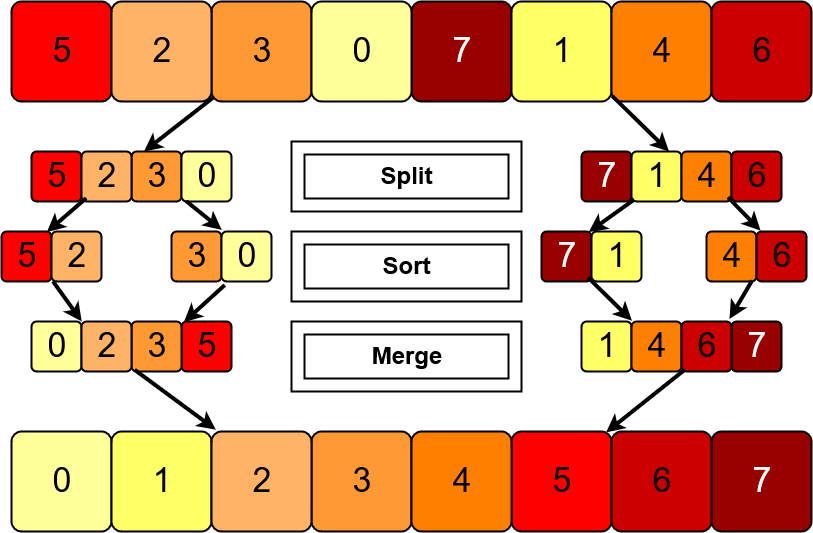
\includegraphics[width=0.45\textwidth]{merge_sort.png}
\caption{Parallel merge-sort algorithm scheme.
Starting from the original array the master thread split the work (sub-arrays) along two slaves threads (\textsf{split} step in the graph).
The split recursion is applied until a required size of sub-arrays is reached.
Each slave-thread applied a sort function (\textsf{sort} step in the graph).
Then the full array is recombined following back the thread recursion applying an \textsf{inplace-merge} function (\textsf{merge} step in the graph).
}
\label{fig:merge_sort}
\end{figure}

As parallelization strategy we can yet invoke the new \emph{keywords} of OpenMP libraries and apply a \emph{divide-and-conquer} architecture using a tree of independent \emph{tasks}\footnote{
  Tasks in OpenMP are code blocks that the compiler wraps up and makes available to be executed in parallel.
}.
Using the maximum power of two of the available threads we split the computation in equal size sub-arrays and perform independent \textsf{argsort}s.
Then, going backwards to the subdivisions at each step we merge the sub-arrays two-by-two until the root.


\end{document}
 % parallel merge-sort
\documentclass{standalone}


\begin{document}

\subsection[Network Signature]{Network signature}\label{implementation:network}

After the rearrangement of feature pairs in ascending order we can start to create the variable network and looking for its connected components as putative signatures.
Each feature will be represent a node in the network and a given pair will be a connection between them.
Since the full storage of the network would require a matrix $(N\times N)$, we have to chose a better strategy for the processing\footnote{
  We are working in the hypothesis of very large $N$.
}.

The ordered set of couples computed in the previous section represents a so-called \emph{COO sparse matrix} (Coordinate Format sparse matrix) and we can reasonable assume that the desired signature will be composed by the top ranking of them.
So, the first step will be to cut a reasonable percentage of the full set of pairs and process only them.

Moreover, we are interested in a small set of variables unknown a prior.
The load of all the node pairs into the same graph can slow down the computation.
An iterative method (with stop criteria) can perform better in the large case of samples and only in worst cases the full set of pair will be loaded.

Since the described algorithm step does not require particular performance efficiency now, the main code used in our simulation was written in pure \textsf{Python}.
A \textsf{C++} implementation of the same algorithm was developed with the help of the Boost Graph Library~\cite{BGL} (BGL), but to not overweight the code installation, it was reserved just for a style exercise.
In this section we discuss about this second version and also about the strategies chosen to implement an efficiency version of it.
This version of the algorithm was also used as stand alone method for other applications that will be presented later.

BGL is a very wide framework for graph analysis based on template structures.
The library efficiency discourage the users to re-implement the same algorithms and, for the current purposes, it was resulted more than sufficient.

Starting from the top scorer feature pairs, we progressively add each couple of nodes to an empty graph.
At each iteration step, the number of connected components is evaluated until a desired number of nodes (greater or equal) is not reached\footnote{
  This procedure is quite similar to put a threshold value on the couple performances or just simpler highlight inside the full network the components linked by weights greater than a given value.
}.
Two degree of freedom are left to the user: in order, \textsf{pruning} and \textsf{merging}.
The first one performs an iteratively remotion of nodes with degree equal (or lower) than 1, i.e pendant nodes, until the graph core is not filtered.
The \textsf{merging} clause choose between the biggest connected component or the the set of all the disjoint connect components as putative signature.
The output of \textsf{merging} step determine the number of nodes in the graph which have been considered for the stop criteria.

A crucial role in the optimization of the algorithm is played by the chosen BGL graph structure.
Since the two degree of freedom imply a continuous rearrangement of the graph nodes, the strategy chosen is to apply a filter mask over the main graph structure that highlights the only part of interest.
This can be done using the \textsf{boost :: filtered\_graph} object of BGL.
In ~\ref{code:featuresel} the \textsf{C++} snippet is shown.

\lstset{style=c++}
\begin{lstlisting}[language=C++, caption=DNetPRO signature extraction, label=code:featuresel]
#include <boost/graph/adjacency_list.hpp>
#include <boost/graph/connected_components.hpp>
#include <boost/graph/filtered_graph.hpp>
#include <boost/function.hpp>
#include <boost/graph/iteration_macros.hpp>

typedef typename boost :: adjacency_list< boost :: vecS, boost :: vecS, boost :: undirectedS, boost :: property< boost :: vertex_color_t, int >, boost :: property < boost :: edge_index_t, int > > Graph;
using V = Graph :: vertex_descriptor;
using Filtered = boost :: filtered_graph < Graph, boost :: keep_all, boost :: function < bool(V) > >;


std :: vector < int > FeatureSelection (int ** couples, const int & min_size, bool pruning=true,  bool merging=true)
{
  Graph G;
  std :: set < V > removed_set;
  Filtered Signature (G, boost :: keep_all {}, [] (V v) {return removed_set.end() == removed_set.find(v);});

  int L = 0, leave, Ncomp, i = 0;

  while ( true ){

    boost :: add_edge (couples[i][0], couples[i][1], G);

    while ( pruning ){

      leave = 0;
      BGL_FORALL_VERTICES (v, Signature, Filtered);
        if ( boost :: in_degree (v, Signature) < 2 ){
          removed_set.insert (v);
          ++ leave;
        }

      if ( leave == 0 )
        break;
    }

    if ( num_vertices (G) - removed_set.size() ){

      components.resize (num_vertices (G));

      Ncomp = boost :: connected_components (Signature, &components[0]);

      if ( merging ){

        BGL_FORALL_VERTICES (v, Signature, Filtered)
          if ( boost :: in_degree(v, Signature) )
            core.push_back ( static_cast < int >(v) );
      }
      else {

        std :: map < int, int > size;
        for ( auto && comp : components ) ++ size[comp];

        auto max_key = std :: max_element (std :: begin(size), std :: end(size),
                                           [] (const decltype(size) :: value_type && p1, const decltype(size) :: value_type && p2)
                                           { return p1.second < p2.second; })->first;

        BGL_FORALL_VERTICES (v, Signature, Filtered)
          if ( components[v] == max_key )
            core.push_back( static_cast < int >(v) );
      }

      components.resize (0);
      L = static_cast < int >(core.size());
    }

    removed_set.clear();

    if ( L >= min_size ) break;

    ++ i;

    core.resize (0);
  }

  return core;
}

\end{lstlisting}

In the above description, it should be clear that, given any set of ordered (in ascending order) couples of variables, this algorithm allows to extract the core network independently by the procedure which generate them.
So it can be used as dimensionality reduction algorithm of general purpose network structures.
An example of this kind of application was reported in Appendix B - Venice Road Network in which we summarized the results of~\cite{Mizzi2018, CurtiSDPS2018}.

\end{document}

 % feat sel algorithm
\documentclass{standalone}


\begin{document}


\subsection[Python wrap]{DNetPRO in Python}\label{implementation:python}

Up to now we are focusing on the algorithm performances leaving out the usability of the DNetPRO algorithm for the (research) community.
Despite the C++ is one of the most efficient and old programming language\footnote{
  Still in common use in scientific research groups.
}, the Python language users are increasing in the last few years.
Python is becoming leader in scientific research publications and the large part of Machine Learning analysis are performed using Python libraries (in particular \emph{scikit-learn} library).
So we have to reach a compromise between the performances and usability of new developed codes and it can be reached using the Cython~\cite{behnel2010cython} framework.

Cython \quotes{language}\footnote{
  It is not a real programming language since it is based on Python.
  However it has its own syntax and keywords which are different either from Python either from C++.
  In the end it needs a compiler to run and it is certainly different from Python.
} allows an easy interface between C++ codes and Python language.
With a relatively simple wrapping of the C++ functions they can be used inside a pure Python code preserving as much as possible the computational performances of the pure C++ version.
In this way we can create a simple Python object which performs the full set of DNetPRO steps and moreover which is compatible with the functions provided by the other machine learning libraries.

With this purposes we chose to operate a double wrap of the C++ functions to separate as much as possible the C++ component from the Python one\footnote{
  Cython wrap are very powerful tools for C++ integration into Python code but, by experience, they are difficult to manage by pure-Python users.
  A simple workaround is to perform a first wrap of the C++ function inside a Cython object and a second wrap of it into a pure-Python one.
  This two-steps wrap certainly gets worse the computational performances but it allows a complete separation between the compiled part of the code (Cython) and the interpreted (Python) one.
  Moreover we can leave back all the checks on input parameters
  in the C++ version since they will be performed at run time in the Python wrap.
}.
The Python object was written considering a full compatibility with the \emph{scikit-learn} library to allow the use of the DNetPRO feature selection as an alternative component of other Machine Learning pipelines.


\end{document}
 % python wrap with sklearn compatibility
\documentclass{standalone}


\begin{document}

\subsection[Pipeline]{DNetPRO in Snakemake}\label{implementation:snakemake}

The starting (silent) hypothesis done until now is that we are running the DNetPRO algorithm on a single dataset (or better on a single Hold-Out subdivision of our data).
On this configuration it is legal to stress as much as possible the available computational resources and parallel processing each step of the algorithm.

If we want to introduce our algorithm inside a larger pipeline, in which we compare the resulting obtained over a Cross-Validation of our datasets we have to re-think about the parallelization done.
In this case, each fold of the cross validation can be interpreted as an independent task and, following the main programming rule \emph{\quotes{parallelize the outer, vectorize the inner}}, we should spawn a thread for each fold and perform the couple evaluation in sequential mode.
Certainly, the optimal solution would be to separate our jobs across a wide range of inter-connected computers and still perform the same computation in parallel but it would required to implement our hybrid (\textsf{C++} and \textsf{Python}) pipeline in a Message Passing Interface (MPI) environment.

An easier solution to overcome all these problems can raise by the use of \textsf{SnakeMake}~\cite{snakemake} rules.
\textsf{SnakeMake} is an intermediate language between \textsf{Python} and \textsf{Make}.
Its syntax is almost like the \textsf{Make} language, but with the help of the easier and powerful \textsf{Python} functions.
It is widely used for bioinformatic pipeline parallelization since it can easily applied over single or multi-cluster environment (master-slave scheme) with a simple change of command line.

\begin{center}
\begin{figure}[htbp]
\hspace{-2cm}
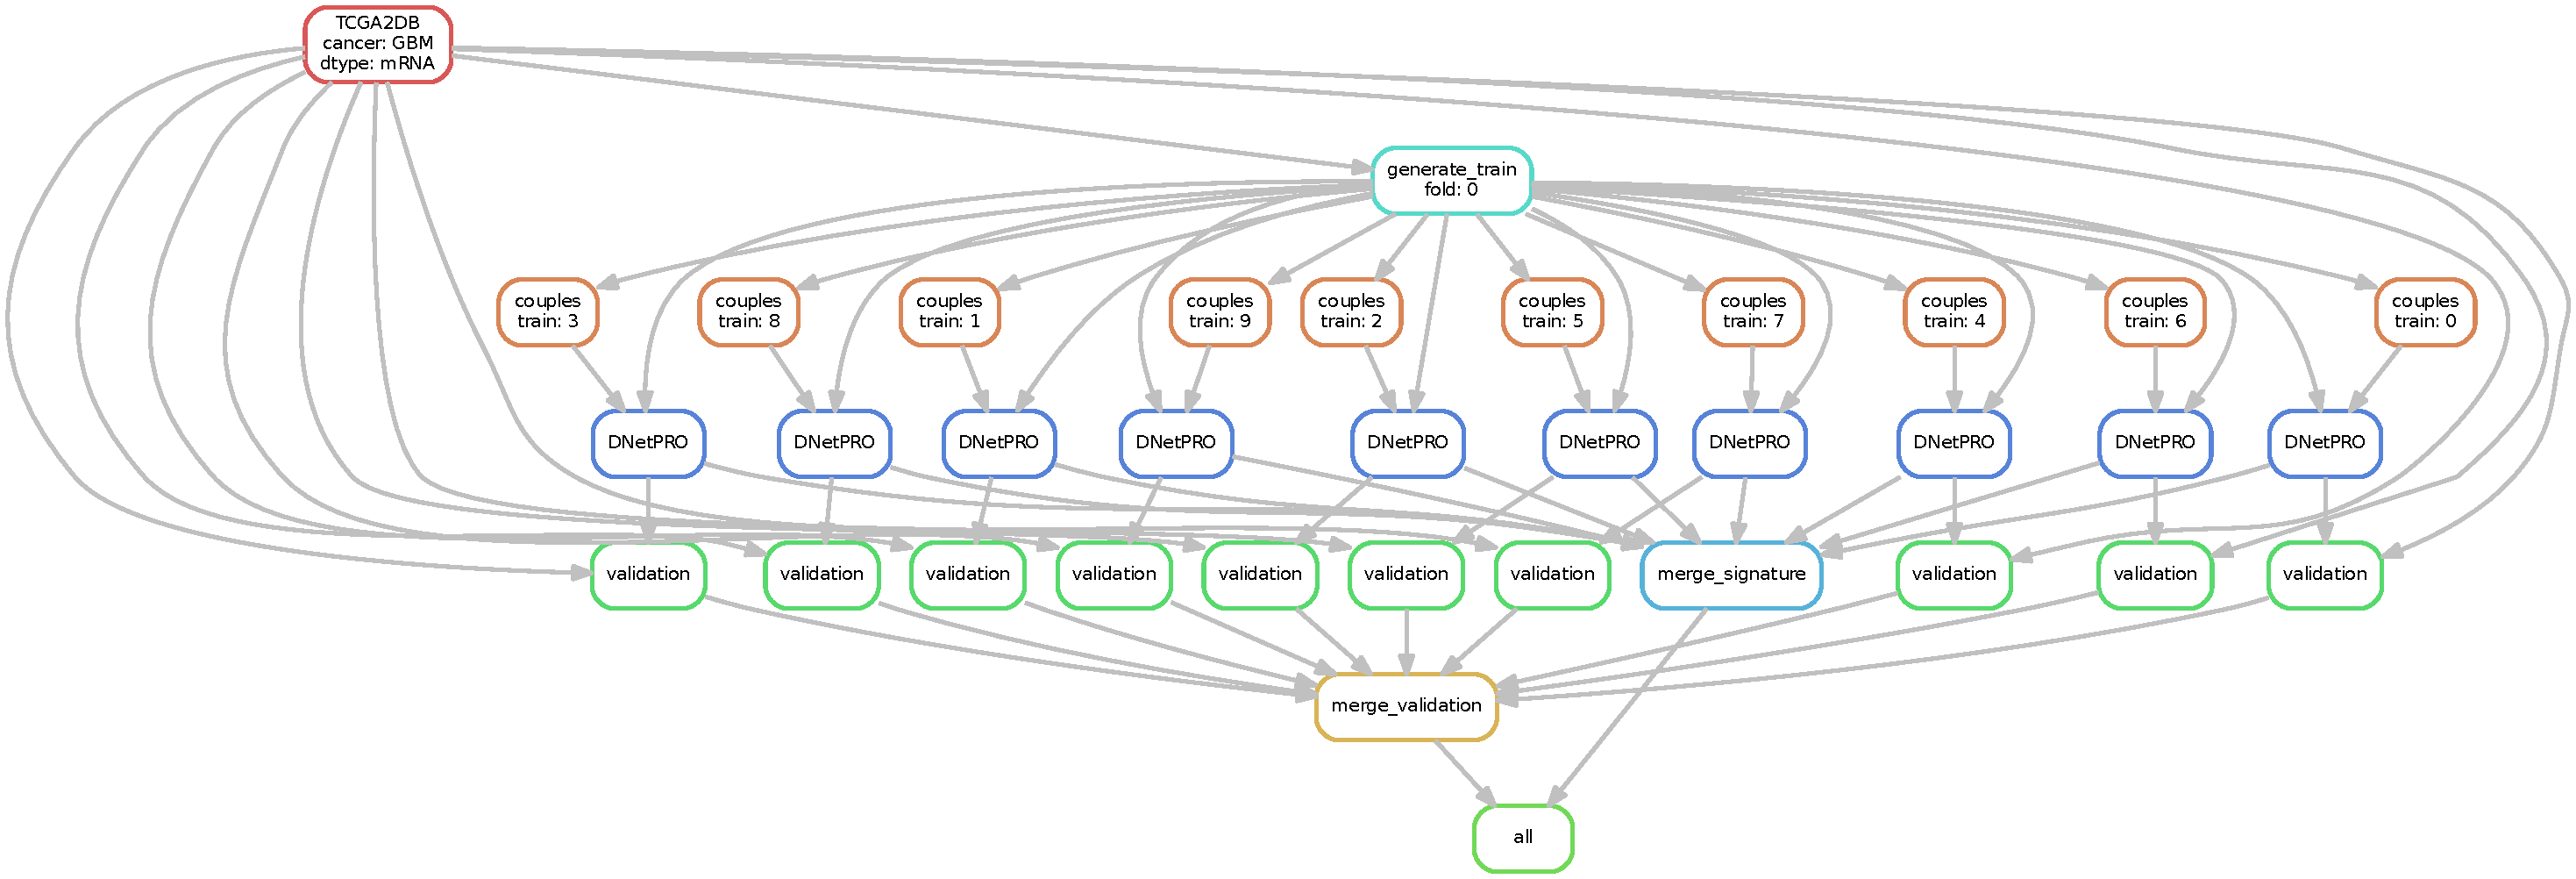
\includegraphics[width=1.3\textwidth]{qdanet_pipe_single.pdf}
\caption{Example of DNetPRO pipeline on a single cross validation.
It is highlighted the independence of each fold from each other.
This scheme shows a possible distribution of the jobs on a multi-threading architecture or for a distributed computing architecture.
The second case allows further parallelization scheme (hidden in the graph) for each internal step (e.g. the evaluation of each pair of genes).
}
\label{fig:dnet_workflow}
\end{figure}
\end{center}

So to improve the scalability of our algorithm we implement the benchmark pipeline scheme using Snakemake rules and a work-flow example for a single cross-validation is shown in Fig.~\ref{fig:dnet_workflow}.
In this case each step of Fig.~\ref{fig:dnet_workflow} can be performed by a different computer unit preserving the multi-threading steps, with a maximum scalability and the possibility to enlarge the problem size and the number of variables.


\end{document}
 % pipeline description with snakemake
\documentclass{standalone}


\begin{document}

\subsection[Time performances]{Time performances}\label{implementation:timing}

As described in the above sections the DNetPRO is a combinatorial algorithm and thus it requires a particular accuracy in the code implementation to optimize as much as possible the computational performances.
The theoretical optimization strategies described until now have to be proofed by quantitative measures.

We tested the computational performances of our Cython (C++ wrap) implementation against the pure Python (naive) implementation shown in \ref{code:py_couples}.
The time evaluation was performed using the \textsf{timing} Python package in which we can easily simulate multiple run of a given algorithm\footnote{
  We would stress that we can use the \textsf{timing} Python package only because we provided a Cython wrap of our DNetPRO algorithm implementation.
  We would also highlight that, albeit minimal, the Python superstructure penalizes the computational performances and the best results can be obtained using the pure C++ version of the code.
}.
In our simulations we monitored the three main parameters related to the algorithm efficiency: the number of samples, the number of variables and (as we provided a parallel multi threading implementation) the number of threads used.
For each combination of parameters we performed 30 runs of both algorithms and we extracted the minimum execution time.
The tests were performed on a classical bioinformatics server (128~GB RAM memory and 2 CPU E5-2620, with 8 cores each)
The obtained results are shown in Fig.~\ref{fig:dnetpro_timing}.
In each plot we fixed two variables and we evaluated the remaining one.

\begin{figure}[htbp]
\def\svgwidth{0.4\textwidth}
\input{./img/features_timing.pdf_tex}
\qquad\qquad
\centering
\def\svgwidth{0.4\textwidth}
\input{./img/samples_timing.pdf_tex}
\qquad\qquad
\centering
\def\svgwidth{0.5\textwidth}
\input{./img/nth_timing.pdf_tex}
\caption{Execution time of DNetPRO algorithm.
We compare the execution time between pure-Python and Cython (C++ wrap) implementation.
\textbf{(a - left)} Execution time in function of the number of variables (the number of samples and the number of threads are kept fixed).
\textbf{(b - right)} Execution time in function of the number of samples (the number of variables and the number of threads are kept fixed).
\textbf{(c - bottom)} Execution time in function of the number of threads (the number of variables and the number of samples are kept fixed).
}
\label{fig:dnetpro_timing}
\end{figure}

In all our simulations the efficiency of the (optimized) Cython version is easily visible and the gap between the two implementations reached more than $10^4$ seconds.
On the other hand is important to highlight the scalability of the codes against the various parameters.
While the code performances scales quite well with the number of features (Fig.~\ref{fig:dnetpro_timing}(a)) in both the implementations, we have a different trend varying the number of samples (Fig.~\ref{fig:dnetpro_timing}(b)): the Cython trend starts to saturate almost immediately while the computational time of the Python implementation continues to grow.
This behavior highlights the results of the optimizations performed on the Cython implementation which allows the application of the DNetPRO algorithm also to larger datasets without loosing performances.
An opposite behavior is found monitoring the number of threads (ref Fig.~\ref{fig:dnetpro_timing}(c)): the Python version scales quite well with the number of threads\footnote{
  The optimal result should be a linear scalability with the number of threads but it is always difficult to reach this efficiency.
  Thus, a reasonable good result is given by a progressive decrease with increasing the number of threads.
}, while Cython trend is more unstable.
This behavior is probably due to a not optimized schedule in the parallel section: the work is not equally distributed along the available threads and it penalizes the code efficiency creating a bottleneck related to the slowest thread.
The above results are computed considering a number of features equal to 90 and thus the parallel section distributes the 180 ($N\times N$) iterations along the available threads: when the number of iterations is proportional to the number of threads used (12, 20 and 30 in our case) we have a maximization of the time performances.
Despite this, the computational efficiency of the Cython implementation is so better than the Python one that its usage is indisputable.

\end{document}
 % timing performances

\documentclass{standalone}

\begin{document}

\section[Benchmark]{Benchmark of DNetPRO algorithm}\label{synapse:benchmark}

Up to now we have been talked about the DNetPRO algorithm from a theoretical point-of-view.
Starting from this section we discuss about the application of the algorithm on real biological datasets (see Appendix B - Venice Road Network for results obtained on a different kind of data).

Despite previous version of the DNetPRO method were already applied on biological data~\cite{PMrna, Scotlandi2009, PMgene, Terragna} a wide range benchmark of it was still missing.
In the following sections we describe the results obtained on the Synapse dataset and published in~\cite{Curti2019}.

\end{document}
 % Introduction ot TCGA dataset
\documentclass{standalone}

\begin{document}

\subsection[Synapse]{Synapse dataset}\label{synapse:synapse}

As benchmark dataset was chosen the core sets extracted from the The Cancer Genome Atlas (accession number \href{https://www.synapse.org/#!Synapse:syn300013/wiki/27406}{syn300013, doi:10.7303/syn300013}) (\emph{Synapse dataset} in the following), used in a previous study~\cite{Yuan2014} which aimed at quantifying the role of different omics data types (e.g. mRNA and miRNA microarray data,  protein levels measured with Reverse Phase Protein Array - RPPA) via different state-of-the-art classification methods.
This allowed us to compare our results to a large set of commonly used classification methods, by using their performance validation pipeline (accession number \href{https://www.synapse.org/#!Synapse:syn1710282/wiki/27303}{syn1710282, doi:10.7303/syn1710282}).

The Synapse dataset is composed by four tumors datasets: kidney renal clear cell carcinoma (KIRC), glioblastoma multiforme (GBM), ovarian serous cystadenocarcinoma (OV) and lung squamous cell carcinoma (LUSC).
For each cancer type we applied the \textsf{DNetPRO} algorithm on mRNA, miRNA and RPPA data and we compare the performances results with the Yuan et al. ones.

The summary description of the datasets used is reported in the Tab.~\ref{tab:synapse}.

\begin{table}[htbp]
\centering
\begin{tabular}{lccccccc}
\hline \rowcolor{darkgrayrow}
         &               &                &          & Number       \\
\rowcolor{darkgrayrow}
Cancer   & mRNA          & miRNA          & Protein  & of samples   \\
\hline
GBM      & AgilentG4502A & H-miRNA\_8x15k & RPPA     &              \\
         & 17814         & 533            & $^a$     & 210          \\
KIRC     & HiseV2        & GA+Hiseq       & RPPA                    \\
         & 20530         & 1045           & 166      & 243          \\
OV       & AgilentG4502A & H-miRNA\_8x15k & RPPA     &              \\
         & 17814         & 798            & 165      & 379          \\
LUSC     & HiseqV2       & GA+Hiseq       & RPPA     &              \\
         & 20530         & 1045           & 174      & 121          \\
\hline
\end{tabular}
\caption{In the first row platforms are reported and the second shows the dimension of dataset as number of probes.
AgilentG4502A: Agilent 244K Custom Gene Expression G4502A;
HiseqV2: Illumina HiSeq 2000 RNA Sequencing V2;
H-miRNA\_8x15K: Agilent 8~×~15K Human miRNA-specific microarray platform;
GA+Hiseq: Illumina Genome Analyzer/HiSeq 2000 miRNA sequencing platform;
RPPA: MD Anderson reverse phase protein array.
The last column shows the number of sample.
\newline $^a$ Missing data-type for that cancer type.
}
\label{tab:synapse}
\end{table}

Each tumor dataset was pre-processed by adding a zero-mean Gaussian random noise ($\sigma = 10^{-4}$)) to remove the possible null values in the database, which could produce numerical errors in the distances evaluation between genes.
Then, we randomly split each dataset in training and test sets with a stratified (i.e. balanced for class sample ratio) 10-fold procedure: with the stratification we are reasonably sure that each training-set is a good representative of the whole sample set.
The choice of a 10-fold splitting is aimed to reproduce the analysis pipeline presented by Yuan et al. with an analogous cross-validation procedure.
Since we don't have exact details of their data splitting, the cross validation was repeated 100 times, for a total of 1000 training procedures for each tumor (OV, LUSC, KIRC, GB) and data type (mRNA, miRNA, RPPA).
Each training procedure led to the extraction of multiple signatures.

We chose threshold values in order to obtain a resulting number of variables (network nodes) in the order of $10^2-10^3$, and identified all connected components of the network as signatures.
If more than one component existed, each one was considered as a different signature.

The final multidimensional signatures were tested by a Discriminant Analysis with a diag-quadratic distance, to avoid possible problems about covariance matrix inversion (as for the Mahalanobis distance).

\begin{center}
\begin{figure}[htbp]
\centering
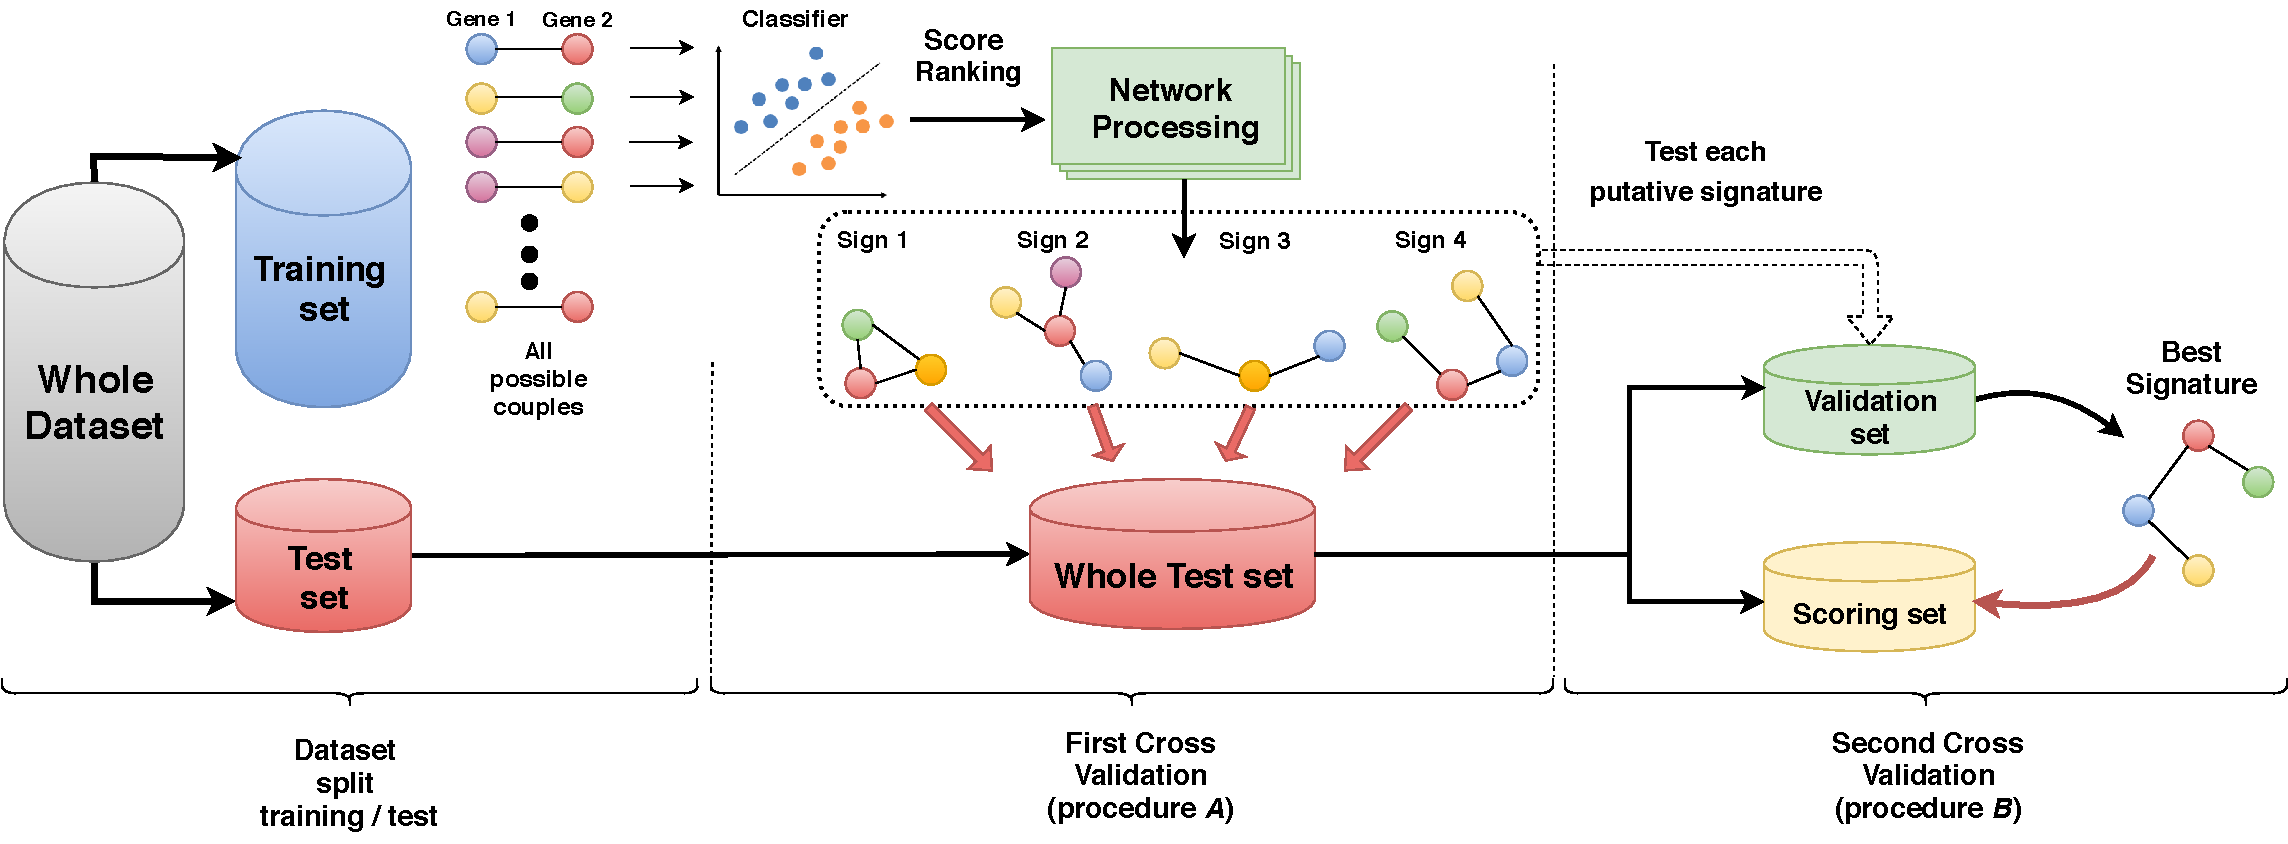
\includegraphics[width=1.0\textwidth]{dnet_pipe.pdf}
\caption{Scheme of \textsf{DNetPRO} algorithm.
On the \quotes{training set}, all possible couples of variables are used for Discriminant Analysis, generating the fully connected network weighted by classification performance.
Thresholding ranked couples, several signatures can result (as connected components) and their performance is evaluated on the \quotes{whole test set} (procedure $A$).
% Signatures are given by the connected components created by all couples with scorer greater than a chosen threshold.
A unique best signature can be identified on a \quotes{validation set} and tested in a \quotes{scoring set}, obtained by further splitting the \quotes{whole test set} (procedure $B$).
% The pipeline parameters was adapted to faithfully mimic the reference work-flow to allow a comparison of the final results except for the second cross validation step.
}
\label{fig:dnet_pipe}
\end{figure}
\end{center}

We remark that \textsf{DNetPRO} can provide more than one signature as a final outcome, given by all the connected components found in the variable network, or a unique top-performing signature can be obtained by a further cross-validation step (procedure $A$ and procedure $B$ in Fig.~\ref{fig:dnet_pipe}, respectively).

In the single cross validation configuration (procedure $A$ in Fig.~\ref{fig:dnet_pipe}), the best signature was extracted as the one reaching the highest accuracy score during the training step.
This best signature was then tested over the available test set.

When also the second cross validation was used (procedure $B$ in Fig.~\ref{fig:dnet_pipe}) the best signature wasted as the most performing over a subset of the whole test set (\emph{validation set}), and the final performance was evaluated on the remaining \emph{scoring set}.

To compare our results with the work of Yuan et al., we used the AUC (\emph{Area Under the Curve}) score, that they provided in the paper as the result of their analyses.
The distribution of our results could be compared to the single score value given in the other work.

\end{document}
 % dataset description
\documentclass{standalone}

\begin{document}

\subsection[mRNA data]{mRNA dataset}\label{synapse:mRNA}

We applied both training procedure (ref.~\ref{fig:dnet_pipe}) on the mRNA dataset.
The results are shown, as distribution of AUC (Area under the curve) score, in Fig.~\ref{fig:dnet_results}~(a) for the best signatures obtained with procedure $A$ (corresponding to the validation approach used in~\cite{Yuan2014}), while results with the full cross-validation procedure $B$ are shown in Fig.~\ref{fig:dnet_results}~(b).

As expected, performances decrease with the introduction of the second cross validation step, but the values remain quite stable showing the robustness of the extracted signatures, and we remark that the validation procedure used in the reference paper by Yuan et al. resembles our approach without the second validation step.

\begin{figure}[htbp]
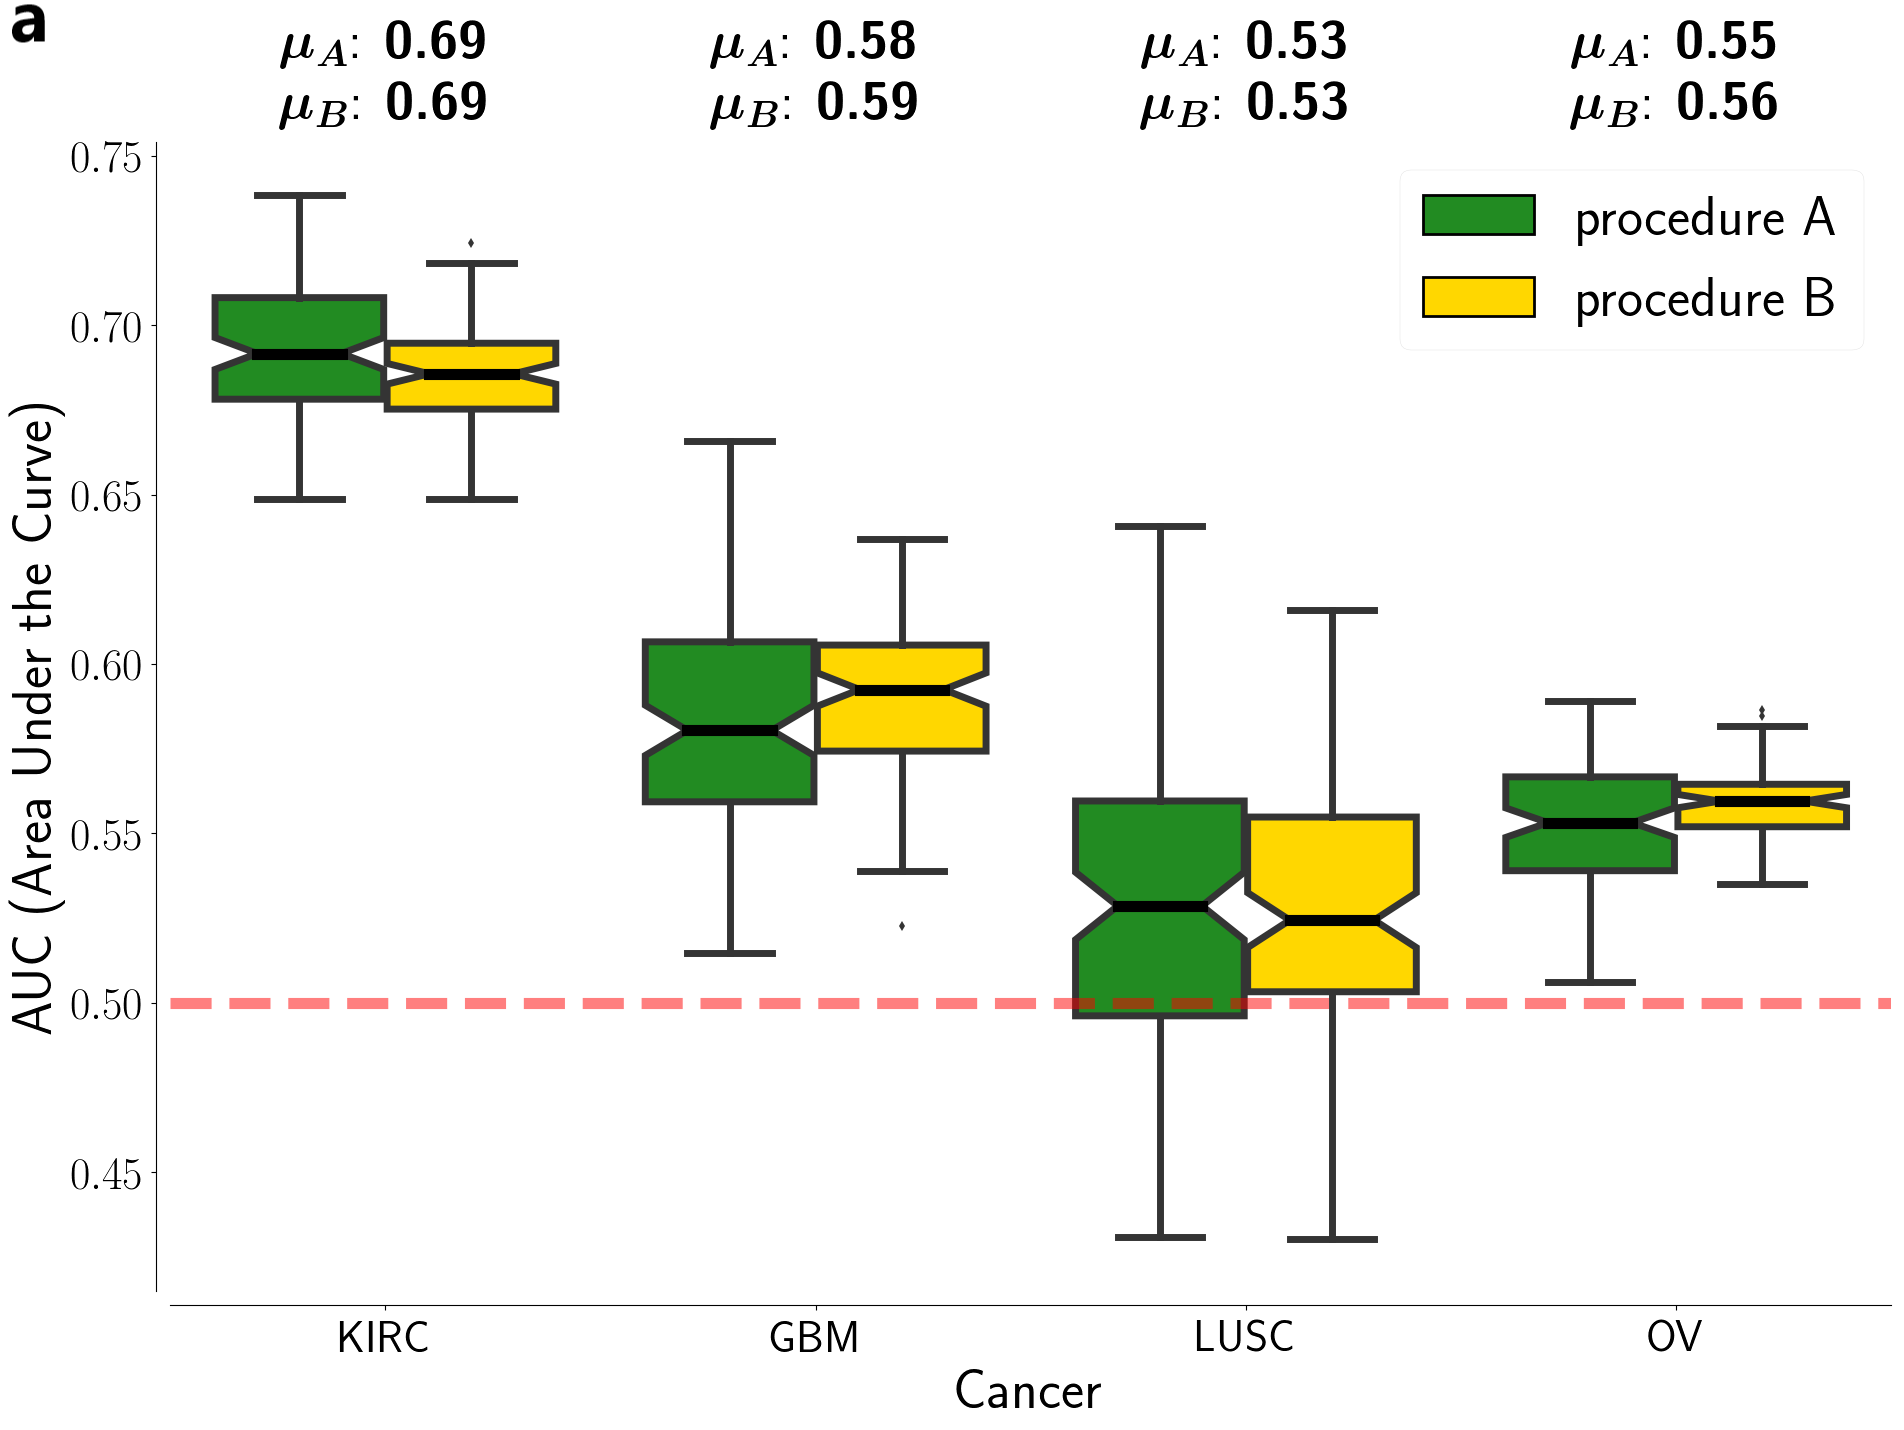
\includegraphics[width=0.4\textwidth]{mRNA_boxplot.png}
\qquad\qquad
\centering
\def\svgwidth{0.45\textwidth}
\input{./img/mRNA_tables.pdf_tex}
\caption{Results obtained by the DNetPRO algorithm pipeline on four mRNA tumor datasets, as from the Synapse database~\cite{Yuan2014}.
\textbf{(a)} Distributions of AUC values for the tumor datasets. Green boxplots: results using procedure $A$ as described in Fig.~\ref{fig:dnet_pipe}; yellow boxplots: results obtained using procedure $B$.
\textbf{(b)} Comparison of DNetPRO results with the methods used in the paper of Yuan et al.: max AUC values obtained over the 10-Fold cross-validation procedure.
}
\label{fig:dnet_results}
\end{figure}

All results are comparable (LUSC) or better (KIRC, GBM) than the results reported in~\cite{Yuan2014}, except for the OV dataset, also with the more conservative approach involving a further cross-validation step.
The size of the extracted signatures is quite constant, and smaller than 500 genes in each pipeline execution.
Analogous results are obtained also for the miRNA dataset, in which our method outperforms in three over four cases, while the RPPA dataset shows less significant results (Supplementary material).

To test the robustness of our method, since each cross-validation procedure may generate different signatures, we measured the overlap of the genes belonging to each mRNA signature over 100 simulations with different training-test data splitting.
We observed an average overlap ranging from 40\% to 60\%, with a smaller group of genes found across all the 100 cross-validation iterations.

In this application the DNetPRO algorithm has several advantages: easy scalability on parallel architectures, simple signature interpretation allowing a valuable application in a biomedical context and a significant robustness in a highly noisy environment such as genomics measurements.

\end{document}
 % mRNA results
\documentclass{standalone}

\begin{document}

\subsection[miRNA and RPPA data]{miRNA and RPPA dataset}\label{miRNA}

\end{document}
 % miRNA and RPPA results
\documentclass{standalone}

\begin{document}

\subsection[Ranking]{Couple ranking}\label{synapse:ranking}

Since the number of variable pairs is typically very large (e.g. $10^8$ pairs with gene expression microarrays containing about $10^4$ probes) many of them may achieve the same performance, since the possible performance values are integer number typically in a limited range (corresponding to the number of available samples, $10^2-10^3$ in many cases).
Therefore, the ranking of pairs by their performance is characterized by multiple \quotes{plateaus}(Fig.~\ref{fig:plateaus}(a)), and the selection of probe pairs based on a hard thresholding procedure is highly influenced by this feature.
Monitoring this trend behavior can be noticed that only a few number of pairs belongs to the first performances chunks and while the performances decrease multiple pairs and features appear, as it can be seen in Fig.~\ref{fig:plateaus}(a).

This kind of trend highlight the difficulty on finding informative features inside the huge noise of other variables and it gives us a constrain in the developing of a realistic biological toy model.
Moreover it confirms us that a putative signature could be made by only a few amount of central genes at least weakly connected with other noise nodes.

\begin{figure}[htbp]
\centering
\def\svgwidth{0.4\textwidth}
\input{./img/lengths.pdf_tex}
\qquad\qquad
\def\svgwidth{0.4\textwidth}
\input{./img/plateaus.pdf_tex}
\caption{Analysis of ranked pairs distributions according to the performance score obtained in the training step.
(\textbf{a}) The distribution of plateau lengths is approximately exponential.
(\textbf{b}) Average number of pairs with the same score value: this behavior is typical in ranking order distribution and it can be fitted by the relation $f(x) = A(M + 1 - r)^b / r^a$ as shown in~\cite{rankfit}, where $r$ is the rank value, $M$ its maximum value, $A$ a normalization constant and ($a$, $b$) two fitting exponents.}
\label{fig:plateaus}
\end{figure}

As in other cases of ranked values~\cite{rankfit}, we can fit these ranking distributions with a combination of power-law functions obtaining a good agreement with experimental points (Fig.~\ref{fig:plateaus}(b)).

We also observed that \emph{star}-networks frequently appear, with one variable highly connected to many others which are only connected with it.
This happens when a variable has a strong discriminating power, to which other possibly less relevant variables get linked for noisy fluctuations.

As stated before, we suggest that these variables (pendant nodes in the star network) can be removed from the signature without significantly affecting its performance.
The procedure can be applied for one single step (in order to remove nodes pending from a star configuration) or it can be applied recursively, until the signature becomes constituted only by the 2-core network (i.e. with all nodes having degree $\geq2$).
Empirical analysis performed on real data has shown that the removal of these variables does not affect significantly the signature performance, and in the meanwhile it allows a significant reduction of its dimensionality.
Since there is no clear theoretical explanation of this behavior, we suggest to introduce this step only optionally, since it is not easy to quantify the risk of loosing relevant information from the removed variables.

The underlying idea is that the more connected are the nodes, the more the variables in the signature \quotes{work well} together, a plausible hypothesis given the linear sample separation surface provided by the Discriminant classifier.
Moreover, the network structure of the signature suggests further considerations about the relevance of a variable as a function of its role in the network (e.g. node centrality such as degree or betweenness centrality).

\end{document}
 % ranking couples conclusions
\documentclass{standalone}

\begin{document}

\subsection[Signature Overlap]{Characterization of signature overlap}\label{synapse:overlap}

In the analysis of the Synapse dataset we used a complex pipeline of cross-validation (ref Fig.~\ref{fig:dnet_pipe}) to obtain a sufficient statistics.
The DNetPRO algorithm was designed to work on a single dataset since the signature extraction can involve different variables for different data subdivisions.
In our application we divide the dataset into a training-test subdivision and the signature were extracted along a 10-fold cross-validation over the training set.
This kind of setup could produce 10 totally different signatures, in the worst case.
Moreover we replicated our simulation for 100 repetitions and thus a set of 1000 totally independent signatures were extracted.

Starting from this large subset of variables we can evaluate the robustness of the DNetPRO algorithm in the variable identifications studying the overlap between these signatures.
From a statistical point-of-view is quite unlikely that the same set of variables were included into all the extracted signatures, especially on this application, in which the variable roles are assumed by genes.
On the other hand the overlap of these signatures could highlight a statistical significance of some variables and thus genes related to the understudied tumors.

As case study we analyzed only the KIRC mRNA dataset in which the extracted signatures ranged from 4 to 650 genes ($\mu=382$ genes).
For each gene we counted its occurrences along the 1000 signatures.
The same analysis was performed taking into account the signatures generated using the $K$-best score variables (ref.~\ref{dnetpro:toy} for further informations) and a random features extraction.
In Fig.~\ref{fig:overlap} the genes distribution obtained by the three methods are shown.

\begin{figure}[htbp]
\centering
\def\svgwidth{0.6\textwidth}
\input{./img/DNetPRO_overlap.pdf_tex}
\caption{Signatures overlap obtained in the KIRC mRNA datasets.
Genes occurrences of the 1000 DNetPRO signatures extracted from the Synapse pipeline (blue).
Genes occurrences of the 1000 $K$-best variables extracted from the Synapse pipeline (red): the number of genes ($K$) is the same of the corresponding DNetPRO signature.
Genes occurrences of 1000 random signatures (yellow).
}
\label{fig:overlap}
\end{figure}

Both DNetPRO and $K$-best feature extraction algorithms identified a core set of genes common to the full set of signatures.
The $K$-best algorithm appears more stable than the DNetPRO algorithm and it is easier to find the same genes along the extracted signatures.
This behavior could be associated to the problems highlight also in the toy model simulations (ref. \ref{dnetpro:toy}): the DNetPRO algorithm is able to identify only one signature but the informative features (genes) could not co-operate in the same network-signature and thus they could be discarded.
The DNetPRO signatures are, in fact, very small compared to the number of variables and thus only small network components were extracted which are very closed to star-networks.
Despite the discrepancy between the signatures we have a core of 18 genes which occurs in at least the 95\% of both signatures and 8 of them are in the 99\% of both signatures.

The common genes were also mapped on public databases (TISIDB~\cite{10.1093/bioinformatics/btz210} and Oncotarget~\cite{
%TODO:MISS REF (search KIRC LTB4R on google)
}, which link tumors to related genes.
We found 14/18 genes as informative probes for the KIRC tumor in the TISIDB and 7 of them were also found in the Oncotarget database\footnote{
  The list of genes in the TISIDB cover \quotes{only} 988 genes.
  From our list we have only one gene which was found in the Oncotarget database and not in the TISIDB.
  This gene misses in the TISIDB so we can not evaluate its importance.
}.
Taking into account the core set of 8 genes we found 3 of them on Oncotarget database and 7 of them on the TISIDB.
The only exception was given by the LOC388796 gene which was not found in any database.

The random feature extraction method is not even comparable with the others and it simply represents a null model.

\end{document}
 % overlap of signatures

\documentclass{standalone}

\begin{document}

\section[Cytokinoma Dataset]{Cytokinoma dataset}\label{cytokine}

Increasing evidence suggests that inflammation is involved in Alzheimer's disease (AD) pathogenesis.
Elevated peripheral levels of different cytokines and chemokines in subjects affected by AD compared with healthy control (CTL) have emphasized the role of peripheral inflammation in the disease.
Thus, these proteins can represent specific factors of disease development and progression.
Considering the cross-talking between the central nervous system and the periphery, the inflammatory analytes may provide utility as biomarkers to identify AD at earlier stages, in particular for the diagnosis of Mild Cognitive Impairment (MCI), a condition at risk of development of dementia.
AD is a major neurocognitive disorder and the most common cause of dementia in the old age, accounting for 60\% to 80\% of all causes.
During the past decade, a conceptual shift occurred in the field of AD considering the disease as a continuum.
In this context, there is an urgent need for biomarkers identification able to accurately detect AD in an early stage, before the appearance of neurologic signs.
An early diagnosis can hopefully lead to a better and more effective treatment, which could potentially limit neuronal damage and prevent the development of overt AD.
An emerging field in the study of neuroinflammation is the sex-related differences: in the last years, gender studies have been increasingly developed with the aim to adopt gender differences as a key to interpretation many diseases, including neurodegenerative diseases.

Experimental data showed that many mechanisms are involved in AD pathogenesis including neuroinflammation.
The dysregulation of cytokines and chemokines is a central feature in the development of neuroinflammation, neurodegeneration, and demyelination both in the central and peripheral nervous systems.
Among many chemokines and cytokines, pro-inflammatory IFN$\alpha$2, TNF$\alpha$, and IL-1$\alpha$ are described as heterogeneously implicated in AD pathogenesis.

The interactive network of cytokines/chemokines, defined as \quotes{cytokinome}, is extremely complex.
Using the DNetPRO algorithm as statistical feature selection method, we might discriminate the groups and propose a useful tool to follow the progression and evolution of AD from its early stages, also in light of gender differences.
With this study, we aimed first at the identification of a potential proteins profile able to discriminate AD, MCI and CTL and, therefore identify a potential early and easy to get a diagnostic marker of subjects at risk.

\end{document}
 % Introduction to Cytokine
\documentclass{standalone}

\begin{document}

\subsection[Dataset]{Dataset}\label{cytokine:cytokine_data}

In this case-control observational study, we evaluated $289$ old-age subjects referred to our Geriatric Memory Clinic.
The dataset comprises $189$ female and $100$ male individuals with a mean age of $78.6$ ($\pm7.5$) years.
The date were provided by the co-authors of this project at the Institute of Gerontology and Geriatrics at the University of Perugia (Department of Medicine).
For each patient a set of 26 cytokine expression level were computed with the additional information about subject sex, age and diagnosis label (AD, MCI or CTL).
Of the 289 enrolled subjects, the whole set of cytokines was available for 284 subjects (98\%), specifically 87/88 CTL (99\%), 70/73 MCI (96\%), 127/129 AD (98\%).

To approximate normal distribution, plasma cytokines and chemokines were log-transformed for data analyses.
For the analysis of single cytokines with respect to the CTL, MCI and AD group, we designed a linear model analysis, with the value of each cytokine as a linear combination of the subject group (with CTL samples as the baseline, and MCI, AD as conditions), age and sex, as factors (the formula representation would be \quotes{cytokine $\sim$ group + sex + age}).
The last two were included as possible confounding factors, even if the analyses revealed that their role for each cytokine is marginal.
Only IFN$\alpha$2, IL-1$\alpha$, and MCP-1 differed among groups after correction for age and sex.
A threshold $p<0.05$ was considered for significance at all levels (group, sex or age).

Then we applied the \textsf{DNetPRO} algorithm looking for a signature capable of discriminating between CTL and AD: to this purpose, we performed a Hold-Out cross-validation procedure to identify the cytokine signature, considering 2/3 of samples to train the model and then we tested the signature performance on the remaining 1/3 of the total samples.
In this analysis we did not separate male from female samples, to avoid the bias given by the uneven number of samples in these two groups, and since previous analysis at a single-cytokine level did not find significant differences due to sex.
Then, we classified MCI samples with the CTL-AD signature obtained in the previous step, that allowed labeling MCI samples as CTL or non-CTL.

%Description of the cytokinoma dataset with statistics.
%Application of the \textsf{DNetPRO} on the Cytokine dataset.
%Discussion on the obtained signature and biological %interpretation of the Alzheimer disease.


\end{document} % Dataset description
\documentclass{standalone}

\begin{document}

\subsection[Results]{Resuls}\label{cytokine:cytokine_result}

The best signature identified to discriminate between CTL and AD subjects is composed of three cytokines, IFN$\alpha$2, TNF$\alpha$, and IL-1$\alpha$.
Its total accuracy on the CTL-AD test set is 65.27\% (with 61\% CTL and 66\% AD correctly classified).
The sensitivity/specificity values for classification is reported in Tab.~\ref{tab:cytokine}.

\begin{table}[!htb]
  \begin{minipage}{.5\linewidth}
    \hspace{-1.5cm}
      \begin{tabular}{cccc}
          \hline \rowcolor{darkgrayrow}
                      &  \textbf{Accuracy}  &  \textbf{Sensitivity}  &  \textbf{Specificity} \\
                      &  AD vs. CTL         &  AD                    &    CTL                \\
          \hline
              Men     &    16/25            &    8/12                &    8/13               \\
                      &          (64.00\%)  &         (66.67\%)      &         (61.54\%)     \\
              Women   &    33/48            &   27/38                &    6/10               \\
                      &          (68.75\%)  &         (71.05\%)      &         (60.00\%)     \\
              Total   &    47/72            &   36/54                &   11/18               \\
                      &          (65.24\%)  &         (66.66\%)      &         (61.11\%)     \\
          \hline
      \end{tabular}
  \end{minipage}%
  \begin{minipage}{.5\linewidth}
    \hspace{.5cm}
      \begin{tabular}{ccc}
          \hline \rowcolor{darkgrayrow}
                        \textbf{Prediction} &  \textbf{Sensitivity}  &  \textbf{Specificity} \\
                         MCI as non-CTL     &  MCI                   &    CTL                \\
          \hline
                           15/26            &   15/26                &   24/36               \\
                                 (57.69\%)  &         (57.69\%)      &         (66.67\%)     \\
                           41/47            &   41/47                &   23/51               \\
                                 (87.23\%)  &         (87.23\%)      &         (45.09\%)     \\
                           62/73            &   62/73                &   36/87               \\
                                 (84.93\%)  &         (84.93\%)      &         (41.38\%)     \\
          \hline
      \end{tabular}
  \end{minipage}
  \caption{The sensitivity/specificity values for AD vs CTL classification by the 3-protein signature, for the total sample dataset and stratified by sex.
    The second table shows the result of predictions of MCI samples with the same signature as non-CTL samples.
    In this case the sensitivity and specificity were computed in relation to the CTL in the training set.
  }
  \label{tab:cytokine}
\end{table}


\begin{figure}[htbp]
\hspace{-1.0cm}
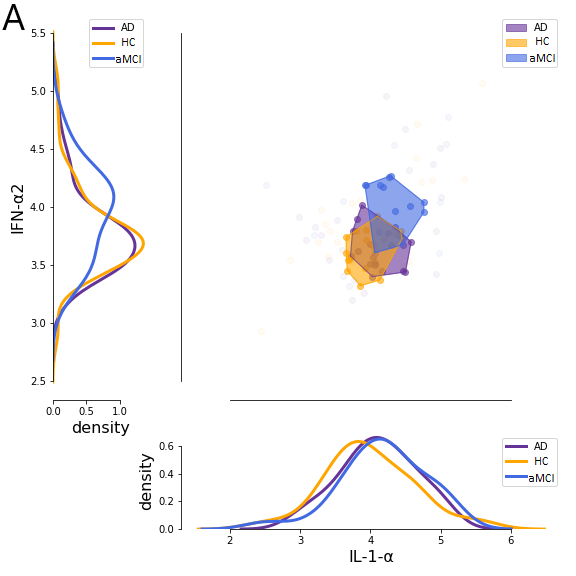
\includegraphics[width=0.45\textwidth]{males.png}
\qquad\qquad
\hspace{1.0cm}
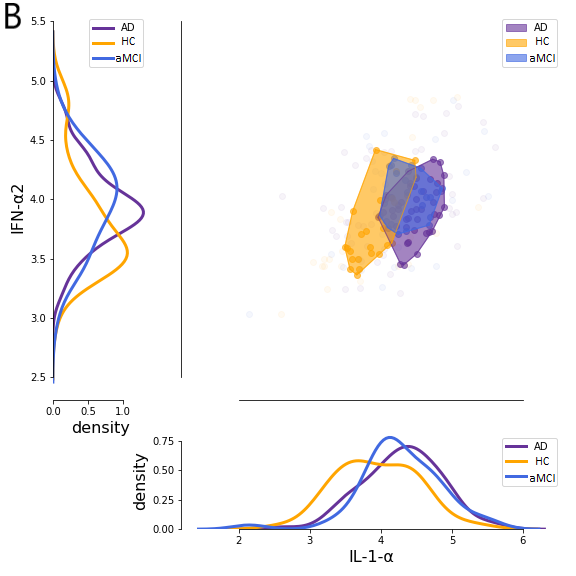
\includegraphics[width=0.45\textwidth]{females.png}
\caption{\textbf{(A)} Scatter plot of IL-1$\alpha$ and IFN-$\alpha$, and distribution plot for the single cytokines along the axes, stratified by diagnostic group (AD, CTL, and MCI) in \textbf{males}.
In this case, the HC group is less separated from aMCI and AD.
\textbf{(B)} Scatter plot of IL-1$\alpha$ and IFN-$\alpha$, and distribution plot for the single cytokines along the axes, stratified by diagnostic group (AD, CTL, and MCI) in \textbf{females}.
In this case, the HC group is well separated from aMCI and AD.
}
\label{fig:cytokine_sex}
\end{figure}

Applying this signature to classify MCI vs CTL samples, it correctly predicted 84.93\% of MCI as \quotes{non-CTL}.
Two cytokines from the signature, IFN$\alpha$2 and IL-1$\alpha$, showed a significant difference between groups also at a single cytokine level in previous analyses.
We plotted them as a representative in all population and stratified the scatter plots by sex (ref Fig.~\ref{fig:cytokine_sex} A, B).
The CTL group resulted better separated from MCI and AD in women as compared with men.
The trajectory of the subject groups moves from CLT to AD, and interestingly the identified signature is able to differentiate MCI from CLT better than from AD.
This is a promising result since it seems more useful to recognize MCI from CLT than full-blown AD from CLT.
Probably the poor sensibility in detecting AD could be linked to the disease evolution that makes nebulous and vague the cytokine pattern in the brain of these patients, as confirmed from several studies that found both up-regulation and down-regulation of many cytokines in AD cerebral samples.
This fact could be more accentuated in our population of old age subjects in which markers of aging are often mixed with those of dementia.

In this study we show that: 1) an easy to get cytokines signature composed of three molecules - IFN$\alpha$2, TNF$\alpha$, and IL-1$\alpha$ - is able to discriminate the studied groups;  2) the combination of IFN$\alpha$2 and IL-1$\alpha$ able to distinguish CTL from  MCI and AD better in women than in men.
Sex (referred to biological differences) and gender (psychosocial and cultural differences) affect human brain biology throughout individual lifespans, affecting male and female cognitive functions differently.
Epidemiological studies show that women have a higher risk of AD as well as a higher dementia prevalence, particularly in the old age, as compared with men.

In conclusion, the identified cytokinome signature shows a good accuracy in differentiating aMCI from CTL, especially in female.
Understanding sex differences will help to define individualized preventive and treatment interventions for AD.

\end{document} % result

\documentclass{standalone}

\begin{document}

\section[Bovine Dataset]{Bovine Paratuberculosis}\label{bovine:bovine}

Paratuberculosis or Johne's disease (JD) in cattle is a chronic granulomatous gastroenteritis caused by infection with \emph{Mycobacterium avium subspecies paratuberculosis} (MAP).
JD is not treatable; therefore the early identification and isolation of infected animals is a key point to reduce its incidence worldwide.
In this work DNetPRO algorithm was applied to RNAseq experimental data of 5 cattle positive to MAP infection compared to 5 negative uninfected controls.
The purpose was to find a small set of differentially expressed genes able to discriminate between infected animals in a pre-clinical phase.
Results of the DNetPRO algorithm identified a small set of 10 transcripts that differentiate between potentially infected, but clinically healthy, animals belonging to paratuberculosis positive herds and negative unexposed animals.
Furthermore, the same set of 10 transcripts differentiate negative unexposed animals from positive animals based on the results of the ELISA test\footnote{
  The enzyme-linked immunosorbent assay.
  It is a common diagnostic tool as well as a quality control check in various bio-medical industries and in medicine.
} for bovine paratuberculosis and fecal culture.
Within the 10 transcripts that together had good discriminative potential, 5 (TRPV4, RIC8B, IL5RA, ERF and CDC40) show significant differential expression between the three groups while the remaining 5 transcripts (RDM1, EPHX1, STAU1, TLE1, ASB8) did not show a significant differences in at least one of the pairwise comparisons.
In conclusion, the discriminant analysis described here identified a set of 10 genes that discriminate between the exposed and sero-converted animals.
When tested in a larger cohort, these finding lead the possible use of RNA expression analysis as new diagnostic test for paratuberculosis.
Such a signature could allow early interventions to reduce the sanitary and economic burden, and to reduce the risk of infection spreading.

In the next sections a description of the dataset and of main DNetPRO results will be discussed.
Further informations can found in the original paper~\cite{Malvisi2019}.

\end{document}
 % Introduction to Bovine
\documentclass{standalone}

\begin{document}

\subsection[Dataset]{Dataset}\label{bovine_data}

Paratuberculosis or Johne's disease (JD) in cattle is a chronic granulomatous gastroenteritis caused by infection with \emph{Mycobacterium avium subspecies paratuberculosis} (MAP).
JD is present worldwide, is a welfare issue and causes significant economic losses.
Cattle are usually infected as young calves but typically do not show clinical signs before 24 months of age, however not all infected animals progress to clinical disease.
JD is not treatable, therefore the early identification and isolation of infected animals, before they start shedding the bacteria, is a key point to reduce its incidence in cattle herds worldwide.
In addition, an association between MAP and Crohn's disease (CD) in humans has been suggested and intensively explored.
Given the economic losses and welfare concerns for livestock, and possible human health risk, the research interest in JD has been driven by the substantial difficulty in early diagnosis of infected animals and the exploration of potentially new diagnostic techniques.

The dataset used in this work was previously discussed and generated by some of the authors of the original paper.
In detail, the dataset used comprised 15036 transcripts from 15 samples, classified as \quotes{serologically negative non exposed cows/healthy} (5 samples, labeled as NN), \quotes{serologically negative exposed cows/ infected} (5 samples, NP) and \quotes{serologically positive cows/clinical} (5 samples, PP).
Only transcripts with non-zero measures for all samples were considered, reducing the dataset to 13529 transcripts.

All data generated or analyzed during this study is available upon request, furthermore all transcript counts per sample are given as supplementary information files of the original paper.


\end{document}
 % Dataset description
\documentclass{standalone}

\begin{document}

\subsection[Results]{Bovine Signature}\label{bovine:bovine_result}

In the context of high-throughput data analysis, a challenge is the search for an optimal choice of variables (a \quotes{signature}) to classify groups of samples or regress trends with optimal performance and minimum dimensionality.
Usually high-throughput omics data (e.g. transcriptomics, ge-nomics, methylomics) provide datasets with few tens to hundreds of samples, and often 1000 times larger numbers of variables.
The objective of dimensionality reduction through the choice of an optimal signature is twofold: 1) the identification of relevant variables, that should separate the signal from the noise (i.e. variables not significantly associated to, or descriptive of the studied process); 2) in a practical context, it is important to establish future diagnostic criteria that can be implemented in cheap and simple toolkits, such as PCR cards or dedicated microarray chips, that usually test a small number of transcripts (ranging from tens to hundreds, at most).
The quantity of samples compared to the available features of this work, join with the final purposes of this kind of analysis, set the well-known ill-posed problem conditions for which the DNetPRO algorithm was thought.

Since the number of sample is drastically small no robust cross-validation procedure can be applied.
So we focused on the identification of a putative gene-signature able to discriminate between NN and NP samples, leaving the PP data as validation set.
In this case we hypothesize that PP samples will be classified more closely with NP sample rather than NN as exposed, possibly infected samples, should be more similar to positive samples, than to negative controls.

\begin{figure}[htbp]
\centering
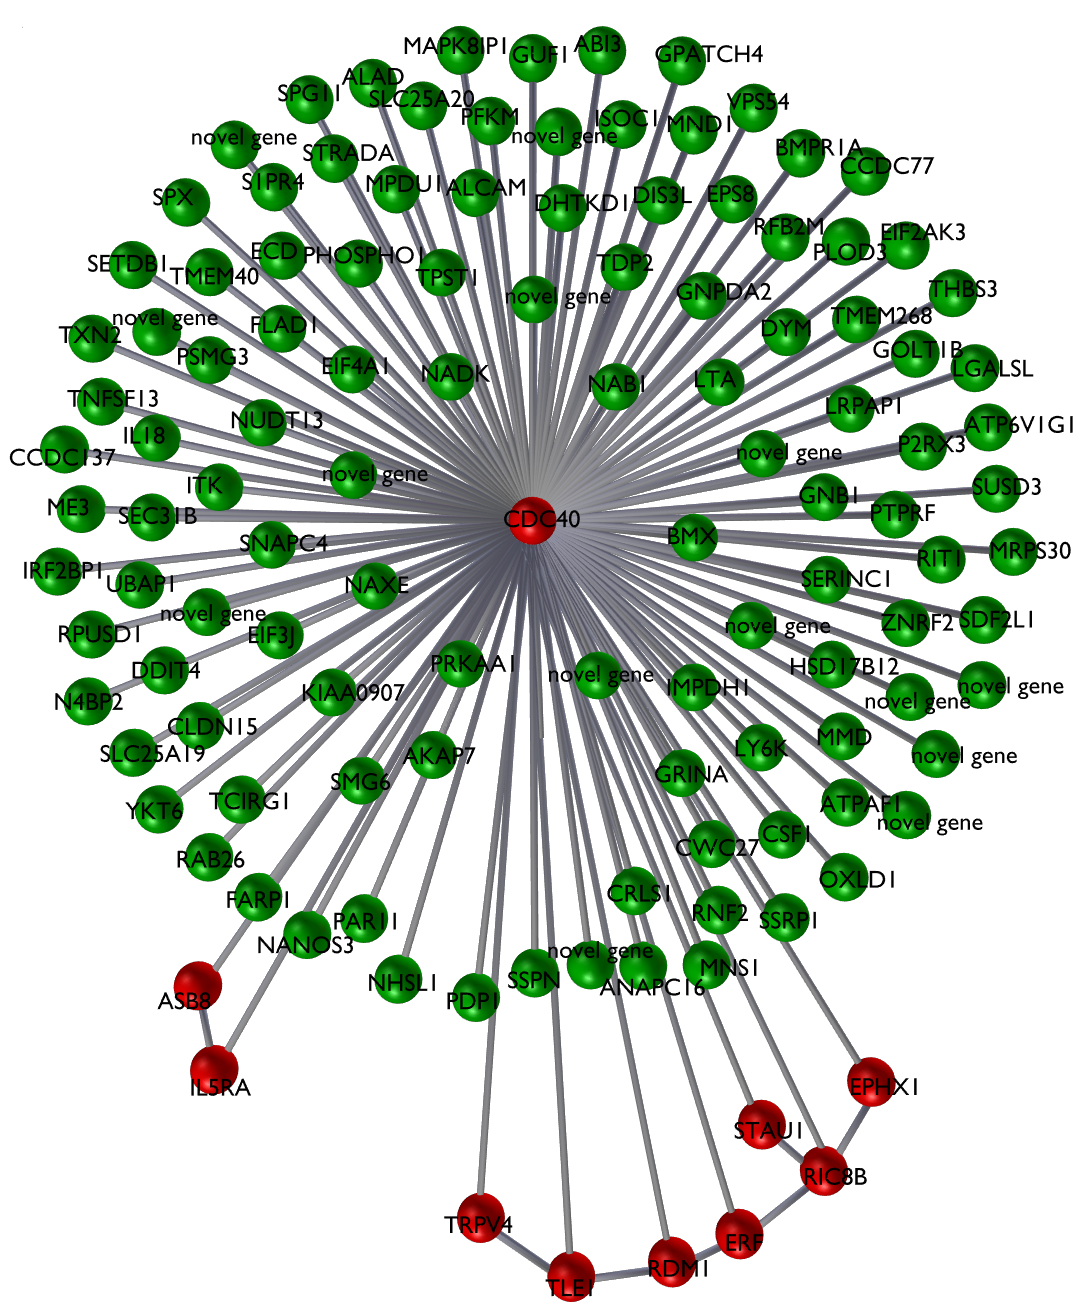
\includegraphics[width=0.4\textwidth]{Bovine_signature.png}
\qquad\qquad
\def\svgwidth{0.45\textwidth}
\input{./img/Bovine_expression_level.pdf_tex}
\caption[Caption Bovine]{(\textbf{a}) Plot of the 123-transcript network, with a details of the 10-probe signature (red nodes)\footnotemark.
(\textbf{b}) Transcript levels for the 10 genes belonging to the classification signature identified by the combinatorial discriminant analysis (CDA).
Some transcripts (EPHX1, RIC8B, IL5RA, ERF, CDC40) show a clear trend  between 5 animals serologically positive to the ELISA test for MAP (PP), 5 exposed serologically negative (NP) and 5 serologically negative unexposed control animals (NN).
}
\label{fig:bovine_signature}
\end{figure}
\footnotetext{
  The figure was generated using a custom network visualizer described in Appendix C - BlendNet.
}


Starting from the top-performing couples of transcripts, we obtained an initial signature of 123 different transcripts (Fig~\ref{fig:bovine_signature}(a), all the nodes), capable to correctly classify 4 out of the 5 NN samples (80\%) and all 5 NP samples (100\% performance).
The average performance was therefore 90\% with Matthews correlation coefficient MCC = 0.82.
Processing the 123-transcript network by removing all pendant nodes (i.e. removing all single transcripts belonging to only one best-performing couple) we obtained a final signature with 10 transcripts with a 100\% performance classifying all NN and NP samples (Fig~\ref{fig:bovine_signature}(a), only red nodes).
As it can be seen, many nodes are directly connected to the central node (belonging to the 10-transcript signature), while only the 10 transcripts of the signature are also connected between each other.

Principal Component Analysis of the 10-transcript signature showed that in many cases there was a progressive increase or decrease in the transcript levels when passing from a healthy (NN) sample to a positive (PP) sample, passing through the infected (NP) sample class.
Fig~\ref{fig:bovine_signature}(b) shows the expression levels of the transcripts belonging to the signature for all samples.

To further validate the goodness of the signature, we generated 10000 different signatures with 10 randomly chosen transcripts, and then applied a Leave-One-Out cross validation procedure to classify all 15 samples with these signatures.
Comparing the performance of the random signatures with the true 10-transcript signature, only 50 of these signatures (corresponding to 0.5\% of the random signature distribution) produced better performance than our signature in terms of classification performance, confirming its high significance.

We even characterized the possible biological role of the signature genes, among the significantly differentially expressed genes, the cell division cycle 40 gene (CDC40) showed the smallest fold change between classes.
However in the identified signature the CDC40 gene is the most central node associated with the health status of the animals related to JD.
CDC40 was also under expressed in the NP and PP groups, compared with the NN group and it has been shown to be involved in clathrin medated endcytosis from a biological point-of-view.
Clathrin is the best characterized coat protein involved in the endocytosis process, specifically in receptor-mediated-internalization.
\emph{Mycobacterium paratuberculosis} enters the host macrophages, its primary target cell, and manages to survive within their phagosome.
It is possible that the under-expression of CDC40 in infected and sick animals compared to unexposed animals may be associate with down regulation of macrophage genes post mycobacterial invasion, facilitating the survival of the pathogen with the host target cell.

Interestingly within the set of 10 discriminating transcripts, in addition to CDC40, others show links with immune response mechanisms, these include IL5RA, ERF and TRPV4.
These genes potentially have functions related to the biology of progression of JD.
Also for the other genes of the final 10-transcript signature a possible biological interpretation related to JD was given (see the original paper for further descriptions).

In conclusion, the DNetPRO algorithm identified a set of 10 genes, the expression levels of which could discriminate between the exposed and sero-converted animals.
These finding lead the possible use of RNA expression analysis as new diagnostic test for JD.
In particular the approach may be able to identify infected animals prior to sero-conversion, prior to a positive ELISA test result.
However, further tests for specificity and validation in a larger cohort are required.


%Description of the bovine dataset with biological background.
%Application of the DNetPRO on the Bovine dataset with the description of the two singatures extracted.
%Discussion on biological interpretation of the genes.

% cite and describe BlendNet repo in the signature figure

\end{document}
 % results and conclusion

\end{document}

% Introduction to feature selection problem and theoretical background. Focus on biological Big Data and problems related.
% Description of the method and efficiency a biological toy model.
% Description of the algorithm implementation with focus on performances of the new implementation.
% Application of the DNetPRO on the Synapse dataset (mRNA, miRNA, RPPA) of Yuan et al. with discussion about obtained performances compared with the most common ML methods and signature characterization
% Application of the DNetPRO on the Cytokine dataset with data description and obtained results
% Application of the DNetPRO on the Bovini dataset with data description and obtained results with biological interpretation


%% Chapter 2 - Neural Network and Byron

\documentclass{standalone}

\begin{document}


\documentclass{standalone}

\begin{document}

\chapter[Deep Learning]{Deep Learning - Neural Network algorithms}\label{chapter2:neural}

In the first chapter we have discussed about the difficulties on extracting information from a huge amount of data, and we have proposed a novel feature selection algorithm to face these problems.
Those kind of applications go under the wide research field of Machine Learning.
Machine learning algorithms are closely related to a statistical interpretation of the available data.
With the increasing availability of computational power and data it is not always possible to tune and build an accurate model able to describe the heterogeneity of our samples.
Many everyday problems involve very complex tasks, and we are interested on models able to solve many tasks at the same time.
From a machine learning point-of-view this can be achieved building pipelines, i.e work-flows made by multiple steps of processing, which aim to simulate as much close as possible the human intelligence.
This leads us into the Deep Learning research field, in which very computational expensive models have been built to face general purpose problems, often related to real time applications.

The description of a deep learning model is quite often given by a Neural Network architecture, i.e a more or less complex pipeline of functions which takes in input a sample and it applies a series of transformations and filters to obtain the required result.
All these pipelines are very computational expensive and they require appropriate optimization strategies.

In this chapter we introduce some of the most common functions related to deep learning applications, giving a very fast mathematical explanation of them and carefully focusing on their numerical issues and solutions.
We start from an introduction about general Neural Network models up to some of modern deep learning models, involving object detection, image segmentation and image super resolution.
In particular, we describe two custom libraries (\textsf{NumPyNet} and \textsf{Byron}) developed by the author of this thesis, for educational and analytical purposes, respectively.
Both libraries are released with MIT license and the codes are publicly available on my Github page (\href{https://github.com/Nico-Curti/Byron}{Byron} and \href{https://github.com/Nico-Curti/NumPyNet}{NumPyNet}).
These libraries have already used in several applications and in the last sections we show some of the obtained results\footnote{
  Both \textsf{NumPyNet} and \textsf{Byron} libraries have been developed with the collaboration of master degree students and several thesis have their applications as core arguments.
}.

In the last section of this chapter we introduce a different kind of Neural Network model, the \textsf{Replicated Focusing Belief Propagation} (rFBP) model.
This model has solid physical and statistical bases and we discuss about its novel optimized implementation, available on my Github (\href{https://github.com/Nico-Curti/rFBP}{Replicated Focusing Belief Propagation}) and released under MIT license.
This model differs from standard deep learning neural networks changing the updating rule and we show its first application on real data.

\end{document}
 % Neural Network introduction

\documentclass{standalone}

\begin{document}

\section[Neural Network models]{Neural Network models}\label{nn}

Neural Networks are mathematical models commonly used in data analysis.
They are becoming a standard tool in Machine Learning and Deep Learning research and many complex problems can be easily solved by these models.
From a theoretical point-of-view we can define a Neural Network as a series of non-linear multi-parametric functions.
The model parameters are tuned during a so called \emph{training section} in which we feed our model with a set of data with human supervision, i.e we have prior knowledge about the right and desired output of the model.
After the training section we can verify the efficiency of our training using a new set of data, called \emph{test set}, which is never seen by the model.
If we have prior knowledge about the output of our test set we can compute the accuracy (or more generally the score) of our model; in the other case we will simply have an extrapolation of our data.

A wide range of documentations and implementations have been written on this topic and it is more and more hard to move around the different sources.
Leader on this topic are became the multiple open-source Python libraries available on-line as \emph{Tensorflow}~\cite{tensorflow2015-whitepaper}, \emph{Pytorch}~\cite{paszke2017automatic} and \emph{Caffè}~\cite{Jia:2014:Caffe}.
Their portability and efficiency are closely related on the simplicity of the Python language and on the simplicity in writing complex models in a minimum number of code lines.
Only a small part of the research community uses more deeper implementation in C++ or other low-level programming languages.
About them it should be mentioned the \emph{darknet project} which created a sort of standard in object detection applications using a pure Ansi-C library.

In this section we firstly retrace the mathematical background of these models.
To each theoretical explanation we discuss the numerical problems associated and we provide an efficient custom implementation of each algorithm.
The numerical aspects will be traced following two  developed custom libraries: NumPyNet library~\cite{NumPyNet} and Byron library~\cite{Byron}.

NumPyNet was born as educational framework for the study of Neural Network models.
It is written trying to balance code readability and computational performances and it is enriched with a large documentation to better understand the functionality of each script.
The library is written in pure Python and the only external library used is Numpy~\cite{Numpy} (a based package for the scientific research).

Despite all common libraries are correlated by a wide documentation is often difficult for novel users to move around the many hyper-links and papers cite in it.
NumPyNet tries to overcome this problem with a minimal mathematical documentation associated to each script and a wide range of comments inside the code.

An other \quotes{problem} to take in count is related to performances.
Libraries like \emph{Tensorflow} as certainly efficient by a computational point-of-view and the numerous wrappers (like \emph{Keras} library) guarantees an extremely simple user interface.
On the other hand the deeper functionality of the code and the implementation strategies used are unavoidably hidden behind tons of code lines.
In this way the user can performs complex computational tasks using the library as black-box package.
NumPyNet wants to overcome this problem using simple Python codes with extremely readability also for novel users to better understand the symmetry between mathematical formulas and code.

The simplicity of this library we will allow to give a first numerical analysis of the model functions and, moreover, to show the results of each function to a simple image to better understand the effects of their applications on real data\footnote{
  Aware of the author no other example implementations have been done.
  This makes the NumPyNet library a useful tool for neural network study and a virtual laboratory for new neural network functions.
}.
Each NumPyNet function was tested against the \emph{Tensorflow} implementation of the same methods with an automatic testing routine through \emph{PyTest}~\cite{Okken:2017:PTP:3176124}.
The full code is open-source on the Github page of the project.
Its installation is guaranteed by a continuous integration framework of the code through \emph{Travis CI} for Unix environments and \emph{Appevyor CI} for Windows users.
The library supports Python version $\ge2.6$\footnote{
  The library provides also an \textsf{Image} object to load and process images.
  The object is based on OpenCV API~\cite{OpenCV}.
  OpenCV does not yet support Python version 2.7 and 3.3 so the whole NumPyNet package does not work on these two version of Python.
  You can just exclude the \textsf{Image} scripts from the package or use a novel wrap based on different library (e.g \textsf{Pillow}).
}.

As term of comparison we will discuss the more sophisticated implementations into the Byron library.
Byron (Build YouR Own Neural network) library is written in pure C++ with the support of the modern standard 17.
We deeply use the c++17 functionality to reach the better performances and flexibility of our code.
What makes Byron an efficient alternative to the competition is the complete multi-threading environment in which it works.
Despite the most common Neural Network libraries are optimized for GPU environments, there are only few code implementations which exploit the fully functionality of a multiple CPUs architecture.
This gap discourage multiple research groups on the use of such computational intensive models in their applications.
Byron works in a fully parallel section in which is single computational function is performed using the full set of available cores.
To further reduce the time of thread spawn and so optimize as much as possible the code performances, the library works using a single parallel section which is opened at the beginning of the computation and closed at the end\footnote{
  For real-time applications also the time required for the thread spawn must be taken into account.
}.

The Byron library is release under MIT license and public available on the Github page of the project.
The project also includes a list of common examples like object detection, super resolution, segmentation, ecc. (see the next sections for further details about this models).
The library is also completely wrapped using \emph{Cython} to enlarge the range of users also to the Python ones.
The complete guide to its installation is provided; it can be done using \emph{CMake}, \emph{Make} or \emph{Docker} and the Python version is available with a simple \emph{setup}.
The testing of each function is performed using \emph{Pytest} automatic framework against the NumPyNet implementation (faster and lighter to import than \emph{Tensorflow}).

We will use Byron library as term of comparison with the other common library used in Neural Network models and for each function we test its computational efficiency and scalability on multiple cores.
Two machines will be used in the computational testing: a common laptop (8~GB RAM memory and 1 CPU i7-6500U, with 2 cores) and a classical bioinformatics server (128~GB RAM memory and 2 CPU E5-2620, with 8 cores each).

Starting from the next section we introduce the fundamental Neural Network model, the so-called \emph{Simple Perceptron}.
From the simplest model we will add complexity layers to overcome the relative problems (mathematical and numerical), introducing the main functionality of the modern Neural Network architectures.

\end{document}

\documentclass{standalone}

\begin{document}

\subsection[Simple Perceptron]{Simple Perceptron}\label{NN:perceptron}

The fundamental unit of each Neural Network model is the \emph{simple Perceptron} (or single neuron).
The \emph{Perceptron} it the simpler mathematical model of biological neuron and it is based on the Rosenblatt~\cite{Rosenblatt58theperceptron} model which identifies a neuron as a computational unit with input, synaptic weights and an activation threshold (or function).
Following the biological model of Hodgkin and Huxley~\cite{HHmodel} (H-H model), we have an action potential, i.e the output of the neuron, given by

$$
y = \sigma\left(\sum_{i=1}^{N}w_i x_i + w_0 \right)
$$
\\
where $\sigma$ is the activation function, $w_i$ are the synaptic weights and $x_i$ the inputs.
The $w_0$ coefficient identifies the bias of the linear combination and it is left as parameter to be tune by the optimization algorithm (learning phase).

The connection weights $w_i$ are tuned during the training section by the chosen updating rule.
The standard updating rule is simply given by

$$
w_i(\tau + 1) = w_i(\tau) + \gamma(t - y)x
$$
\\
where $\gamma$ is the gain or step size ($\gamma \in [0, 1]$) and $t$ is the desired output.
In other words we have to firstly compute the difference between the current output and the desired one, i.e the error or cost function or loss function\footnote{
  There are multiple loss functions in the Neural Network world.
  We will further discuss their use and their effective on a learning model in the next section.
}, and weight this error by the gain factor and the corresponding input.
Repeating the error computation and the updating rule we can bring the weights to convergence.
From a geometrical point-of-view this process is equivalent to an hyper-plane placement defined by $w_0 + < w, x >$ which splits an $n-$dimensional space into two half-spaces, i.e two desired classes.

The mathematical formulation already highlights the numerous limits of this model.
The output function is a simple linear combination of the input with a vector of weights and so only linearly separable problems can be learned\footnote{
  A simple mathematical proof of it can be found \href{http://www.cs.columbia.edu/~mcollins/courses/6998-2012/notes/perc.converge.pdf}{here}.
} by the \emph{Perceptron}\footnote{
  A classical example of learning problems is given by the XOR logic function.
  Since the XOR output is not linearly separable the Perceptron could not converge.
}.
Moreover we can manage only two classes since an hyper-plane divide the space in only two half-spaces.

A key role is assumed by the activation function.
The classical activation function used in the discrete Perceptron model is the \emph{unit step function} (or \emph{Heaviside step function}).
If we chose a continuous and so differentiable activation function we can treat the problem using a continuous cost function.
In this case we can define it as

$$
E(\mathbf{w}) = \frac{1}{2}\sum_{i=1}^{N}\left( t_i - y_i \right)^2
$$
\\
where in this case both $t_i$ and $y_i$ are continuous variables, i.e floating point numbers.
Now the updating rule can be given by the gradient of the cost function applied to the original weights as

$$
\mathbf{w} = \mathbf{w} + \Delta\mathbf{w}
$$
\\
where $\Delta\mathbf{w}$ is given by

$$
\Delta\mathbf{w_i} = -\gamma\frac{\partial E}{\partial w_i} = -\gamma\sum_{i=1}^{N} \left( t_i - y_i \right)\left(-x_i \right)
$$
\\
which looks identical to previous updating rule but in this case we are managing real numbers and not simple class labels.
Moreover in this way we compute the weight updates according to the full set of training sample and not for each sample (this approach leads to the so-called \emph{batch}-update, i.e small subsets of data).

To implement this kind of model into a pure \textsf{Python} application we do not need extra libraries but we can just use the native keyword of the language.
A possible implementation of this model was developed and release in a on-line \href{https://gist.github.com/Nico-Curti/358b7a2ffed1abbb57ee87a5338ca073}{gist}.
In this simple snippet we examine the functionality of the Simple Perceptron model across different logical functions and we prooved its fast convergence on linear separable datasets\footnote{
  We proof the non-linear separable convergence introducing an extra stop criteria during the weights tuning given by a maximum number of step.
}.

An equivalent \textsf{C++} implementation of the model is also provided and can be found in this other \href{https://gist.github.com/Nico-Curti/856c3baf523bc5d01b1e7dfe2515c0e2}{gist}.

The model is too naive for computational efficiency discussions.
Thus we can just observe how a learning algorithm could be easily implemented using basic programming language keywords either in \textsf{Python} either in \textsf{C++}.

\end{document}

\documentclass{standalone}

\begin{document}

\section[Fully Connected]{Fully Connected Neural Network}\label{connected}

The fundamental unit of each Neural Network model is the \emph{simple Perceptron} (or single neuron).
The \emph{Perceptron} it the simpler mathematical model of biological neuron and it is based on the Rosenblatt~\cite{Rosenblat} model which identifies a neuron as a computational unit with input, synaptic weights and an activation threshold (or function).
Following the biological model of Hodgkin and Huxley~\cite{HHmodel} (H-H model), we have an action potential, i.e the output of the neuron, given by

$$
y = \sigma\left(\sum_{i=1}^{N}w_i x_i + w_0 \right)
$$
\\
where $\sigma$ is the activation function, $w_i$ are the synaptic weights and $x_i$ the inputs.
The $w_0$ coefficient identifies the bias of the linear combination and it is left as parameter to be tune by the optimization algorithm.

The connection weights $w_i$ are tuned during the training section by the chosen updating rule.
The standard updating rule is simply given

$$
w_i(\tau + 1) = w_i(\tau) + \gamma(t - y)x
$$
\\
where $\gamma$ is the gain or step size ($\gamma \in [0, 1]$) and $t$ is the desired output.
In other words we have to firstly compute the difference between the current output and the desired one, i.e the error, and weight this error by the gain factor and the corresponding input.
Repeating the error computation and the updating rule we can bring the weights to convergence.
From a geometrical point-of-view this process is equivalent to an hyper-plane placement defined by $w_0 + < w, x >$ which splits an $n-$dimensional space into two half-spaces, i.e two desired classes.

The mathematical formulation already highlights the numerous limits of this model.
The output function is a simple linear combination of the input with a vector of weights and so only linearly separable problems can be learned by the \emph{Perceptron}\footnote{
  A classical example of learning problems is given by the XOR logic function.
  Since the XOR output is not linearly separable the Perceptron could not converge.
}.
Moreover we can manage only two classes since an hyper-plane divide the space in only two half-spaces.

To overcome these problems we can join together multiple Perceptron units into a more complex network of interaction in which the output of a neuron feed-forward the input of an other.
This is the Multi-layers Perceptron (MLP) configuration and if the graph is fully connected, i.e each neuron is connected to all the others, we talk about \emph{fully connected neural networks} (or \emph{dense} neural network, DNN).

Given the Perceptron formulas, the extrapolation to the MLP architecture is straight-forward and given by

$$
y = \sigma\left(X \cdot W + W_0 \right)
$$
\\
where we simply pass from the vector formulation to the matrix one.
The updating rule consequentially becomes

$$
W(\tau + 1) = W(\tau) + \gamma X^T (T - Y)
$$
\\
where also in this case we simply pass to the matrix formalism.
From the re-iteration of such structures we can join together multiple fully connected layers and so obtain multiple neuron layers jointly together with different levels of complexity and units (an input layer followed by multiple \emph{hidden} layers).

The fully connected Neural Networks overcome the told above \emph{Perceptron} problems using a combination of linear functions (single \emph{Perceptron} units) and they gain more useful properties:

\begin{itemize}

\item If the activation functions of \emph{all} the hidden units in the Neural Network are linear, then the network architecture is equivalent to a network without hidden units.

\item If the number of hidden units is smaller than either the number of input units either the number of output ones, then the network can generate transformations from inputs to outputs as much general as possible since the information is lost in the dimensionality reduction performed by the hidden units.

\item We can find multiple weight configurations, i.e $W$ matrices, which give us the same mapping function from inputs to outputs.

\end{itemize}

%% Aggiungere parte sulla back-propagation

\end{document}

\documentclass{standalone}

\begin{document}


\subsubsection[Matrix Product]{Matrix Product}\label{NN:gemm}

Despite the mathematical formulation of the model we have to take in count also an efficient implementation.
From a numerical point-of-view we can notice that all the computation required by this kind of Networks (or layer if we consider it into an hybrid Neural Network architecture as we will see in the next sections) can be summarized into the matrix product evaluation.
The matrix product is a well-known numerical problems and the complexity of the algorithm can be hardly reduced under $O(N^3)$\footnote{
  The complexity is often given in the assumption of only square matrices $(N\times N)$ involved in the computation.
  For no-square matrix the algorithm complexity is given by the product of the three possible different matrix dimensions involved ($(N\times K) = (N\times M)(M\times K)$ brings to $O(NMK)$ complexity).
  More sophisticated implementation of the algorithm are able to reduce the algorithm complexity (e.g Strassen algorithm) but neither implementation is able to overcome the $O(N^{2.7})$ complexity up-to-now.
}.
A crucial role on this kind of algorithms is played by the cache accesses.
The CPU cache is the hardware cache used by the CPU to store small portion of data in order to reduce the average cost (in time or energy consumption) to data access from the main memory.
Cache optimization is one of the most difficult parts to perform writing an algorithm, but can lead to highest performance gains.

In the matrix product we have to multiply each row of a matrix $A$ by each column of a second matrix $B$.
We work in the assumption that each matrix is stored into an array of 1D or 2D without nested structures.
In this case we can access to a contiguous memory portion of the first matrix since each row will be given by a series of sequential index locations (the row elements will be given by $x[0], x[1], \dots, x[N]$).
This configuration allows the cache optimization in the access to the first matrix since we can store in the small portion of cache memory a series of row elements and use them in a vectorization environment.

From the second matrix we have to extract the elements from each column.
This means that the elements will be given by a discontinuous portion of memories (the column elements will be given by $x[0], x[M], x[2M], \dots, x[N(M-1)]$).
In this case we can not insert a full column into the cache memory and in consequence we will have a \emph{cache-miss} at each iteration\footnote{
  The \emph{cache-miss} happens when a required data can not be found into the cache and so its search has to be done in the main memory (RAM).
}.

The simple matrix product as given by row-column multiplication is already affected by an intrinsic numerical problem which can drastically affect its performances.
The simplest workaround of this problem is to perform a transposition of the second matrix to obtain a row-row matrix product\footnote{
  In the discussion we have silently ignored the problems of matrix storage and the cache optimization for the resulting matrix accesses but in the above discussion we want to focus only on the main problems raising from the matrix product.
}.
In this way both matrices can be accessed in a sequential order.
The total complexity of the computation increase to $O(N^2)$ (for the matrix transposition, in the better case) $+ O(N^3)$ (for matrix product) but the numerical performances increase due to the cache-miss minimization\footnote{
  The cache memory is a very tight portion of memory and it is impossible to completely remove cache-misses.
}.

Following back to our Neural Network implementation we can obtain the output values using the above technique.
Moreover we can assumes from the beginning that the weight matrix is transposed and so remove the transposition step from the matrix product.
This simple (but carefully studied) optimization allows us to obtain better results in the feed-forward evaluation but it paybacks a revision of the standard mathematical formulation and a carefully implementation of the code.

\begin{figure}[htbp]
\includegraphics[width=0.45\textwidth]{gemm_schema.png}
\quad
\centering
\def\svgwidth{0.45\textwidth}
\documentclass{standalone}

\begin{document}


\subsubsection[Matrix Product]{Matrix Product}\label{NN:gemm}

Despite the mathematical formulation of the model we have to take in count also an efficient implementation.
From a numerical point-of-view we can notice that all the computation required by this kind of Networks (or layer if we consider it into an hybrid Neural Network architecture as we will see in the next sections) can be summarized into the matrix product evaluation.
The matrix product is a well-known numerical problems and the complexity of the algorithm can be hardly reduced under $O(N^3)$\footnote{
  The complexity is often given in the assumption of only square matrices $(N\times N)$ involved in the computation.
  For no-square matrix the algorithm complexity is given by the product of the three possible different matrix dimensions involved ($(N\times K) = (N\times M)(M\times K)$ brings to $O(NMK)$ complexity).
  More sophisticated implementation of the algorithm are able to reduce the algorithm complexity (e.g Strassen algorithm) but neither implementation is able to overcome the $O(N^{2.7})$ complexity up-to-now.
}.
A crucial role on this kind of algorithms is played by the cache accesses.
The CPU cache is the hardware cache used by the CPU to store small portion of data in order to reduce the average cost (in time or energy consumption) to data access from the main memory.
Cache optimization is one of the most difficult parts to perform writing an algorithm, but can lead to highest performance gains.

In the matrix product we have to multiply each row of a matrix $A$ by each column of a second matrix $B$.
We work in the assumption that each matrix is stored into an array of 1D or 2D without nested structures.
In this case we can access to a contiguous memory portion of the first matrix since each row will be given by a series of sequential index locations (the row elements will be given by $x[0], x[1], \dots, x[N]$).
This configuration allows the cache optimization in the access to the first matrix since we can store in the small portion of cache memory a series of row elements and use them in a vectorization environment.

From the second matrix we have to extract the elements from each column.
This means that the elements will be given by a discontinuous portion of memories (the column elements will be given by $x[0], x[M], x[2M], \dots, x[N(M-1)]$).
In this case we can not insert a full column into the cache memory and in consequence we will have a \emph{cache-miss} at each iteration\footnote{
  The \emph{cache-miss} happens when a required data can not be found into the cache and so its search has to be done in the main memory (RAM).
}.

The simple matrix product as given by row-column multiplication is already affected by an intrinsic numerical problem which can drastically affect its performances.
The simplest workaround of this problem is to perform a transposition of the second matrix to obtain a row-row matrix product\footnote{
  In the discussion we have silently ignored the problems of matrix storage and the cache optimization for the resulting matrix accesses but in the above discussion we want to focus only on the main problems raising from the matrix product.
}.
In this way both matrices can be accessed in a sequential order.
The total complexity of the computation increase to $O(N^2)$ (for the matrix transposition, in the better case) $+ O(N^3)$ (for matrix product) but the numerical performances increase due to the cache-miss minimization\footnote{
  The cache memory is a very tight portion of memory and it is impossible to completely remove cache-misses.
}.

Following back to our Neural Network implementation we can obtain the output values using the above technique.
Moreover we can assumes from the beginning that the weight matrix is transposed and so remove the transposition step from the matrix product.
This simple (but carefully studied) optimization allows us to obtain better results in the feed-forward evaluation but it paybacks a revision of the standard mathematical formulation and a carefully implementation of the code.

\begin{figure}[htbp]
\includegraphics[width=0.45\textwidth]{gemm_schema.png}
\quad
\centering
\def\svgwidth{0.45\textwidth}
\input{./img/gemm.pdf_tex}
\caption{GEMM algorithms time performances.
GEMM NN: matrix multiplication considering both the matrices in \quotes{normal} format, i.e $A\cdot B$.
GEMM NT: matrix multiplication considering the first matrix in \quotes{normal} format and the second one transposed, i.e $A\cdot B^T$.
We perform 100 tests of 1K runs each of both the gemm algorithms using the \textsf{einsum} function of Numpy library.
The values are rescaled according to the mean time of the GEMM NN algorithm.
}
\label{fig:gemm}
\end{figure}

In the proposed numerical implementations of this model we implement both the matrix product cases to compare the performance results.
We tested the two implementation inside Python using the \textsf{einsum} function provided by the Numpy package.
In particular we evaluate the timing performances over 1000 applications of two the gemm functions (GEMM NN, i.e considering both matrices in \quotes{normal} shapes; GEMM NT, i.e considering the first matrix as \quotes{normal} and the second transpose) considering matrices of shapes ($100\times100$).
We performed 500 run and we save the minimum time obtained over the 10 realizations.
In Fig.~\ref{fig:gemm} we show the results rescaled by the mean time of the GEMM NN algorithm (reference).
As can be seen in Fig.~\ref{fig:gemm} the speedup of the GEMM NT matrix is evident and it is always faster than GEMM NN algorithm with a maximum of 3.2x in the speedup.

In the Byron library implementation we provide a parallelized version of this algorithm with also an \textsf{avx} support.
In this way we could manually manage the register memory of the two matrices and obtain faster version of the GEMM algorithm (especially for dimensions proportional to powers of 2 which are very common in neural network models).

\end{document}

\caption{GEMM algorithms time performances.
GEMM NN: matrix multiplication considering both the matrices in \quotes{normal} format, i.e $A\cdot B$.
GEMM NT: matrix multiplication considering the first matrix in \quotes{normal} format and the second one transposed, i.e $A\cdot B^T$.
We perform 100 tests of 1K runs each of both the gemm algorithms using the \textsf{einsum} function of Numpy library.
The values are rescaled according to the mean time of the GEMM NN algorithm.
}
\label{fig:gemm}
\end{figure}

In the proposed numerical implementations of this model we implement both the matrix product cases to compare the performance results.
We tested the two implementation inside Python using the \textsf{einsum} function provided by the Numpy package.
In particular we evaluate the timing performances over 1000 applications of two the gemm functions (GEMM NN, i.e considering both matrices in \quotes{normal} shapes; GEMM NT, i.e considering the first matrix as \quotes{normal} and the second transpose) considering matrices of shapes ($100\times100$).
We performed 500 run and we save the minimum time obtained over the 10 realizations.
In Fig.~\ref{fig:gemm} we show the results rescaled by the mean time of the GEMM NN algorithm (reference).
As can be seen in Fig.~\ref{fig:gemm} the speedup of the GEMM NT matrix is evident and it is always faster than GEMM NN algorithm with a maximum of 3.2x in the speedup.

In the Byron library implementation we provide a parallelized version of this algorithm with also an \textsf{avx} support.
In this way we could manually manage the register memory of the two matrices and obtain faster version of the GEMM algorithm (especially for dimensions proportional to powers of 2 which are very common in neural network models).

\end{document}


\documentclass{standalone}

\begin{document}

% https://medium.com/the-theory-of-everything/understanding-activation-functions-in-neural-networks-9491262884e0
% https://towardsdatascience.com/activation-functions-and-its-types-which-is-better-a9a5310cc8f
% https://towardsdatascience.com/activation-functions-neural-networks-1cbd9f8d91d6

\section[Activation functions]{Activation Functions}\label{activation}

Activation functions (or transfer functions) are linear or non linear equations which process the output of a Neural Network neuron and bound it into a limit range of values (commonly $\in[0, 1]$ or $\in[-1, 1]$).
The output of simple neuron\footnote{
  We assume for simplicity a fully connected Neural Network neuron.
} can be computed as dot product of the input and neuron weights (see previous section); in this case the output values ranging from $-inf$ to $+inf$ and moreover it is just a simple linear function.
Linear functions are very simple to trait but they are limited in their complexity and thus in their learning power.
Neural Networks without activation functions are just simple linear regression model (see the fully connected Neural Network properties in the previous section).
Neural Networks are considered as \emph{Universal Function Approximators} so the introduction of non-linearity allow them to model a wide range of functions and to learn more complex relations in the pattern data.
From a biological point of view the activation functions model the on/off state of a neuron in the output decision process.

Many activation functions were proposed during the years and each one has its characteristics but not an appropriate field of application.
The better activation function to use in a particular situation (to a particular problem) is still an open question.
Each one has its pro and cons in some situations so each Neural Network libraries implements a wide range of them and it leaves to the user to perform his tests.
In Tab.~\ref{tab:activations} we show the list of activation functions implemented in our library with mathematical formulation and its derivative.
An important feature of activation function, in fact, is that is should be differentiable since the main procedure of model optimization implies the backpropagation of the error gradients.

\begin{table*}
\centering
\begin{tabular}{lcc}
\hline \rowcolor{darkgrayrow}
\textbf{Name} & \textbf{Equation} & \textbf{Derivative} \\
\hline

Linear   &  $f(x) = x$                              &  $f'(x) = 1$                                                                                           \\

Logistic &  $f(x) = \frac{1}{1 + \exp(-x)}$         &  $f'(x) = (1 - f(x)) * f(x)$                                                                           \\

Loggy    &  $f(x) = \frac{2}{1 + \exp(-x)} - 1$     &  $f'(x) = 2 * (1 - \frac{f(x) + 1}{2}) * \frac{f(x) + 1}{2} $                                          \\

Relu     &  $f(x) = \max(0, x)$                     &  $f'(x) = \left\{\begin{array}{rl} 1   & \mbox{if} x > 0 \\0    & \mbox{if} x\leq0 \end{array}\right.$ \\

Elu      &  $f(x) = \max(\exp(x) - 1, x)$           &  $f'(x) = \left\{\begin{array}{rl} 1   & \mbox{if} x\geq0\\x+1  & \mbox{if} x<0    \end{array}\right.$ \\

Relie    &  $f(x) = $                               &  $f'(x) = \left\{\begin{array}{rl} 1   & \mbox{if} x>0   \\1e-2 & \mbox{if} x\leq0 \end{array}\right.$ \\

Ramp     &  $f(x) = $                               &  $f'(x) = \left\{\begin{array}{rl} x+1 & \mbox{if} x>0   \\ x   & \mbox{if} x\leq0 \end{array}\right.$ \\

Tanh     &  $f(x) = \tanh(x)$                       &  $f'(x) = 1 - x^2$                                                                                     \\

Plse     &  $f(x) = $                               &  $f'(x) = $                                                                                            \\

Leaky    &  $f(x) = $                               &  $f'(x) = \left\{\begin{array}{rl} 1   & \mbox{if} x>0   \\ C   & \mbox{if} x\leq0 \end{array}\right.$ \\

HardTan  &  $f(x) = $                               &  $f'(x) = $                                                                                            \\

LhTan    &  $f(x) = $                               &  $f'(x) = $                                                                                            \\

Selu     &  $f(x) = $                               &  $f'(x) = $                                                                                            \\

Swish    &  $f(x) = $                               &  $f'(x) = $                                                                                            \\

SoftMax  &  $f(x) =\frac{\exp(x)}{\sum_{i=1}^{N}x}$ &  $f'(x) = $                                                                                            \\

\hline\\
\end{tabular}
\caption{List of common activation functions with correspondig mathematical equation and derivative.
The derivative is expressed as function of $f(x)$ to optimize their numerical evaluation.}
\label{tab:activations}
\end{table*}

As can be shown in Tab.~\ref{tab:activations} it is easier to compute the activation function derivative as function of it.
This is an (well known) important type of optimization in computation term since it reduces the number of operations and it allows to apply the backward gradient directly.

%% move this paragraph to numpynet chapter!
To better understand the effects of activation functions we can perform these functions on a simple test image and comment the results.
This can be easy done using the example scripts inserted inside our library\footnote{
  Aware of the author no other example implementations have been done.
  This makes the NumPyNet library a useful tool for neural network study.
}.
% insert figure here

In Fig.~\ref{fig:activations} the effects of the told above functions are reported on a test image.
For each function we show the output of the activation and its gradient.
For visualization purposes the image values are rescaled $\in[-1, 1]$ before the input to the functions.


% The question was which one is better to use ?
% Answer to this question is that nowadays we should use ReLu which should only be applied to the hidden layers. And if your model suffers form dead neurons during training we should use leaky ReLu or Maxout function.
% It’s just that Sigmoid and Tanh should not be used nowadays due to the vanishing Gradient Problem which causes a lots of problems to train,degrades the accuracy and performance of a deep Neural Network Model.


% Ok, now which one do we use?
% Now, which activation functions to use. Does that mean we just use ReLu for everything we do? Or sigmoid or tanh? Well, yes and no. When you know the function you are trying to approximate has certain characteristics, you can choose an activation function which will approximate the function faster leading to faster training process. For example, a sigmoid works well for a classifier ( see the graph of sigmoid, doesn’t it show the properties of an ideal classifier? ) because approximating a classifier function as combinations of sigmoid is easier than maybe ReLu, for example. Which will lead to faster training process and convergence. You can use your own custom functions too!. If you don’t know the nature of the function you are trying to learn, then maybe i would suggest start with ReLu, and then work backwards. ReLu works most of the time as a general approximator!
% In this article, I tried to describe a few activation functions used commonly. There are other activation functions too, but the general idea remains the same. Research for better activation functions is still ongoing. Hope you got the idea behind activation function, why they are used and how do we decide which one to use.


% CHOOSING THE RIGHT ACTIVATION FUNCTION
% The basic rule of thumb is if you really don’t know what activation function to use, then simply use RELU as it is a general activation function and is used in most cases these days.
% If your output is for binary classification then, sigmoid function is very natural choice for output layer.

\end{document}

\documentclass{standalone}

\begin{document}


\subsection[Relu]{Rectified Linear Unit}\label{relu}

The ReLU (Rectified Linear Unit) activation functions are the most used into the modern Neural Networks models.
Their diffusion is imputed to their numerical efficiency and to the benefits they bring~\cite{Glorot2011Relu}:

\begin{itemize}

\item Information disentangling: the main purpose of a Neural Network model is to tune a discriminant function able to associate a set of input to a prior-known output classes.
A dense information representation is considered \emph{entangled} because small differences in input highly modifies the data representation inside the network.
On the other hand, a sparse representation tends to guarantee a conservation of the learning features.

\item Information representation: different inputs can lead different quantities of useful informations.
The possibility to have null values in output (ref Tab.~\ref{tab:activations}) allows a better representation of the representation dimension inside the network.

\item Sparsity: sparsity representation of data are exponentially efficient in comparison to dense ones, where the exponential power is given by the number of no-null features~\cite{Glorot2011Relu}.

\item Vanish gradient reduction: if the activation output is positive we have a no-bound gradient value.
%add other considerations

\end{itemize}

\end{document}


\documentclass{standalone}

\begin{document}

\section[Dropout function]{Dropout function}\label{NN:dropout}

Many times along this work we have been talked about the \emph{over-fitting} problem.
The over-fitting problems arise when the complexity of our model becomes too high regard the amount of available data, i.e when the number of parameters of our model is comparable to the number of available data.
A classical example is given by the polynomial fitting problem.
Given an initial set of $N$ data points we can always find a polynomial curve of degree equal to $N-1$ which can perfectly fit our data.
In this case the model flexibility is minimum and new additional data points difficulty lies on the same curve.
In other words we tuned each model parameter according to the given data set but we completely lose the possibility of generalization.

In Neural Network models we have to manage a large quantities of parameters and it is quite easy to stumble on this problem.
Possible workaround could be given by the regularization techniques told in the previous section (ref. \ref{NN:batchnorm} for further informations) or by a Dropout function.
This function simply dropping out some neuron units into a Neural Network during the training phase.
Ignore some neurons means that they will not be considered during a particular (single) forward/backward step.
So, given a set of neurons we have a probability $p$ to keep the neuron and $1-p$ to remove it.
In this way we can reduce the co-dependency of nearest neurons inside the network and so reduce the possibility of over-fitting.

The above description bring us to a straightforward implementation of the algorithm into the NumPyNet library (ref. \ref{code:py_dropout}).

\lstset{style=snippet}
\begin{lstlisting}[language=Python, caption=NumPyNet version of Dropout function, label=code:py_dropout]
import numpy as np

class Dropout_layer(object):

  def __init__(self, prob):

    self.probability = prob
    self.scale = 1. / (1. - prob) if prob != 1 else 1.

    self.out_shape = None
    self.output, self.delta = (None, None)

  def forward(self, input):

    self.out_shape = input.shape

    self.rnd = np.random.uniform(low=0., high=1., size=self.out_shape) < self.probability
    self.output = self.rnd * input * self.scale
    self.delta = np.zeros(shape=input.shape)

  def backward(self, delta=None):

    if delta is not None:
      self.delta = self.rnd * self.delta * self.scale
      delta[:] = self.delta.copy()

\end{lstlisting}

The above code numerically reproduce the theoretical formulation given.
After the initialization of the private object variables, the forward function generates a set of random positions and apply them (if they are less than the given probability) to the output: these positions will be turned off and the others will be multiply by a scale probability factor to increase their importance.
The backward function simply invert the transformation on the back-propagated gradient \textsf{delta}.

Despite this straightforward implementation we have to carefully manage some crucial points into the C++ equivalent.
The Byron library works into a single parallel region so after the (sequential) initialization of the layer object the forward/backward phases are evaluated by all the available threads in parallel.
This bring us to a standard problem in multi-threading programming: the generation of independent random numbers among threads.
Inside a parallel region all the declared variables are (by definition) shared among all the available threads.
Thus, if we simply create a random number generator we have to face on the thread-concurrency.
As consequence the random number generated will not be independent but (most probably\footnote{
  The deterministic generation of random number is hard to reproduce into a parallel environment despite the seed initialization.
  The \quotes{probability} of repeating the same sequence is related to the affinity of each thread to the given process.
}) repeated by each thread.
The simple workaround implemented into the Byron library is given by assigning a random number generator to each thread (with its own seed and indexed by the thread ID).
In this way we can ensure a totally independence of the random numbers generated during the forward phase (ref. \href{https://github.com/Nico-Curti/Byron/blob/master/src/dropout_layer.cpp}{on-line}).

\begin{figure}[htbp]
\centering
\def\svgwidth{0.8\textwidth}
\input{./img/dropout_layer.pdf_tex}
\caption{Dropout function applied on a testing image.
The 10\% of image pixels are turned off by the forward function.
The corresponding gradient is back-propagated only on the previously activated pixels.
}
\label{fig:dropout}
\end{figure}

As visualization example we can use our simple test image and apply our transformation (see Fig.\ref{fig:dropout}).
Our input image shows many pixel turned off according to the given probability, as expected.
On the other hand, the backward output turns on only the same pixel\footnote{
  For visualization purposes we manually set the gradient to a uniform value.
}.

A usage example of this functions is provided into the NumPyNet \href{https://github.com/Nico-Curti/NumPyNet/tree/master/examples}{examples}: in those simple examples we can easily compare the learning performances of standard neural network models with and without the Dropout function on classical datasets.

\end{document}
 % talk about rng in parallel

\documentclass{standalone}

\begin{document}

% https://victorzhou.com/blog/intro-to-cnns-part-1/
% https://towardsdatascience.com/a-comprehensive-guide-to-convolutional-neural-networks-the-eli5-way-3bd2b1164a53
% https://ujjwalkarn.me/2016/08/11/intuitive-explanation-convnets/

\subsection[Convolution function]{Convolution function}\label{NN:convolutional}

A big revolution into the Neural Network research field has been given by the introduction of convolution functions.
Convolutional Neural Network (CNN) are particularly designed for image analyses.
Convolution is the mathematical integration of two functions in which the second one is translated by a given value:

\begin{equation}
(f * g)(t) = \int_{-\infty}^{+\infty} f(\tau)g(t - \tau)d\tau
\end{equation}

In signal processing, this operation is also called \emph{crossing correlation} ad it is equivalent to the \emph{autocorrelation} function computed at a given point.
In image processing the first function is represented by the image $I$ and the second one is a kernel $k$ (or filter), which shifts along the image.
In this case we have a 2D discrete version of the formula given by:

\begin{equation}
\begin{aligned}
C = k * I
\\
C[i, j] = \sum_{u=-N}^{N} \sum_{v=-M}^{M} k[u, v] \cdot I[i - u, j - v]
\end{aligned}
\end{equation}
\\
where $C[i, j]$ is the pixel value of the resulting image and $N$, $M$ are the kernel dimensions.

The use of CNN in modern image analyses can be traced back to multiple causes.
First of all the image dimensions are increasingly bigger and thus the number of variables/features, i.e pixels, is often too big to manage with standard DNN\footnote{
  If we consider a simple image $224\times224$ with $3$ color channels we obtain a set of \numprint{150528} features.
  A classical DNN layer with this input size should have $1024$ nodes for a total of more than $150$ million weights to tune.
}.
Moreover, if we consider detection problems, i.e the problem of detecting a set of features (or an object) into a larger pattern, we want a system ables to recognize the object regardless of where it appears into the picture.
In other words, we want that our model would be independent by simple translations.

Both the above problems can be overcame by CNN models using a small kernel, i.e weight mask, which maps the full input.
A CNN is able to successfully capture the spatial and temporal dependencies in a signal through the application of relevant filters.

The main parameters of this function are given by the input dimensions and the filter/kernel dimensions, i.e the number of weights which we have to tune during the training.
This is the basic idea behind the convolution function, but in many cases (especially in modern deep learning Neural Networks) we can sophisticate it, playing with the possible movements of the filter mask.
In particular, aside the kernel mask-size, we can force the filter to jump along the image, i.e a discontinuous movement of the filter excluding some pixels.
This parameter, called \textsf{stride}, defines the number of pixels to jump and it is often used to further reduce the output dimensions.

Given this theoretical background we can implement the convolution function in many different ways, using different mathematical approaches: a study about the computational efficiency will tell us which is the best approach to choose.
The first (naive) approach is to use a brute force technique and implement the direct evaluation of the convolution function as described in the above equation.
This version is certainly the easier to implement, but its computational performances are so worst that, for sake of brevity, we excluded it from our tests\footnote{
  Compared to the other implementations the direct (brute force) convolution algorithm exceeds the computational time of order of magnitudes.
  For this reason it is not taken into account during our tests.
  A possible implementation in \textsf{C++} is however provided into the \href{https://github.com/Nico-Curti/Byron/blob/master/utility/winograd_test.cpp}{\textsf{Byron} library}.
}.

\begin{center}
\begin{figure}[htbp]
\centering
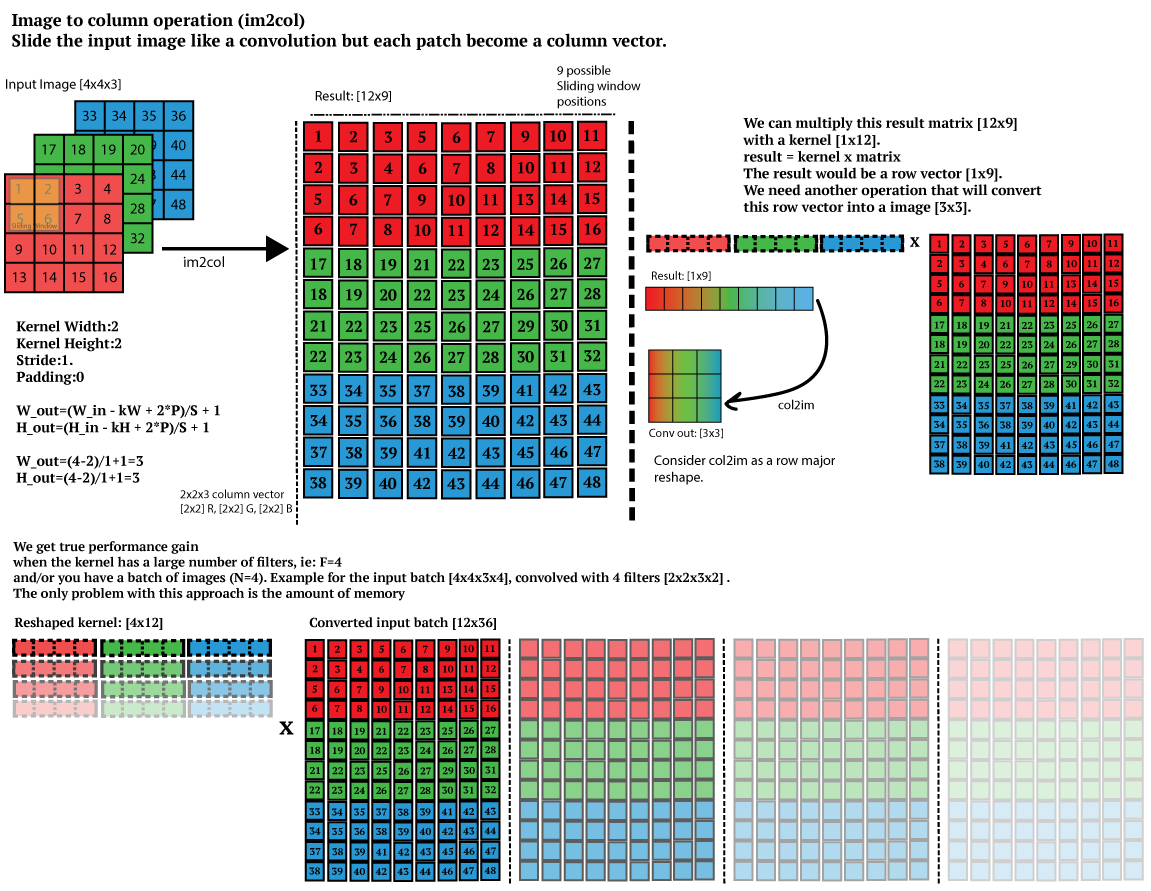
\includegraphics[width=0.85\textwidth]{im2col.png}
\caption{\textsf{im2col} algorithm scheme using a $2\times2$ filter on a image with 3 channels.
At the end of the \textsf{im2col} algorithm the \textsf{GEMM} is performed between weights and input image.
}
\label{fig:im2col}
\end{figure}
\end{center}

Taking into account what we have learned from the DNN models, we can re-formulate our problem using an efficient manipulation of the involved matrices to optimize the \textsf{GEMM} algorithm.
A direct convolution on an image of size ($W\times H\times C$), using a kernel mask of dimensions ($k \times k$), requires $O(WHCk^2)$ operations and thus several matrix products.
We can re-arrange the involved data to optimize this computation and evaluate a single matrix product: this re-arrangement is called \textsf{im2col} (or \textsf{im2row}) algorithm.
The algorithm is just a simple transformation which flats the original input into a bigger matrix, where each column carries all the elements which have to be multiplied for the filter mask into a single step\footnote{
  We work under the assumption that the weights matrix is already a flatten array and thus each row of the weights matrix represents the full mask.
}.
In this way we can immediately apply our \textsf{GEMM} algorithm on the full image.
In Fig.~\ref{fig:im2col} the main scheme of this algorithm is reported.
This algorithm optimizes the computational efficiency of the \textsf{GEMM} product but we have to store a lot of memory for the input re-organization in payback.

Using the mathematical theory behind the problem a third idea can arise using the well known Convolution Theorem: the Fourier transformation of our functions (that in this case are given by the input image and the weights kernel) can be reinterpreted into a simple matrix product in the frequency space.
This is certainly the most \quotes{physical} approach to solve this problem and probably the easier one since the Fourier Transformation is a well-known optimized algorithm, with several efficient implementations provided in literature.
One of the most efficient one is provided by the \textsf{FFTW} (\emph{Fast Fourier Transform in the West}) library~\cite{FFTW05}: \textsf{FFTW3} is an open source \textsf{Ansi-C} subroutine library for computing the Discrete Fourier Transform (DFT) in multiple dimensions, without constraints in input sizes or data types.
The library is not only computationally accurate, but it also provides an efficient parallel version for multi-threading applications.

A further implementation kind is given by linear algebra considerations (very closed to numerical considerations) and it is called \textsf{Coppersmith-Winograd algorithm}.
This algorithm was designed to optimize the matrix product and, in particular, to reduce the computational cost of its operations.
Suppose we have an input image given by just 4 elements and a filter mask with size equal to 3:

\begin{equation}
\mbox{img} = \left[\begin{array}{cccc} d0 & d1 & d2 & d3 \end{array}\right] \quad\quad \mbox{weights} = \left[\begin{array}{ccc} g0 & g1 & g2 \end{array}\right]
\end{equation}
\\
we can now use the \textsf{im2col} algorithm previously described and reshape our input image and weights into

\begin{equation}
\mbox{img} = \left[
\begin{array}{ccc}
d0 & d1 & d2 \\
d1 & d2 & d3
\end{array}
\right],
\quad\quad
\mbox{weights} = \left[
\begin{array}{c}
g0 \\
g1 \\
g2
\end{array}
\right]
\end{equation}
\\
given this data, we can simply compute the output as the matrix product of this two matrices.
The Winograd algorithm rewrites this computation as follow:

\begin{equation}
\mbox{output} = \left[
\begin{array}{ccc}
d0 & d1 & d2 \\
d1 & d2 & d3
\end{array}
\right]
\left[
\begin{array}{c}
g0 \\
g1 \\
g2
\end{array}
\right] = \left[
\begin{array}{c}
m1 + m2 + m3 \\
m2 - m3 - m4
\end{array}
\right]
\end{equation}
\\
where

\begin{equation}
\begin{aligned}
m1 = (d0 - d2)g0\quad\quad m2 = (d1 + d2)\frac{g0 + g1 + g2}{2}
\\
m4 = (d1 - d3)g2\quad\quad m3 = (d2 - d1)\frac{g0 - g1 + g2}{2}
\end{aligned}
\end{equation}
\\
where we can easily notice that the two fractions in $m2$ and $m3$ involve only weight quantities and thus they could be computed only one time for each filter (at each step).
Moreover, we have to manage $4$ \textsf{ADD} and $4$ \textsf{MUL} operations to calculate the $m_i$ quantities and $4$ other ADD to compute the result.
In doing normal matrix products we have to do $6$ \textsf{MUL} operations instead of $4$: the reduction of computational expensive \textsf{MUL} operations by a factor $1.5$x is very significant\footnote{
  A multiplication takes $7$ clock-cycles in a normal CPU while an add takes only $3$ clock-cycles.
}.
In this simple example we use a so-called $F(4, 3)$, i.e image of size $4$ and kernel of size $3$ which gives us $2$ convolutions.
More general formulations are $F(m\times m, r \times r)$ and if we use an image of size $4\times4$ and a kernel of size $3\times3$ we can compare the $16$ \textsf{MUL}s of the \textsf{Winograd} algorithm against the $36$ \textsf{MUL}s which are required by the normal matrix product ($2.25$x).
The \textsf{Winograd} efficiency has been widely proved for CNNs, especially when the kernel size is small.
In our \textsf{Byron} library we provide its implementation for kernel sizes equal to $3$, since the numerical generalization is not straightforward\footnote{
  We would also highlight that this formulation is valid only if we consider unitary strides.
}.

We tested the computational-time of each algorithm on different random images.
The tests were performed on a classical bioinformatics server (128~GB RAM memory and 2 CPU E5-2620, with 8 cores each) and we considered only kernel sizes equal to $3$ (\textsf{Winograd} constrain) varying input dimensions and number of filters.
In Fig.~\ref{fig:winograd_timing} we show the results of our simulations using the \textsf{im2col} values as reference\footnote{
  The \textsf{im2col} algorithm can be found in the major part of Neural Network library and it is also the only convolution function implemented in the \textsf{darknet} library, which is a reference for our work.
}.

\begin{figure}[htbp]
\centering
\def\svgwidth{0.8\textwidth}
\input{./img/winograd_timing.pdf_tex}
\caption{Time performances of different convolution algorithms: \textsf{im2col} (orange, reference), \textsf{FFTW3} (green, fast Fourier transformation using the \textsf{FFTW3} library) and \textsf{Winograd} (blue).
The values are normalized according to the \textsf{im2col} results since it is the most common convolution algorithm.
The tests were performed on different input sizes (width/height), keeping fixed the number of channels and the number of filters.
The tests were performed using a \textsf{C++} implementation of the three methods.
}
\label{fig:winograd_timing}
\end{figure}

In all our simulations we found a visible speedup using the \textsf{Winograd} algorithm against the other two algorithms: for small dimensions we obtained more than $5$x against the \textsf{im2col} and $25$x against the \textsf{fftw} implementation.
The worst algorithm is certainly the \textsf{fftw} one which, despite the efficient \textsf{FFTW3} parallel-library, is always more than $5$ times slower than the reference.
However, it is interesting notice how the \textsf{fftw} implementation is able to reach the best performances when the dimensions are proportional to powers of $2$, as expected from the mathematical theory behind the Discrete Fourier Transformation.

We can conclude that the \textsf{Winograd} algorithm is certainly the best choice when we have to perform a 2D convolution.
The payback of this method is given by the rigid constraints related to the mask sizes and strides: when it is possible it remains the best solution, but in all the other cases the \textsf{im2col} implementation is a relatively good alternative.
The efficiency of \textsf{Byron} library follows the efficiency of the \textsf{Winograd} algorithm, since the major part of layers in modern deep learning Neural Network models are Convolutional layers with sizes equal to $3$ and unitary strides.

%https://victorzhou.com/blog/intro-to-cnns-part-1/


\end{document}

\documentclass{standalone}

\begin{document}

\subsection[Pooling function]{Pooling function}\label{NN:pooling}

Output Neural Network feature maps often suffer of sensitivity on feature location in the input.
One possible approach to overcome this problem is to down sample the feature maps making the resulting feature map more robust to changes in the position.
Pooling functions perform this kind of down sample and they reduce the spatial dimension (but not depth) of the input.
Their use represents an important computational performance improver tool (less feature, less operations) and a useful dimensionality reduction method.
The reduction of feature quantity can also prevent over-fitting problems and it improves the classification performances.

Pooling layers are intrinsically related to Convolutional layers.
The analogy lives in the filter mapping procedure which produces the output in both methods.
While in the Convolutional layer we map a filter over the input signal and we apply a multiplication of the layer weights and the signal values, in the pooling layer we simply change the filter function keeping the same filter mapping procedure (see section~\ref{NN:convolutional} for more informations).
The input parameters of the method are the same of the Convolutional one: the input dimensions, the kernel size and (optional) the stride value.

The most common pooling layers are the Average Pool and the Maximum Pool.
The Average Pool layer performs a down sampling on the batch of images.
It slides a 2D kernel of arbitrary size over the image and the output is the mean value of the pixels inside the kernel.
In Fig.~\ref{fig:avgpool} are shown some results obtained by performing an average pool with different kernel sizes.
Also in this case this test was obtained using our NumPyNet library.

\begin{center}
\begin{figure}[htbp]
\centering
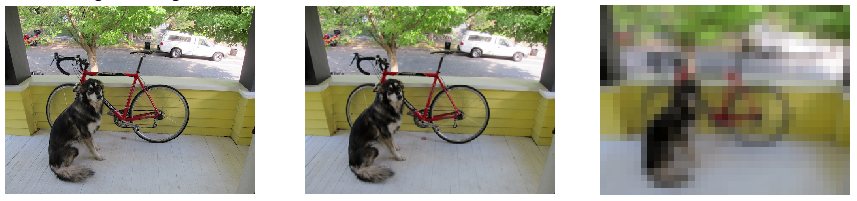
\includegraphics[width=0.85\textwidth]{avgpool_layer.png}
\caption{Average Pool functions applied on a testing image.
\textbf{(left)} The original image.
\textbf{(center)} Average Pool output obtained with a kernel mask $(3\times 3)$.
\textbf{(right)} Average Pool output obtained with a kernel mask $(30\times 30)$.
}
\label{fig:avgpool}
\end{figure}
\end{center}

If in the Convolutional layers a key role was played by the matrix product, in the Pooling layers we have to carefully manage the mapping operations to obtain optimal results.
In particular we would to show the efficient implementation provided into NumPyNet.

In the previous sections we introduced the \textsf{im2col} algorithm which is an efficient method to re-organize the input data.
The same algorithm can also be applied for Pooling layers and thus evaluate the Pooling function (avg, max, etc.) on each row of the re-arranged matrix.
The implementation of the \textsf{im2col} algorithm in Python requires the evaluation of multiple indexes using complex formulas.
Since the NumPyNet library was founded on the Numpy package we can provide an alternative implementation using the \textsf{view} functionality of the library.
A \textsf{view} of a given array is simply another way of viewing its data: technically that means that the data of both objects is shared and thus no copies are created.
In particular we can use the deeper functions of the Numpy package to create a re-organization of our data according to the desired output\footnote{
  The same technique was also used for the implementation of the Convolutional layer in the NumPyNet library.
}.
In the following code we show our implementation of the Average Pooling layer:

\lstset{style=snippet}
\begin{lstlisting}[language=Python, caption=NumPyNet version of AvgPool function, label=code:py_avgpool]
import numpy as np

class Avgpool_layer(object):

  def __init__(self, size=(3, 3), stride=(2, 2)):

    self.size = size
    self.stride = stride
    self.batch, self.w, self.h, self.c = (0, 0, 0, 0)
    self.output, self.delta = (None, None)

  def _asStride(self, input, size, stride):

    batch_stride, s0, s1 = input.strides[:3]
    batch,        w,  h  = input.shape[:3]
    kx, ky     = size
    st1, st2   = stride

    # Shape of the final view
    view_shape = (batch, 1 + (w - kx)//st1, 1 + (h - ky)//st2) + input.shape[3:] + (kx, ky)

    # strides of the final view
    strides = (batch_stride, st1 * s0, st2 * s1) + input.strides[3:] + (s0, s1)

    subs = np.lib.stride_tricks.as_strided(input, view_shape, strides=strides)
    # returns a view with shape = (batch, out_w, out_h, out_c, kx, ky)
    return subs

  def forward(self, input):

    self.batch, self.w, self.h, self.c = input.shape
    kx, ky = self.size
    sx, sy = self.stride

    input = input[:, : (self.w - kx) // sx*sx + kx, : (self.h - ky) // sy*sy + ky, ...]
    # 'view' is the strided input image, shape = (batch, out_w, out_h, out_c, kx, ky)
    view = self._asStride(input, self.size, self.stride)

    # Mean of every sub matrix, computed without considering the pad(np.nan)
    self.output = np.nanmean(view, axis=(4, 5))

\end{lstlisting}

A key role in this implementation is played by the \textsf{\_asStride} function: it returns a view of the original array in which all the masks are organized into a single list.
Using this data re-arrangement we can easily compute the desired pooling function (average in this example) according to the appropriated axes.
We would stress that no copies are produced during this computation and thus we can obtain a faster execution than other possible implementations (e.g \textsf{im2col}).

\end{document}

\documentclass{standalone}

\begin{document}


\section[BatchNorm function]{BatchNorm function}\label{batchnorm}

A common practice before the training of a Neural Network model is to apply some preprocessing to the input patterns.
A classical example is the normalization of training set, i.e it resembles a normal distribution with zero mean and unitary variance.
The initial preprocessing is useful to prevent the early saturation of non-linear activation functions (see section~\ref{activation}).
Moreover in this case we can ensure that all inputs are in the same range of values.

In a deep neural network architecture we can find the same problem also into the intermediate layers because the distribution of the activations is constantly changing during training.
This behavior produces a slowdown in the training convergence because each layer have to adapt itself to a new distribution of data in every training step (or \emph{epoch}).
This problem is also called \emph{internal covariate shift}.

A second problem arises from the heterogeneity of available input data.
If we tune the model parameters according to a given set of data which inevitably be limited we can meet problems during the generalization, i.e the validation of our model using new data, to new samples if they belongs to an equivalent but deformed distribution.
A classical example is given by the image detection: if we train a Neural Network model using gray-scale images we can find generalization problem using colored images.

BatchNorm function (Batch Normalization) allows to overcome these problems with a continuous rescaling of the Neural Network intermediate values during the training\footnote{
  The input data to feed the Neural Network model are commonly packed into a series of \emph{batches}, i.e small subsets of data.
  The BatchNorm function takes its name from this nomenclature and it processes each batch independently.
}~\cite{Sergey2015BatchNorm}.
In particular, the method processes the input of a given layer in order to fight the internal covariate shift problem removing the batch mean and normalizing by the batch variance:

$$
\mu_B = \frac{1}{m}\sum_{i=1}^{m}x_i \quad\quad {\sigma_B}^2 = \frac{1}{m-1}\sum_{i=1}^{m}(x_i - \mu_B)^2
$$
\\
and so the input data becomes:

$$
\hat{x_i} = \frac{x_i - \mu_B}{\sqrt{{\sigma_B}^2 + \epsilon}}
$$
\\
where we add an extra $\epsilon$ in the denominator for numerical stability\footnote{
  The floating point numbers into a computer have finite precision and the variance can underflow bringing to infinite values in the BatchNorm equation.
}.
After this common rescaling we also a apply a scaling-shift to previous results:

$$
y_i = \gamma\hat{x_i} + \beta
$$
\\
where the $\gamma$ and $\beta$ coefficients are left as variables to be tuned during the training (they are learned during training).
The updating rule of the function parameters ($\gamma$ and $\beta$) is given by the simple derivative of the previous function. % maybe insert backprop formulas
In this way we can ensure more stability of the extracted features~\cite{Lecun2000EffBackProp} during the training a faster convergence.

Since the BatchNorm function is became a sort of standard into a deep learning models an efficient implementation of this algorithm is essential to achieve the best computational performances.
We have also to take in count that the batch-normalization procedure is commonly performed after a fully-connected layer or a convolutional one.
Thus the best performances could be obtained merging the two functionality as much as possible as suggested in~\cite{AlexeyAB}.
In the next sections we will show our implementation of the algorithm and we discuss about the code optimization performed\footnote{
  The Byron library was inspired by the \emph{darknet} library provided by Redmon J. et al. and by its many branches.
  Despite in each implementation we can find the BatchNorm function, aware of the author, in any version we can find a right implementation of this function as standalone method.
  We have already highlighted that this normalization function can be efficiently joined to other function to increase the computational performances but in these case we have to different manage the dimensions of the involved arrays.
  A standalone implementation of the BatchNorm function required a rearrangement of its functions and it was provided into the Byron library.
  This was one of the various improvements provided by Byron against the other \emph{darknet}-like libraries.
}.

\end{document}

\documentclass{standalone}

\begin{document}


\section[Shortcut]{Shortcut function}\label{shortcut}


\end{document}

\documentclass{standalone}

\begin{document}


\section[Route]{Route function}\label{route}

\end{document}

\documentclass{standalone}

\begin{document}

% https://medium.com/@hirotoschwert/introduction-to-deep-super-resolution-c052d84ce8cf

\subsection[Pixel Shuffle]{Pixel Shuffle}\label{NN:shuffler}

Pixel Shuffle layer is one of the most recent layer type introduced in modern deep learning Neural Network.
Its application is closely related to the single-image super-resolution (SISR) research, i.e the ensemble techniques which aim at restoring a high-resolution image from a single low-resolution one (see section~\ref{SR:sr} for further details).

The first SISR Neural Networks start with a preprocessing of low-resolution images in input with a bi-cubic up-sampling.
Then the image, with the same dimensions of the desired output, feeds the model which aim to increase the resolution and fix its details.
In this way the amount of parameters and moreover the computation required by the training section increase (by a factor equal to the square of the desired up-sampling scale), despite the required image processing is smaller.
To overcome this problem a Pixel Shuffle transformation, also known as \emph{sub-pixel convolution}, was introduced~\cite{Wenzhe2016Shuffle}: in this work the authors proofed the equivalence between a regular transpose convolution, i.e the previous standard transformation to enlarge the input dimensions, and the sub-pixel convolution transformation without losing any information.
The Pixel Shuffle transformation reorganize the low-resolution image channels to obtain a bigger image with few channels.
An example of this transformation is shown in Fig.~\ref{fig:pixel_shuffle}.

\begin{figure}[htbp]
\centering
\def\svgwidth{0.7\textwidth}
\input{./img/pixel_shuffle.pdf_tex}
\caption{Pixel Shuffle transformation.
On the left the input image with $scale^2$ (:= 9) channels.
On the right the result of Pixel Shuffle transformation.
Since the number of channels is perfect square the output is a single channel image with the rearrangement of the original ones.
}
\label{fig:pixel_shuffle}
\end{figure}

Pixel Shuffle rearranges the elements of the input tensor expressed as $H \times W \times C^2$ to form a $scale \cdot H \times scale \cdot W \times C$ tensor.
This can be very useful after a convolution process, in which the number of filters chosen drastically increase the number of channels, to \quotes{invert} the transformation like a sort of \emph{deconvolution} function.

The main gain in using this transformation is the increment of computational efficiency of the Neural Network model.
The introduction of Pixel Shuffle transformation in the Neural Network tail, i.e after a sequence of small processing steps which increase the number of features, reorganize the set of features into a single bigger image, i.e the desired output in a SISR application.
The feature processing steps, which generally are faced on with convolutional layers, can be performed with smaller images in input and thus can be obtained faster since the up-scaling task will be performed by a single Pixel Shuffle transformation.

Despite this transformation has became a standard in super-resolution applications and thus it can be found into the most common deep learning libraries (e.g \emph{Pytorch} and \emph{Tensorflow}) a C++ implementation is hard to find.
Moreover, each library implements the transformation following its own data organization\footnote{
  The main difference between \emph{Pytorch} and \emph{Tensorflow} is related to the storage organization of the image.
  \emph{Tensorflow} has a \quotes{standard} input assessment as $H \times W \times C$.
  \emph{Pytorch} has a so-called channel-first implementation and so the input tensor is organized as $C \times H \times W$.
}.
For this reason we proposed in our libraries a dynamic version of the algorithm in C++ able to perform both versions of the algorithm.

The algorithmic implementation of the pixel-shuffle transformation is essentially a re-indexing of the input values.
While in a C++ implementation of the algorithm we could obtain the desired result inside a sequence of nested for loops playing with the loop indexes, for an efficient Python version we used a sequence of transposition and reshaping to rearrange the input values.
The following snippet shows the NumPyNet version of this algorithm.

\lstset{style=snippet}
\begin{lstlisting}[language=Python, caption=NumPyNet version of Pixel-Shuffle function, label=code:py_shuffle]
import numpy as np

class Shuffler_layer(object):

  def __init__(self, scale):

    self.scale = scale
    self.scale_step = scale * scale

    self.batch, self.w, self.h, self.c = (0, 0, 0, 0)

    self.output, self.delta = (None, None)

  def _phase_shift(self, input, scale):
    b, w, h, c = input.shape
    X = input.transpose(1, 2, 3, 0).reshape(w, h, scale, scale, b)
    X = np.concatenate(X, axis=1)
    X = np.concatenate(X, axis=1)
    X = X.transpose(2, 0, 1)
    return np.reshape(X, (b, w * scale, h * scale, 1))

  def _reverse(self, delta, scale):
    # This function apply numpy.split as a reverse function to numpy.concatenate
    # along the same axis also

    delta = delta.transpose(1, 2, 0)

    delta = np.asarray(np.split(delta, self.h, axis=1))
    delta = np.asarray(np.split(delta, self.w, axis=1))
    delta = delta.reshape(self.w, self.h, scale * scale, self.batch)

    # It returns an output of the correct shape (batch, in_w, in_h, scale**2)
    # for the concatenate in the backward function
    return delta.transpose(3, 0, 1, 2)

  def forward(self, input):

    self.batch, self.w, self.h, self.c = input.shape

    channel_output = self.c // self.scale_step # out_c

    # The function phase shift receives only in_c // out_c channels at a time
    # the concatenate stitches together every output of the function.

    self.output = np.concatenate([self._phase_shift(input[:, :, :, range(i, self.c, channel_output)], self.scale)
                                  for i in range(channel_output)], axis=3)

    self.delta = np.zeros(shape=self.out_shape, dtype=float)

  def backward(self, delta):

    channel_out = self.c // self.scale_step # out_c

    # I apply the reverse function only for a single channel
    X = np.concatenate([self._reverse(self.delta[:, :, :, i], self.scale)
                                      for i in range(channel_out)], axis=3)


    # The 'reverse' concatenate actually put the correct channels together but in a
    # weird order, so this part sorts the 'layers' correctly
    idx = sum([list(range(i, self.c, channel_out)) for i in range(channel_out)], [])
    idx = np.argsort(idx)

    delta[:] = X[:, :, :, idx]

\end{lstlisting}

The two functions \textsf{\_phase\_shift} and \textsf{\_reverse}\footnote{
  These function are \quotes{private} function of the object class.
}
produce the re-arrangement of the indexes according to the pixel-shuffle transformation and its inversion\footnote{
  During the back-propagation, in fact, we have to apply the reverse transformation to the gradient.
}
In the forward function we apply the \textsf{\_phase\_shift} to the sequence of channels (in the right order) and then we concatenate the results into a single tensor (output).
The backward function instead needs a re-ordering of channel sequence after the concatenation.

As told above, in the C++ implementation provided into the Byron library we can compute the desired re-indexing using a series of nested for loops.
An equivalent solution can be obtained also by the contraction of the loops into a single one using divisions to obtain the right indexes.
This solution was taken in count into the first version of the library but the amount of required divisions weights on the computational performances.
The division operations are the most computationally expensive operations in terms of CPU clock-time.
The old versions of OpenMP multi-threading library forced the users to spend time in the evaluation of the \quotes{loop-contraction} to obtain the better performances by a single parallel for loop.
The new features of OpenMP library provide the very powerful \emph{collapse} keyword which performs an automatic loop-contraction.
The keyword can be applied only with a series of independent and perfectly nested\footnote{
  Two for loops are perfectly nested if there are not other code lines between them.
}
for loops which is exactly our case.
Moreover we have not to take in care any thread concurrency trouble since the iterations, as the output indexes, are totally independent.
We widely used the \textsf{collapse} keyword in the Byron library to simplify the code and the function evaluation but the Pixel-Shuffle case is one of the most efficient one, since we could collapse six nested loops\footnote{
  In the Pixel-Shuffle we have to loop over batch, width, height, channels plus a couple of loops over the scale factor that we want to apply.
  In total we have to manage six dimensions that can be easily collapsed into a single one given by their product.
} (ref. \href{https://github.com/Nico-Curti/Byron/blob/master/src/shuffler_layer.cpp}{on-line}.

\end{document}

\documentclass{standalone}

\begin{document}

\subsection[Cost function]{Cost function}\label{NN:cost}

A machine learning algorithm is used to minimize or maximize a cost function.
In other words when we implement a machine learning algorithm we want to know how good is our result according to prior knowledge about the desired results.
So we have to establish a function ables to represent the error of our model.
This kind of function are commonly called \emph{error functions} or \emph{loss functions} or just simply \emph{cost function}.
In the previous sections we have shown many algorithms used into a Neural Network model and we have talked about how to update the functional parameters according to the evaluated error.
This error is provided by the cost function.

The cost function represents the final output of our Neural Network model so it is reasonable to talk about it at the end of this chapter.
There are many kinds of loss functions and there is not a particular one able to works with all kinds of data.
So we have to pay attention to chose the right one in our problems.
In particular we have to take in count the possible presence of outliers, the structure of our model, the computational efficiency of our algorithm and most of all the number of classes that we want to predict.
Broadly, we can classify the loss functions into two major categories: the classification losses and the regression losses.
In the first case we want to predict a finite number of categorical values (classes).
In the second case the prediction is performed on a series of continuous values.
Since in this work we are focusing only on classification problems we will only talk about the first case.

The most common cost function is given by the \emph{Mean Square Error} (MSE) or \emph{L2 loss} (very closed to the regularization function hinted at the end of \ref{NN:batchnorm}).
Its mathematical formulation is quite simple and it is given by

$$
MSE = \frac{\sum_{i=1}^{N}\left( y - t \right)^2}{N}
$$
\\
where we follow the nomenclature given in \ref{NN:perceptron} and $N$ is the number of output which is equivalent to the number of classes.
It is one of the most used cost function due to its simplicity either from a mathematical either from a numerical point of view.
The possible range of values ranged from 0 to $\infty$.
With MSE function the predictions which are far away from actual values are heavily penalized, due to the squaring.

A slight different function is given by the \emph{Mean Absolute Error} (MAE) or \emph{L1 loss} in which we replace the squaring with a module of the error.

$$
MAE = \frac{\sum_{i=1}^{N}|\left( y - t \right)|}{N}
$$

With MAE we loose the information about the error direction (preserved by the squaring in MSE) and just simply evaluate the absolute value of it.

The main differences between these two functions can be summarized as follow: using the MSE function we can easily solve the problem but the MAE function is more robust against possible outliers.
Despite both functions reach the minimum in a perfect classification configuration (error equal to zero), in presence of outliers we have to manage with large differences in the numerator of the function.
With large differences, the square values are greater than the absolute values but while the MSE tries to adjust its performance to minimize those cases, the other samples pay the higher cost.

A problem related to the MAE function arises during the gradient evaluation.
Its gradient, in fact, is the same throughout, which means that we will have large gradient values also with small differences which is a worse configuration during the training.
A simple possible workaround is to introduce a shrinking parameter, given by a dynamic learning rate, when we move closer to the minimum.

When we have to manage multi-class problems there are other common cost functions based on likelihood scores.
The simpler one is the \emph{Cross Entropy loss} or \emph{Log loss}:

$$
CrossEntropyLoss = -(y\cdot\log(t) + (1 - y)\cdot\log(1 - t))
$$

This function just multiply the log of the actual predicted probability by the ground truth class.
In this way when we have two classes (e.g $t \in [0, 1]$) we can alternatively nullify the two parts of the function\footnote{
  When the actual label is equal to 1, i.e $y=1$, the second half of the Log Loss function disappears whereas in case of actual label is equal to 0 the first half is null.
}.
In this way the loss function heavily penalizes the predictions that are confident but wrong.
This function works with binary classification problems where the output classes are binned in $[0, 1]$.
For this reason the output of the model must be constrained into the $[0, 1]$ domain and thus a proper activation function should be provided.
Classically this loss function is used jointly to the sigmoid activation (ref.~\ref{NN:activation}) which constrains the output of the model in the desired interval.
For this reason in our implementation of the algorithm we chose to merge the sigmoid function and the Log Loss function into a single object\footnote{
  We also try to prevent wrong uses of this loss function for laypersons.
  This implementation was already suggested by the \emph{darknet} library so we simply propagate it in our implementations.
}.

A last duty to mention loss function is the extension of the Log loss to multiple classes, the so-called \emph{Categorical Cross Entropy Loss}.

$$
CategoricalCrossEntropyLoss = -\sum{i=1}^{N}\left( y\cdot\log(t) \right)
$$

This function generalized the previous one for multiple-classes, i.e for problems where the correct output can be only one.
The loss compare the distribution of the predictions, i.e output of the model, with the prior known distribution.
In this way only the probability of the true class will be 1 and all the other classes will be set to 0.
Also in this case we have to pay attention to the output of our model which is intended as a probability value ranging in $[0, 1]$.
In particular this function commonly works jointly to a softmax activation function.
As in the previous case we chose to implements this loss function in a separated object associated to the softmax transformation.

Many other loss function can be mentioned to overcome different kind of problems.
The list of presented loss function was related to the implementation of the \emph{darknet}-like library which are ported also into the NumPyNet and Byron libraries, i.e either in Python and C++.
NumPyNet and Byron libraries also provided a wider list of loss functions to improve the usability of them and improve their computation (and fixed some \emph{darknet} issues).
A full list of available loss functions can be found in the \href{https://github.com/Nico-Curti/Byron/blob/master/src/cost_layer.cpp}{on-line} version of the libraries with a list of easily visual examples.

A further improvements was given from a numerical point-of-view: many mathematical formulas needs expensive math operations as logarithms and trigonometric functions.
An efficient (but approximated) math formulas was implemented both in the C++ and Python to reach faster computational performances.
These numerical math operations are widely used into the Byron library to increase the performances despite their used can be turned off by user at compile time in Byron.
The full set of functions, in fact, is enclosed into a \textsf{macro} definition (\textsf{\_\_fmath\_\_}) that can be enabled at compile-time.

A classical example of this faster math operation is given by the \emph{fast inverse square root} algorithm, firstly introduced in 1999 in the source code of \emph{Quake III Arena}, a first-person shooter video game.
The method is based on a Newton algorithm which can be stopped at the desired precision order: less precision is associated to faster execution, obviously.
In our \textsf{fast math} implementation we provide a set of Newton algorithms associated to the most common mathematical operations, like \textsf{exp}, \textsf{log}, \textsf{sqrt} and so on.
We tested these implementations against the common standards (Numpy package for Python and \textsf{std::} for C++) and we compare the time execution performances (we required a precision of at least $10^-4$).
The obtained results are shown in Fig.~\ref{fig:fmath} where we normalized the execution time taking Numpy implementation as reference.

\begin{figure}[htbp]
\centering
\def\svgwidth{0.8\textwidth}
\input{./img/fmath_timing.pdf_tex}
\caption{Time performances of standard mathematical operations implemented through Newton approximations.
We compare the results obtained with the Numpy library (blue, reference) and the standard C++ library (\textsf{CMath}) to their equivalent into the custom \textsf{FMath} version.
In the comparison we have to take in mind that the Numpy library is based on a C++ wrap and that the Python version of the \textsf{FMath} is written in pure Python language.
In all the cases the \textsf{FMath} version of the functions performs better or at-least-equal to the standard one.
}
\label{fig:fmath}
\end{figure}

As can be see all the results obtained by the \textsf{fast math} algorithms are faster or at least equals to the standard ones.
The C++ version of the \textsf{fast math} is certainly the better choice for an efficient implementation of the algorithms in all the cases and it is interesting to notice how some functions (\textsf{pow2} and \textsf{log10}) are drastically slower in C++ than in Python, despite the intrinsic overhead of the Python language.
This is probably due to particularly optimizations performed by the Numpy package in the implementation of these special cases: if we compare those functions to the general ones (\textsf{pow} and \textsf{log}), in fact, the results confirm the efficiency of the C++ language.

These results highlight the importance of code testing before release it: we have to pay always attention in writing a code and query also the standard choices.


\end{document}


\documentclass{standalone}

\begin{document}

\section[Object Detection]{Object Detection}\label{obj_detection:obj}

Object detection is one of the larger deep learning sub-discipline, especially when we talk about Neural Network models.
This kind of problems aim to identify single or multiple objects into a picture or video stream.
The possible applications of these tools are everywhere these days and they involve object tracking, video surveillance, pedestrian detection, anomaly detection, people counting, self-driving cars or face detection and the list goes on.

There are many machine learning and deep learning techniques proposed during the years about this topic and each one has its own pros and cons.
The most prominent and moder techniques involve the use of very deep Neural Network models, with a huge amount of parameters to tune.
The most famous ones are probably the Faster R-CNN (\emph{Faster Region Convolutional Neural Network})~\cite{ren2015faster} and its \quotes{evolution} into the YOLO (\emph{You Only Look Once}) model~\cite{redmon2015look, redmon2016yolo9000, redmon2018yolov3}.

The R-CNN models are one of the state-of-art CNN-based deep learning object detection model and their evolution into Fast R-CNN tries to improve their speed.
The standard approach for object detection is based on moving a \emph{sliding window} to search in every position of the image the objects.
However, the intrinsic problems of these kinds of methods are the window dimensions and the large computation required to map with multiple window sizes the full image.
Different objects, or even the same kind of objects, could have different aspect ratios and sizes in relation to the position of the camera which captured the image or to their distances.
R-CNN models try to overcome these problems generating about \numprint{2000} region proposals, i.e bounding boxes, and applying to each one a image classification procedure, using a standard CNN.
Finally, each detected region can be refined using a regression approach.

A Faster R-CNN model is based on the same idea but, instead of feeding the bounding boxes to the CNN, it feeds the input image to the CNN to generate a convolutional feature map.
Starting from this feature map we can easier identify the region of proposals (Region Proposal Network) and warp them into squares.
The list of these regions are then reshaped using a Polling layer and processed by a fully connected layer.
The advantages of Faster R-CNN are thus visible: we do not need to feed \numprint{2000} region proposals to the CNN every time, but the feature map is generate once per image using the convolution operation.
In this way we can also separate the feature map creation to the selective search algorithm.

A key role on these models is given by the \emph{anchor} concept: an \emph{anchor} is essentially a box and it identifies the shape of a portion of the input image at different scale levels.
The CNN feature map feeds the Region Proposals Network which uses a sliding window over it, generating $k$ anchor boxes.
These boxes are certainly fewer than the previous cited \numprint{2000} windows.

A breakthrough idea on the real-time object detection was the introduction of the YOLO model.
The model was developed by Redmon et al. at Washington University and it is probably the state-of-art on object detection, especially for its very incredible speed (it can reach 45 FPS on modern GPUs!).
Certainly it is the faster method publicly available, but its popularity is also due to its innovative strategy in object detection.
Despite all the other algorithms use regions to localize the object into the image, the YOLO network does not look at the complete image but only on a parts of it, which has the higher probability to contain an object.
In YOLO a single CNN predicts the bounding boxes and the class probabilities of them.
YOLO slits a single image into a $S\times S$ grid and on each grid $m$ bounding boxes are taken.
For each of them, the CNN outputs a class probability and offset values.
Finally, these bounding boxes are filtered according to their probability and a chosen threshold.

One of the most bigger limitation of this model is that it struggles with small objects.
This is due to the spatial constraints of the algorithm.
Fortunately, in the previous sections we have already discussed on how we can overcome this kind of problem using Super Resolution.
In the next section we will discuss about further characteristics of the YOLO model and about its implementation into the \textsf{Byron} library, considering its efficiency against the original implementation.
Finally, we will join the efficiency of the previous Super Resolution models to the performances of our optimized implementation of YOLO.


%Introduction on the image classification and detection with Yolo architecture.
%Implementation in Byron with description of performances against darknet (original implementation).
%Focus on performances (time, memory, cpu).


\end{document}


\documentclass{standalone}

\begin{document}

\section[Super Resolution]{Super Resolution}\label{SR:sr}

\begin{figure}[htbp]
\def\svgwidth{0.5\textwidth}
\input{./img/sr_wow.pdf_tex}
\quad
\def\svgwidth{0.465\textwidth}
\input{./img/sr_wow2.pdf_tex}
\caption{Single Image Super Resolution.
Between the red lines the super resolved version of the original image.
}
\label{fig:sr_wow}
\end{figure}

The Super Resolution (SR) is a slight novel technique based on Neural Network models which aims to improve the spatial resolution of a given image\footnote{
  The best-known \quotes{implementation} of Super Resolution concerns the microscopy super-resolution.
  In this work we are focusing on algorithms and numerical implementations so we will talk about the numerical counterpart of this technique, totally ignoring the original \quotes{hardware} version.
}.

The first SR methods on digital images estimate the high frequency information of the images, starting from a series of low-resolution (LR) patches and their high-resolution (HR) counterparts.
These patches (ROIs of the LR image commonly smaller than $50\times50$) were extracted after an edge enhancement procedure or a simple 2D Fourier transformation, which extracts the high frequency information.
Collecting these patches an \quotes{association dictionary} between LR and HR was created.
This dictionary was used to learn the correct associations between LR and HR and then applied on new images.
The images considered were of the same dimensions in these firstly applications, i.e the purpose was only to improve the spatial resolution of the image without changing the sampling step.

The idea of use neural network models and in particular convolution functions to face this problem was born in 2014 at the Engineering University of Honk Kong, due to the large popularity of these models during those years.
The increasing computational power allowed to create automatic models able to learn the LR-HR associations without any dictionary.
In this year the SRCNN model~\cite{SRCNN} arises, a three-layer neural network able to learn a large ensemble of features to reproduce the desired associations.
The first layer aimed to extract the LR patches from the input image; the second layer produces the association between the LR patches and the tuned HR ones; the last layer reorganized the HR patches ensemble produced into a single HR image, i.e the output.

From this starting implementation many improvements was performed in this research field, but the fundamental idea is not changed.
Modern models simply have a greater number of layers, due to the increasing computational power availability, and they use appropriated workaround to overcome the (large-)parameters tuning problem.

In the next sections we will show the super resolution technique step-by-step starting from the image pre-processing up to the most modern algorithmic solutions.
At the end of this chapter the \textsf{NumPyNet} and \textsf{Byron} implementations of some modern models will be presented and applied over biomedical images.

%Introduction on Super Resolution problem with focus on state-of-art neural network architecture.
%Description of the Byron implementation and application on NMR data with the most common measurements.
%Super-resolution allows better detection!


\end{document}

\documentclass{standalone}

\begin{document}

\subsection[Resampling]{Resampling}\label{SR:downsampling}

Up to now we have talked about neural network models as classification algorithms.
In the SR problem we have no classes but the desired output is a image.
This behavior is often hard to digest but it does not change anything about the previous consideration.
The only change will be related to the size of the neural network and its amount of parameters that could drastically increase due to the larger output required.
Lets start from the beginning: to feed a super-resolution model we have to use a series of prior-known LR-HR image association.
In the real life we always have a series of images, typically LR images, and we want to enlarge the resolution of them, i.e enlarge the spatial dimensions of the input image, to better see some particulars or just to create an output without artifacts or evident pixel grains.
If we consider these series of images as the HR one we can easily down-sample them without particular troubles\footnote{
  Ignoring particular cases the hardest step is always to enlarge the image resolution and not the inverse step.
}.
This re-sampling will introduce a aliasing factor that our model should learn to nullify.
The number of model parameters is typically around the $10^7$ so if we introduce any filtering process (degradation) in the input image the model will be able to overcome also these problems.

Starting from these considerations we can down-sample our images by a desired scale factor: common scale factor are between 2 and 8 and in this work we will refer to a scaling equal to 4.
A crucial role is played by the re-sampling (or down-sampling) algorithm chosen for the artificial image degradation.
Any down-sampling algorithm, in fact, loose part of the original information by definition.
Thus we can facilitate the learning choosing a lossless one but in this way we will loose in generalization (the model will not learn how to overcome some cases), or we can apply a drastic down-sample technique and achieve better performances later.

The simpler down-sampling algorithm is given by a \emph{nearest interpolation}.
This algorithm pass a kernel mask over the image and it substitutes each pixel mask to their average\footnote{
  The inverse (up-sampling) interpolation simply replicates each pixel in each dimension by a number equal to the scale factor.
}.
This procedure can be achieved using a \emph{Pooling} algorithm (in particular an AveragePooling) (ref.~\ref{NN:pooling} for further informations) for the down-sample or we can use an UpSample layer.
The UpSample function is commonly related to GAN (Generative Adversarial Networks) models in which we have to provide a series of artificial images to a given Neural Network but it is a function which can be introduce inside a Neural Network model to rescale the number of features.
We mention it in this section since it is not intrinsically related to a Neural Network model but it could be use as image processing technique.

We provide an implementation of this algorithm either in \textsf{NumPyNet} either in \textsf{Byron} library using different techniques.
The UpSample function inside a Neural Network model has to provide both up- and down- sampling technique since one is used in the forward function and its inverse during the back-propagation.
To achieve this function in \textsf{NumPyNet} we can use a series of reshapes and striding on the input matrix as shown in the following snippet.

\lstset{style=snippet}
\begin{lstlisting}[language=Python, caption=NumPyNet version of Upsampling function, label=code:py_upsample]
import numpy as np
from numpy.lib.stride_tricks import as_strided

class Upsample_layer(object):

  def __init__(self, stride=(2, 2), scale=1., **kwargs):

    self.scale = float(scale)
    self.stride = stride

    if not hasattr(self.stride, '__iter__'):
      self.stride = (int(stride), int(stride))

    assert len(self.stride) == 2

    if self.stride[0] < 0 and self.stride[1] < 0: # downsample
      self.stride = (-self.stride[0], -self.stride[1])
      self.reverse = True

    elif self.stride[0] > 0 and self.stride[1] > 0: # upsample
      self.reverse = False

    else:
      raise NotImplementedError('Mixture upsample/downsample are not yet implemented')

    self.output, self.delta = (None, None)

  def _downsample (self, input):
    batch, w, h, c = input.shape
    scale_w = w // self.stride[0]
    scale_h = h // self.stride[1]

    return input.reshape(batch, scale_w, self.stride[0], scale_h, self.stride[1], c).mean(axis=(2, 4))

  def _upsample (self, input):
    batch, w,  h,  c  = input.shape     # number of rows/columns
    b,     ws, hs, cs = input.strides   # row/column strides

    x = as_strided(input, (batch, w, self.stride[0], h, self.stride[1], c), (b, ws, 0, hs, 0, cs)) # view a as larger 4D array
    return x.reshape(batch, w * self.stride[0], h * self.stride[1], c)                                     # create new 2D array

  def forward(self, input):
    self.batch, self.w, self.h, self.c = input.shape

    if self.reverse: # Downsample
      self.output = self._downsample(input) * self.scale

    else:            # Upsample
      self.output = self._upsample(input) * self.scale

    self.delta = np.zeros(shape=input.shape, dtype=float)

  def backward(self, delta):
    if self.reverse: # Upsample
      delta[:] = self._upsample(self.delta) * (1. / self.scale)

    else:            # Downsample
      delta[:] = self._downsample(self.delta) * (1. / self.scale)


\end{lstlisting}

Thus the down-sampling algorithm is obtained reshaping the input array according the two scale factors (\textsf{strides} in the code) along the two dimensions and computing the mean along these axes.
Instead the up-sample function use the stride functionality of the \textsf{Numpy} array to rearrange and replicate the value of each pixel in a mask of size \textsf{strides}$\times$\textsf{strides}.

The same functionality can be obtained in the \textsf{C++} version of the code provided by the \textsf{Byron} library in which we compute the right indexes along a nested sequence of for loops (ref. \href{https://github.com/Nico-Curti/Byron/blob/master/src/upsample_layer.cpp}{on-line}).
We have to take in care the summation reduction provided by the down-sampling according to the thread concurrency: in this case we can not generalize the loop collapsing to the full set of lops but we have to separately manage the summation in a sequential section.

A more sophisticated interpolation algorithm, which reduce the loosing informations, is provided by the \emph{bicubic interpolation}.
The re-sampling algorithm interpolate the information provided by the nearest pixels using a cubic function.
Given a pixel, the interpolation function evaluates the 4 pixels around it applying a filter given by the equation:

$$
k(x) = \frac{1}{6} \left\{ \begin{array}{rc}
  (12 - 9B - 6C) |x|^3 + (-18 + 12B + 6C) |x|^2 + (6 - 2B)           & \mbox{if}        |x| < 1 \\
  (−B − 6C) |x|^3 + (6B + 30C) |x|^2 + (−12B − 48C) |x| + (8B + 24C) & \mbox{if} 1 \leq |x| < 2 \\
  0                                                                  & otherwise                \\
  \end{array}
  \right.
$$
\\
where $x$ identify each pixel below the filter.
Commonly values used for the filter parameters are $B=0$ and $C=0.75$ (used by \textsf{OpenCV} library) or $B=0$ and $C=0.5$ used by \textsf{Matlab}\footnote{
  In this case the filter is also called Catmull-Rom filter.
}.
Despite this function was also implemented in the most common library in \textsf{Python} we provide an efficient multi-threading implementation in the \textsf{Byron} library.

Equivalent performances could be achieved using a generalized version of the bicubic filter which use the 8 positions mask around each pixel, the so called Lanczos filter.
Also this function was provided into the \textsf{Byron} library.

To better understand the told above functions we can consider their application on the simple image given in Fig.\ref{fig:resampling}.

\begin{figure}[htbp]
\centering
\def\svgwidth{\textwidth}
\input{./img/up_down_sampling.pdf_tex}
\caption{Re-sampling image example.
\textbf{(left)} The original image.
\textbf{(up right)} The down-sampled blue-ROIs using different interpolation algorithm (Nearest, Bicubic and Lanczos, respectively).
We use a scale factor equal to 2 (half size in down-sampling and double size in up-sampling).
The Lanczos interpolation is the lossless algorithm but from a qualitative point-of-view the result is the quite the same of the bicubic one.
\textbf{(down right)} The up-sampled red-ROIs using the same interpolation algorithm of the upper row.
Also in the Up-sampling the Lanczos and bicubic algorithms produces equal qualitative results.
The Nearest algorithm produces the worse results in both up- down- cases.
}
\label{fig:resampling}
\end{figure}

In the figure the three algorithms were applied over the same image to highlight the differences against the down-sampling and up-sampling.
The nearest interpolation algorithm produces always the worse results both in up-sampling and down-sampling.
In the bicubic and Lanczos down-sampling we can better appreciate the \quotes{preservation} of the line shapes that are lost using the Nearest algorithm.
The result obtained by bicubic and Lanczos are quite similar in both cases but the computational cost of the Lanczos algorithm is greater than the bicubic one.
This is the reason why the bicubic interpolation is the most used technique for image resizing with a balance between computational cost and qualitative results.
In our implementation of SR algorithms we chose to use the bicubic interpolation for those reasons.

The aim of SR algorithm is to overcome these results and obtain a better quality image either from an optical point-of-view either from a mathematical one.
Until now we are considering the quality of the digital image only from a qualitative point-of-view.
In the next section we will introduce some useful mathematical scoring to numerically evaluate the image quality.

\end{document}

\documentclass{standalone}

\begin{document}

\section[Image Quality]{Image Quality}\label{SR:quality}

The most common image quality evaluator is given by our eyes.
This is true also for SR problems: the final purpose still remain to obtain images that are better visible for human eyes, the so called \emph{visual loss}.
We can however provide some mathematical formulas which allows to quantitative evaluate the image quality.
In both cases we need to establish a relation between the original image and the produced one.
Thus we can formulate a quality score only with a reference image.
In SR problems, or more in general in up-sampling problems, we can compare the original HR image with the image obtained by the output of our model.
In this way our quality score will be a measure of similarity between the two images.

The simple similarity score can be obtained evaluating the peak-signal-to-noise-ratio (PSNR).
This quantity is commonly used to establish the compression lossless of an image and it can be computed as

$$
PSNR = 20 \cdot \log_{10}\left( \frac{\max(I)}{\sqrt(MSE)} \right)
$$
\\
where $\max(I)$ is the maximum value which can be taken by a pixel in the image (in general it will be 1 or 255 depending on the image format chosen) and $MSE$ is the Mean Square Error (ref.~\ref{NN:cost}) between the original image and the reconstructed one.
The MSE for an image can be computed as:

$$
MSE = \frac{1}{WH} \sum_{i=1}^{W}\sum_{j=1}^{H} \left( I(i, j) - K(i, j) \right)^2
$$
\\
where $W$, $H$ are width and height of the two images and $I$, $K$ are the original and reconstructed images, respectively.

In other words the PSNR is the maximum power of the signal over the background noise.
It is expressed in decibel (dB) because the image values ranging in a wide interval and the logarithmic function rearrange the domain.
Thus we can conclude that high PSNR values are associated to a good reconstruction of the original image.

The PSNR is probably the most common quality score~\cite{psnr_ssim} but it does not always related to a qualitative visual quality.
Despite it is commonly used as loss function for SR models.

\begin{table}[htbp]
\centering
\begin{tabular}{lccc}
\hline \rowcolor{darkgrayrow}
         & Nearest       & Bicubic        & Lanczos  \\
\hline
PSNR     & 25.118        & 27.254         & 26.566   \\
SSIM     &  0.847        &  0.894         &  0.871   \\
\hline
\end{tabular}
\caption{Image quality scores: PSNR (peak-signal-to-noise-ratio) and SSIM (Structural SIMilarity index).
The values are computed on the image shown in Fig.~\ref{fig:resampling}.
The original image was down-sampled using a Lanczos algorithm and then re-up-sampled using three different algorithms: nearest, bicubic and Lanczos interpolations.
For each interpolation algorithm the PSNR and SSIM was evaluated.
As expected the highest scores were obtained using the bicubic algorithm while the worst reconstruction is performed by the nearest algorithm.
}
\label{tab:psnr}
\end{table}

Considering the series of images shown in Fig.~\ref{fig:resampling} we can evaluate the PSNR score starting from a down-sampled image.
Taking the down-sampled image obtained with the Lanczos algorithm we can compare the original image with their up-sampled version given by the three methods (ref. Tab.~\ref{tab:psnr}).
As expected, the lowest PSNR value is achieved by the nearest interpolation method while the best performances are obtained by the bicubic algorithm.
This confirm the wider use of bicubic method in image processing applications.
Moreover we have to take in account that an increment of 0.25 in PSNR value correspond to a visible improvement for human eyes.

A more advanced quality score, commonly used in super resolution image evaluation, is given by the \emph{Structural SIMilarity index} (SSIM).
The SSIM aims to mathematically evaluate the structural similarity between two images taking into account also the visible improvement seen by human eyes.
The SSIM function can be expressed as

$$
SSIM(I, K) = \frac{1}{N}\sum_{i=1}^{N} SSIM(x_{i}, y_{i})
$$
\\
where $N$ is the number of arbitrary patches which divide the image\footnote{
  Patch dimensions commonly used are $11\times11$ or $8\times8$.
}
For each patch the SSIM is computed as

$$
SSIM(x, y) = \frac{(2\mu_x\mu_y + c_1)(2\sigma_{xy} + c_2)}{ ({\mu_x}^2 + {\mu_y}^2 + c_1)({\sigma_x}^2 + {\sigma_y}^2 + c_2) }
$$
\\
where $\mu$ and $\sigma$ are the means and variances of the images, respectively, and $\sigma_{xy}$ represents the covariance.
The $c_1$ and $c_2$ parameters are fixed to avoid mathematical divergence.
Also in this case higher value of SSIM corresponds to high similarity between the original image and the reconstructed one.

Based on the previous equation we can highlight a link with the pooling functions discussed in~\ref{NN:pooling}.
Also in this case, in fact, we works with a window/kernel moved along the image which applies a mathematical function on the underlying pixels.
This equivalence suggests an easy implementation of this method with slight modifications of the previous code.

The evaluation of SSIM quality score on the previous up-sampled images (ref. Fig.~\ref{fig:resampling} and Tab.~\ref{tab:psnr}) confirms the results obtained by the PSNR.
Also in this case the worst reconstruction is obtained by the nearest algorithm while the highest SSIM is obtained by the bicubic algorithm.
The gap between SSIM values is smaller than PSNR ones but this is due to the different domains of the two functions.

\end{document}

\documentclass{standalone}

\begin{document}

\subsection[Super Resolution Models]{Super Resolution Models}\label{SR:wdsr}

\begin{center}
\begin{figure}[htbp]
\centering
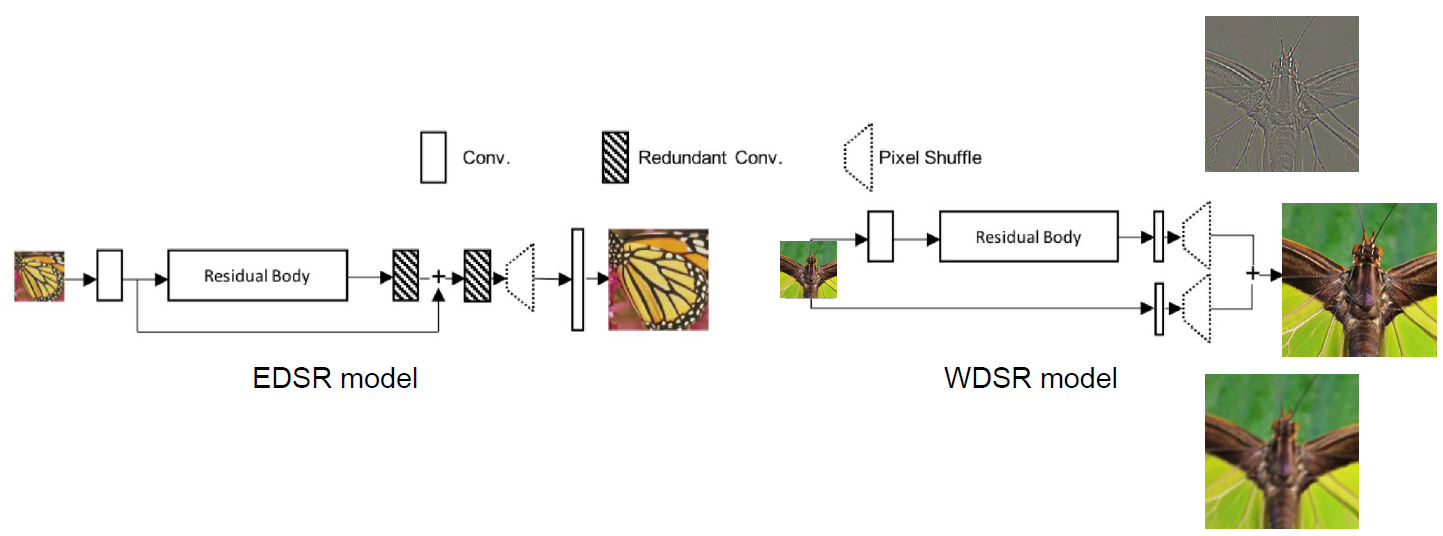
\includegraphics[width=0.85\textwidth]{SR_models.png}
\caption{Super Resolution models analyzed in this word.
\textbf{(left)} EDSR model.
The model is a modified version of the ResNet architecture designed for SISR applications.
The architecture is made by a sequential CNN framework which processes the input image.
The EDSR has more than 43 million of parameters in total.
\textbf{(right)} WDSR model.
The model is the updated version of the EDSR one.
The model optimizes its numerical efficiency using a different approach in the analysis of low- and high-frequency components in the input image.
the WDSR has slight more than 3.5 million of parameters, less than 10\% of the EDSR model.
}
\label{fig:sr_models}
\end{figure}
\end{center}

There were different kind of models proposed for image Super Resolution purposes but in this work we focused only on two of them.
Both are based on deep learning Neural Network models and they became famous in the research community since they both won the last NTIRE editions, 2017 and 2018 respectively.

\begin{table}[htbp]
\centering
\begin{tabular}{lccc}
\hline \rowcolor{darkgrayrow}
                         &  Channels     & Filter     & Number of    \\
\rowcolor{darkgrayrow}
Layer                    & input/output  & dimensions & Parameters   \\
\hline
Conv. input              & 3/256      & $3\times3$   & 6912    \\
Conv. (residual block)   & 256/256    & $3\times3$   & 589824  \\
conv. (pre-shuffle)      & 256/256    & $3\times3$   & 589824  \\
Conv. (upsample block)   & 256/1024   & $3\times3$   & 2359296 \\
Conv. output             & 256/3      & $3\times3$   & 6912    \\
\hline
\end{tabular}
\caption{EDSR model scheme summary.
We highlight the number of parameters of each macro-block.
The total number of parameters of this model is given by the sum of the values in the last column (more than 3 million of parameters).
}
\label{tab:edsr}
\end{table}

The first model is called EDSR (\emph{Enhanced Deep Super Resolution}) and was firstly proposed at the NTIRE challenge in 2017~\cite{Agustsson_2017_CVPR_Workshops}.
The EDSR model structure could be broadly summarized as an updated version of the SRResNet model which is already a modified version of the classical ResNet (standard CNN based on multiple residual blocks).
The major updates concern a series of optimization to improve the training speed and the quality of the output image.
In particular, the batch normalization steps are removed to improve the algorithm speed: it was proved that in low-level vision tasks as the super resolution one, i.e without complex evaluations as object detection, a wide and dynamic range of outputs can be useful~\cite{edsr}.
A scheme of the EDSR architecture is shown in Fig.~\ref{fig:sr_models}(a) and the full set of parameters are reported in Tab.~\ref{tab:edsr}: the EDSR model has more than 43 million of parameters in total.

A first convolutional layer takes the LR image which is processed using 256 filters.
Then a set of 32 residual blocks (convolution with 256 filters + ReLU activation + convolution with 256 filters + linear combination of the output with the input) process the feature map.
The tail of the architecture is made by an up-sample block which re-organize the pixels using a series of convolution and pixel-shuffle functions.
The up-sampling follows the scale factor imposed: the model increases the spatial resolution of the image by a fixed scale factor (x2 and x4 in our applications) and each pixel-shuffle application is equivalent to a x2 in the output sizes\footnote{
  It is straightforward that adding multiple up-sampling blocks and thus pixel-shuffle functions we can train the model according to every desired upscale.
}.

The first convolutional layer extracts the low frequency components of the input image which will be combined to the output of the residual blocks at the end of the model.
The residual blocks with their relative convolutional layers extract the feature map and the high frequency informations into the LR image: in this way the low- and high-frequency components are \quotes{independently} analyzed by the model and then re-combined in the output.
The last set of up-sampling blocks simply reshape and reorganize the extracted informations according to the desired sizes.

The large amount of filters of the up-sampling blocks and the input dimensions drastically affect the computational performances of the model: we numerically evaluated that the most time spent by the processing is related to the tail of the model and thus to the up-sampling blocks.

The second analyzed and implemented model is the WDSR (\emph{Wide Deep Super Resolution}) model which won the NTIRE challenge in 2018~\cite{wdsr}.
The WDSR model is a modified version of the EDSR one.
The improvements principally concern two aspects: the network structure and the residual blocks.

As shown in Fig.~\ref{fig:sr_models}(b), the WDSR simplifies the network architecture removing the convolutional layers after the pixel-shuffle ones.
Moreover, if the EDSR applies a x2 up-sampling every pixel-shuffle layer, in the WDSR a single pixel-shuffle function performs a x4 up-sampling.
This update drastically reduce the computational time and the amount of parameters.
Furthermore, the combination between low- and high- frequency components in this case are processed separately (two different branches) and only at the end they are re-combined (ref. Fig.~\ref{fig:sr_models}(b)).

\begin{table}[htbp]
\centering
\begin{tabular}{lccc}
\hline \rowcolor{darkgrayrow}
                            &  Channels     & Filter     & Number of    \\
\rowcolor{darkgrayrow}
Layer                       & input/output  & dimensions & Parameters   \\
\hline
Conv. input 1               & 3/32       & $3\times3$   & 864     \\
Conv. 1 (residual block)    & 32/192     & $3\times3$   & 55296   \\
conv. 2 (residual block)    & 192/32     & $3\times3$   & 55296   \\
Conv. (pre-shuffle)         & 32/48      & $3\times3$   & 13824   \\
Conv. input 2 (pre-shuffle) & 3/48       & $5\times5$   & 3600    \\
\hline
\end{tabular}
\caption{WDSR model scheme summary.
We highlight the number of parameters of each macro-block.
The total number of parameters of this model is given by the sum of the values in the last column ($\sim100$K parameters, less than $1/10$ of EDSR model).
}
\label{tab:wdsr}
\end{table}

The WDSR also changes the residual block structure: the ReLU activations tends to block the information flow from the first layers~\cite{mobilenet} and in super resolution structures is important to prevent it since they contain the low-frequency components of the image.
To overcome this problem without increasing the number of parameters the WDSR proposes the so-called \quotes{passage enlargement}, i.e the reduction in the number of channels in input and the corresponding enlargement of the output channels before the ReLU activation.
This optimization allows to increase the number of channels to be activated and thus a better information flux along the network keeping the required non-linearity.
The number of parameters is however constant because there is only a re-arrangement of the input/output parameters.
The list of network parameters are reported in Tab.\ref{tab:wdsr}: the WDSR has slight more than 3.5 million of parameters, less than 10\% of the EDSR model.
This confirms the computational efficiency of the WDSR against the EDSR one.

In this work we used pre-trained models so we could not change the network structure or change their learning weights.
For this reason we could use only a x2, x4 EDSR model and a x4 WDSR model.
The weights were converted to the \textsf{Byron} format and our custom implementation of the network used for the applications.
We would stress that our could be the first \textsf{C++} implementation of these models and probably the first optimized version for CPUs environment\footnote{
  We have to mention also that the public available implementation of these models are developed only in \textsf{Tensorflow} and \textsf{PyTorch} but the major part of them does not work in CPU environments without heavy modifications.
}.

\end{document}

\documentclass{standalone}

\begin{document}

\subsection[DIV2K dataset]{DIV2K dataset}\label{SR:div2k}

\begin{center}
\begin{figure}[htbp]
\centering
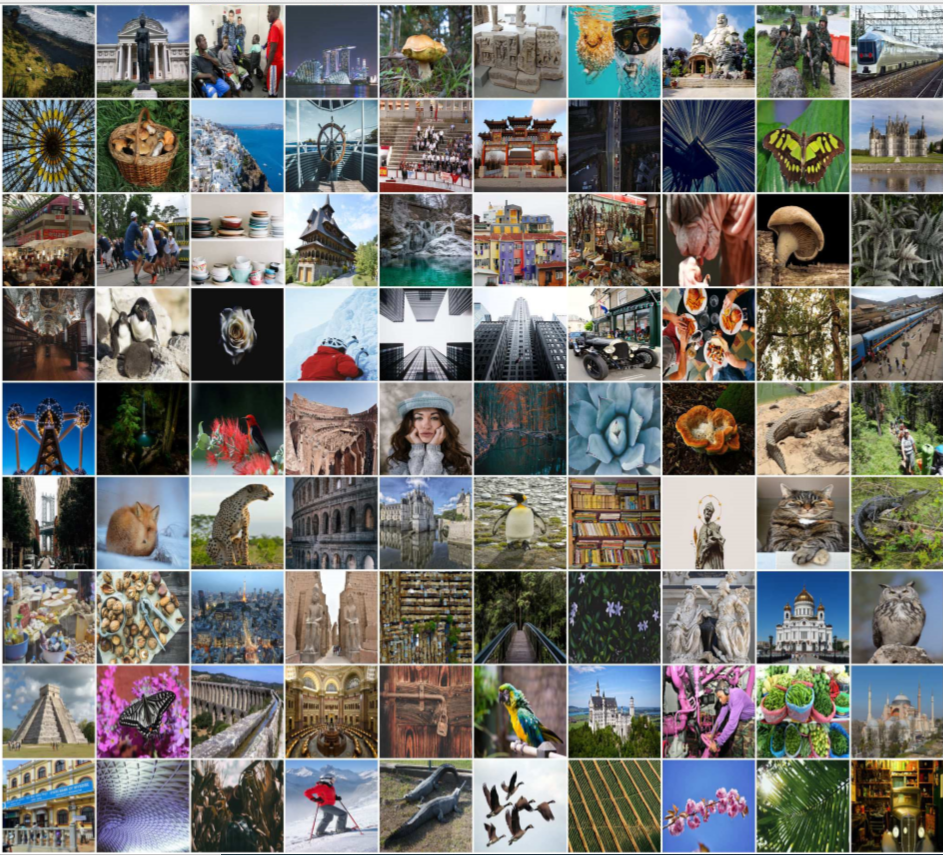
\includegraphics[width=0.85\textwidth]{div2k.png}
\caption{DIV2K validation set examples.
}
\label{fig:div2k}
\end{figure}
\end{center}

In our super resolution applications we used as training set the images provided by the DIV2K (\emph{DIVerse 2K resolution high quality images}) dataset~\cite{Agustsson_2017_CVPR_Workshops}.
This dataset was appositely created for the 2017 NTIRE challenge (\emph{New Trends in Image Restoration and Enhancement}).
The NTIRE challenge is an international competition which aims to monitoring the state-of-art in digital image processing and image analysis and it takes place at the CVPR (\emph{Computer Vision and Pattern Recognition}) conference every year.
One of the most important monitored task is the super resolution research progress.
Thus, every year, many research groups propose new super resolution models, mostly based on neural network models, to improve the state-of-art results on this research field.
The challenge is won by the model which performs the higher PSNR value over a validation set extracted on the DIV2K dataset.
For these reason the DIV2K dataset is considered as a standard for super resolution applications.

The dataset contains 800 high-resolution images as training set and their corresponding low-resolution ones, obtained by different down-sampling methods and different scale factors (2, 3, and 4).
A second set of 100 high-resolution images makes the test set on which the model can evaluate its accuracy: also this second set of images have their low-resolution counterpart.
Finally, a third group of 100 images constitutes the validation set, i.e they are blinded images without their corresponding high resolution counterpart, and they are used to evaluate the results of the models in race.

All the 1000 images are 2K resolution, i.e width and height dimensions must have at least 2K pixels.
The images are collected paying particular attention to the quality, diversity of sources (web sites and cameras) and contents.
The DIV2K images, in fact, collect a large diversity of contents, ranging from people, handmade objects and environments (cities, villages) to natural sceneries (including underwater and dim light conditions) and flora and fauna.
In each image we can find more or less complex shapes, geometries and also some words.
We would stress that no one bio-medical image is contented in the dataset since it is very difficult obtain high quality images of this kind (let alone the problems about copyrights and releases).

In our SR applications we used pre-trained\footnote{
  The developed models were not re-trained due to limited time and low computational architectures available.
} neural network models on the DIV2K and we tested their performances over NMR (Nuclear Magnetic Resonance) images.
The models have never seen this kind of images but during the training they learned a large quantity of shapes that can be \quotes{found} also in bio-medical images.
The bio-medical images were provided by the collaboration with the MRPM group of the Physics Department of the University of Bologna and the Bellaria hospital of Bologna.
We thank the volunteers who perform the NMR acquisitions and shared their data.


\end{document}


\documentclass{standalone}

\begin{document}

\section[Segmentation]{Image Segmentation}\label{segmentation:unet}

\begin{center}
\begin{figure}[htbp]
\centering
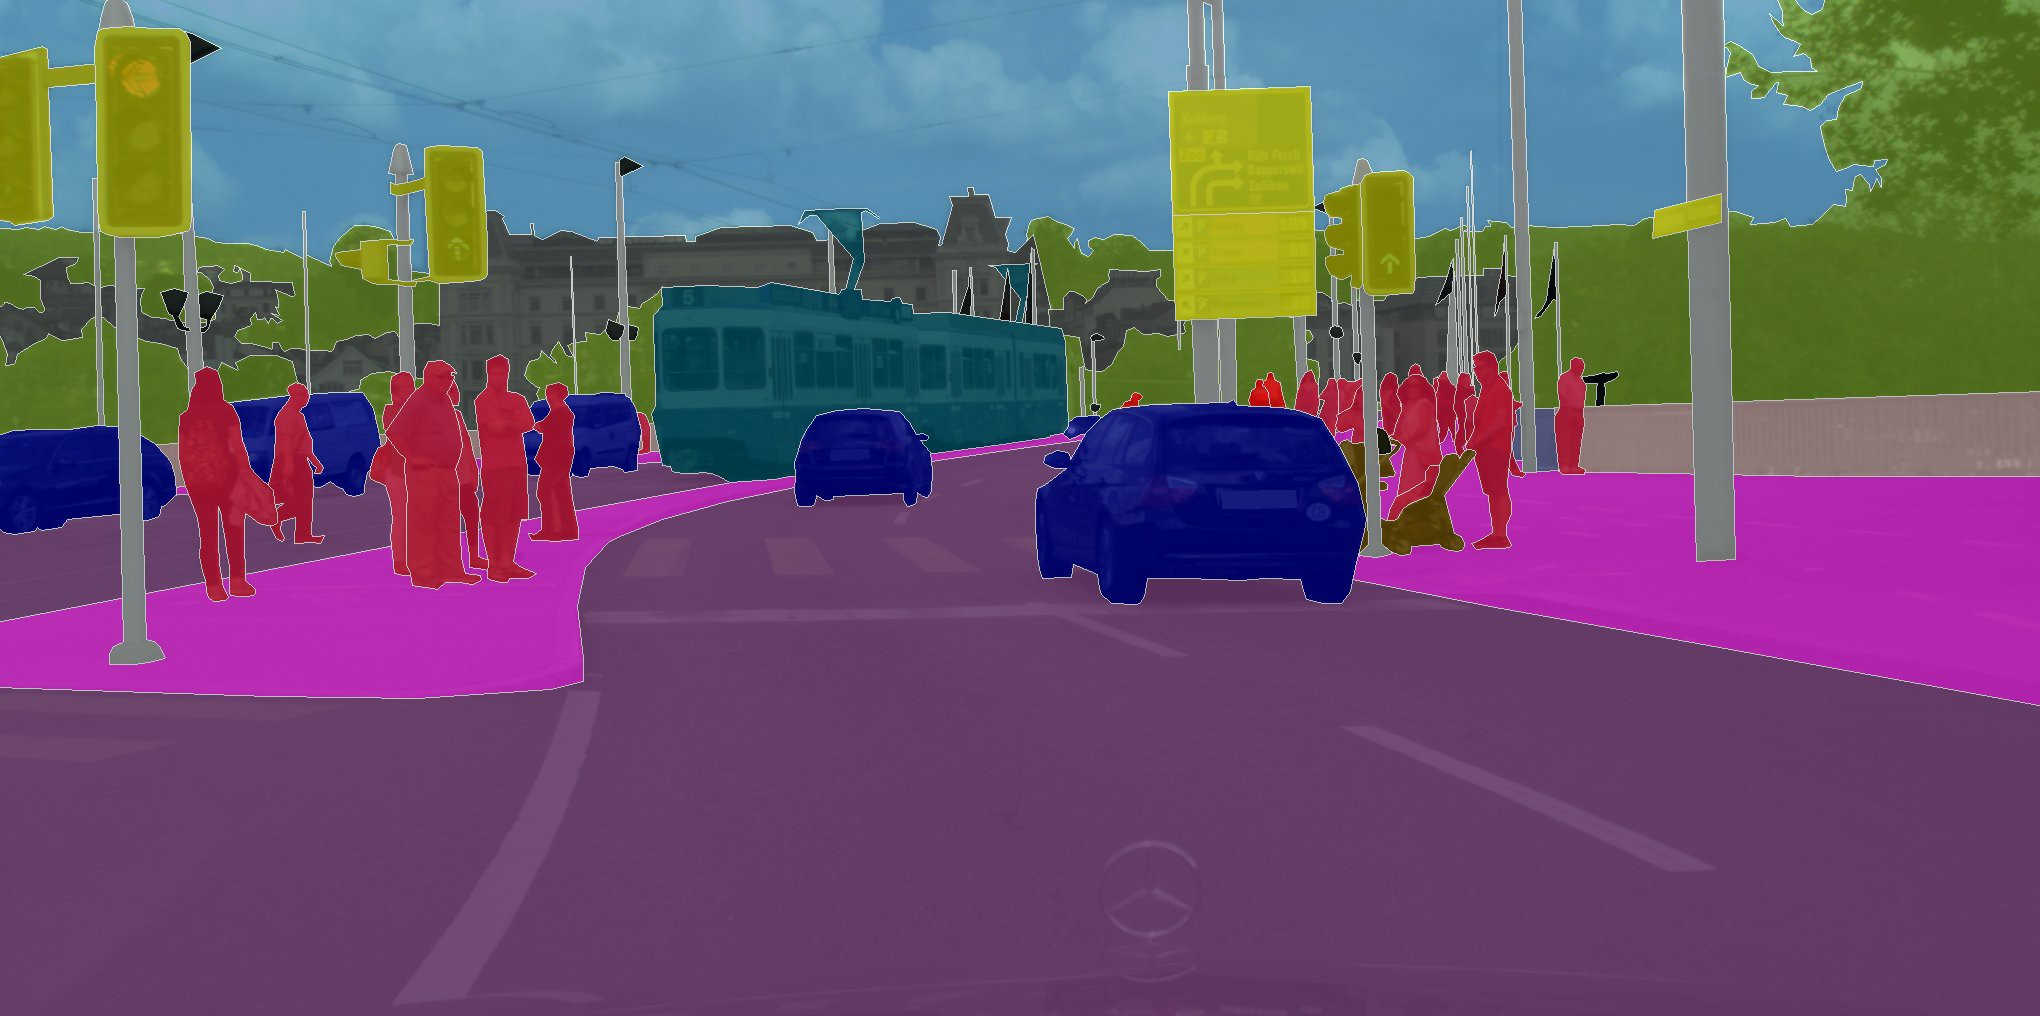
\includegraphics[width=0.85\textwidth]{segmentation.jpg}
\label{fig:segmentation}
\end{figure}
\end{center}

In the previous section we have discussed about the object classification and object detection problems (ref.~\ref{obj_detection:obj}).
Now we want to go deeper on this topic and extract the exact pixels which belong to an object into a given image.
This kind of problem is called Image Segmentation, i.e give a label to each pixel of the input image.

Image segmentation is a typical task in many research fields and could be used for different purposes.
information about pixel-wise position of objects inside an image could be used for extract object shapes from the image or to simplify and/or change the representation of an image into something more meaningful and easier to understand.
This is an hot topic especially for self-driving car applications in which we have to find the exact shapes of object to better estimate their perspective position.
Moreover, all these applications require fast algorithm as much as possible closed to real-time.

This kind of task can be performed using a pipeline of image processing functions or by training a neural network model.
In the first case we have to stack a series of function to process the input image: it has to filters and extracts the useful information about the searched object but most of all it has to be as most general as possible to face on the common heterogeneity of samples.
In the second case we leave to the neural network model parameters the searching of optimal combination of function but we have to provide a supervised input pattern, i.e a combination of input and annotated pixel-wise mask of each image.
The image annotation is one of the most hardest and boring step of image segmentation and for these reasons is very hard to find public dataset usable.

In this chapter we introduce a particular neural network model commonly used in image segmentation problems and we will describe its characteristics and performances.
We applied this model to a novel dataset of CT images.
The dataset annotation was performed by a custom semi-supervised pipeline of image processing and the neural network model was trained and tested on this dataset.
The original data are taken from \href{}{here} and the corresponding annotations are released on \href{}{here}.

\end{document}


\documentclass{standalone}

\begin{document}

\section[rFBP]{Replicated Focusing Belief Propagation}\label{rfbp:rfbp}

Up now we have implicitly talked about Neural Network models based on the standard updating rule of back-propagation.
Other learning rule for weight updates were proposed and the choice of the best one it is still an open-problem.
The final purpose is to obtain a feasible learning rule ables to model the biological learning of the human brain.

The learning problem could be faced through statistical mechanic models joined with the so-called Large Deviation Theory.
In general, the learning problem can be split in two sub-parts: the classification problem and the generalization one.
The first aims to completely store a pattern sample, i.e a prior known ensemble of input-output associations (\emph{perfect learning}).
The second one corresponds to compute a discriminant function based on a set of features of the input which guarantees a unique association of a pattern.

From a statistical point-of-view many Neural Network models have been proposed and the most promising seems to be spin-glass models based.
Starting from a balanced distribution of the system, generally based on Boltzmann distribution, and under proper conditions, we can prove that the classification problem becomes a NP-complete computational problem.
A wide range of heuristic solutions to that type of problems were proposed.

In this section we show one of these algorithms developed by Zecchina et al.~\cite{BaldassiE7655} and called \emph{Replicated Focusing Belief Propagation} (rFBP).
The theoretical background of the algorithm is beyond the scope of this thesis so we focus on its numerical implementation and optimization.

Moreover, despite their proved theoretical efficiency, the applications on real data are still few.
Thus, we show the application of the optimized version of the rFBP algorithm on a Genome Wide Association (GWA) dataset provided by the European \href{https://www.compare-europe.eu/}{COMPARE project}.
This work was also presented on the 2019 CCS-Italy (Conference of Complex System)~\cite{DallOlioCCS19}.

\end{document}

\documentclass{standalone}

\begin{document}


\subsection[Algorithm Optimization]{Algorithm Optimization}\label{rfbp:rFBP}

The rFBP algorithm is a learning algorithm developed to justify the learning process of a binary neural network framework.
The model is based on a spin-glass distribution of neurons put on a fully connected neural network architecture.
In this way each neuron is identified by a spin and so only binary weights (-1 and 1) can be assumed by each entry.
The learning rule which controls the weight updates is given by the Belief Propagation method.

A first implementation of the algorithm was proposed in the original paper~\cite{BaldassiE7655} jointly with an open-source Github repository.
The original version of the code was written in Julia language and despite it is a quite efficient implementation the Julia programming language stays on difficult and far from many users.
To broaden the scope and use of the method, a C++ implementation was developed with a joint \emph{Cython} wrap for Python users.
The C++ language guarantees better computational performances against the Julia implementation and the Python version enlarge its usability.
This implementation is optimized for parallel computing and is endowed with a custom C++ library called \emph{Scorer} (see Appendix D for further details), which is able to compute a large number of statistical measurements based on a hierarchical graph scheme.
With this optimized implementation we try to encourage researchers to approach these alternative algorithms and to use them more frequently on real context.

As the Julia implementation also the C++ one provides the entire rFBP framework in a single library callable via a command line interface.
The library widely uses template syntaxes to perform dynamic specialization of the methods between two magnetization versions of the algorithm.
The main object categories needed by the algorithm are wrapped in handy C++ objects easy to use also from the Python interface.
A further optimization is given by the reduction of the number of available functions: in the original implementation a large amount of small functions are used to perform a single complex computation step, enlarging the amount of call stack; in the C++ implementation the main functions are re-written with the minimizing the call stack to ease the vectorization of the code.

The full rFBP library is released under MIT license and it is open-source on Github~\cite{ReplicatedFocusingBeliefPropagation}.
The on-line repository provides also a full list of installation instructions which could be performed via \emph{CMake} or \emph{Makefile}.
The continuous integration of the project is guaranteed in every operative system using \emph{Travis CI} and \emph{Appveyor CI} which test more than 15 different C++ compilers and environments.

The Python wrap guarantees also a good integration with the other common Machine Learning tools provided by \emph{scikit-learn} Python package; in this way we can use the rFBP algorithm as equivalent alternative also in other pipelines.
Like other Machine Learning algorithm also the rFBP one depends on many parameters, i.e its hyper-parameters, which has to be tuned according to the given problem.
The Python wrap of the library was written according to \emph{scikit-optimize} Python package to allow an easy hyper-parameters optimization using the already implemented classical methods.


\begin{figure}[htbp]
\centering
\def\svgwidth{0.85\textwidth}
\input{./img/rfbp_magp_timing.pdf_tex}
\caption{Comparison of time performances between the original Julia implementation and our Cython one of the rFBP algorithm varying the input dimension sizes (number of samples, $M$, and number of variables, $N$).
For each input configuration 100 runs of both algorithm were performed and the results were normalized by the Julia implementation.
In these cases we fixed the magnetization to \textbf{MagP64}.
}
\label{fig:rfbp_magp}
\end{figure}

\begin{figure}[htbp]
\centering
\def\svgwidth{0.85\textwidth}
\input{./img/rfbp_magt_timing.pdf_tex}
\caption{Comparison of time performances between the original Julia implementation and our Cython one of the rFBP algorithm varying the input dimension sizes (number of samples, $M$, and number of variables, $N$).
For each input configuration 100 runs of both algorithm were performed and the results were normalized by the Julia implementation.
In these cases we fixed the magnetization to \textbf{MagT64}.
}
\label{fig:rfbp_magt}
\end{figure}
%30 (N,M) con N in 1001-5001 con 1000, M=101-351 con 50 ognuna 100 magT

We firstly test the computational efficiency of our implementation against the original Julia one.
The tests were performed comparing our \emph{Cython} version of the code (and thus with a slight overhead given by the Python interpreter) and the Julia implementation as reference.
Varying the dimension sizes (number of samples, $M$, and number of variables, $N$) we tested the time efficiency over 100 runs of both the algorithms.
We divided our simulation according to the two possible type of magnetizations (MagP64 and MagT64 as described by the original implementation available \href{https://github.com/carlobaldassi/BinaryCommitteeMachineFBP.jl}{here}) and the obtained results are shown in Fig.~\ref{fig:rfbp_magp}~\ref{fig:rfbp_magt}, respectively.

As can be seen by the two simulations our implementation always overcome the time performances of the original one, taken as reference in the plot.
However, we can not guarantee a perfect parallel execution of our version: also with multi-threading support the scalability of our implementation does not follow a linear trend with the number of available cores.
In our simulation, in fact, we used 32 cores against the single thread execution of the Julia implementation but we gained only a 4x and 2x of speedup for MagT64 and MagP64, respectively.
The network training is a sequential process by definition and thus it is hard to obtain a relevant speedup using a parallel implementation.
In this case it is probably jointed to a not perfect parallelization strategy chosen which bring to a not efficient scalability of our algorithm version.
However, the many improvements performed to the code allow us to use this algorithm with bigger dataset sizes.

\end{document}

\documentclass{standalone}

\begin{document}


\subsection[Compare dataset]{SNP classification}\label{rfbp:snp}

The few available applications of the rFBP algorithm to real data are amenable to two aspects: I) learning technique; II) algorithm implementation.
The first one is related to the intrinsic definition of the algorithm which is designed to reach a complete memorization of the training dataset; in the other Machine Learning processes we normally want to avoid this kind of results since it could bring to \emph{over-fitting} problems.
The second one is given by the binary values involved in each step of the algorithm which intrinsically limit the possible applications\footnote{
  The Neural Network weights can assume only binary values since they model up/down spins.
  Moreover also the input is required to be a spin configuration and thus binary.
  The common Machine Learning problems involve floating-point values as input pattern.
}.


Classification problems which involved only binary quantities are quite small but the GWA is one of them.
In the GWA we have a series of genome data belonging to different classes as input.
A genome is the ensemble of genes of an organism and each gene is identified by a series of nucleotides with 4 possible values (G, guanine; C, cytosine; A, adenine; T, thymine).
The comparison between a reference (healthy) genome and an infected one highlights the biological mutation related to the understudy disease.
This mutation are the so-called SNPs (Single Nucleotide Polymorphisms).
So we can identify a genome as a sequence of its mutation in relation to a reference genome, i.e a sequence of two possible values given by the on/off of the mutation in each nucleotide.

The COMPARE project aims to develop new methods to avoid the genetic disease transmission.
In this project plays a crucial role the \emph{Source Attribution}, i.e the classification of a given disease based on the list of its mutation.

We tested the rfBP on $210$ Salmonella enterica genome sequences, $4857450\,bp$ (base pairs) long, living inside animals.
Our early goal was to discriminate those bacteria living in pigs (159 samples) with respect to all the others animals (51 samples).

First of all we filter our data removing from each genome a base if it is not mutated in each sample.
In this way we reduce the number of bases to $8189\,bp$.
A graphical representation of these samples is given in Fig.~\ref{fig:SNPsAle}.
The dataset was divided in training and test sets using a stratified cross-validation procedure to guarantee a proportional subdivision of the samples into the two classes.
The algorithm hyper-parameters was tuned on the training set based on the performances obtained using a internal stratified 10-fold cross-validation: in each fold the training was performed by a given sequence of hyper-parameters and the performances evaluated on the corresponding test set; the hyper-parameters configuration which obtains the best performances on the full training set was chosen as best configuration.
The performances evaluation was performed using the custom \emph{Scorer} library.
Considering the unbalanced sample quantities the Matthews Correlation Coefficient (MCC) is chosen as good scorer indicator for the evaluation.

With the tuned hyper-parameters we performed the training of rFBP algorithm on different percentage of the training set: $25\%$, $45\%$, $65\%$ and $85\%$.
In the same way we train also a list of the most common Machine Learning classifiers: single perceptron with floating-point weights (Perc); standard Neural Network with gradient descent as updating rule (MLP); support vector machine with linear kernel (lSVM); support vector machine with radial kernel (rSVM); linear discriminant analysis (LDA); decision tree (DT); random forest (RF); k-nearest neighbors with 2-clusters (kNN); Guassian process (GP); diag-quadratic discriminant analysis (GNB); Bernoulli naive bayes (BNB); AdaBoost (AdaB).
For each training percentage we perform the optimization of the hyper-parameters of each classifier with the same number of optimization steps.
In Fig.~\ref{fig:confronto_bestclassificatoriACC, fig:confronto_best_classificatoriMCC} the accuracies and MCC results are shown, respectively.

From this analysis we can conclude that the rFBP algorithm shows comparable performances with the other classifiers.
These performances globally grow with the training set size but only the rFBP is able to reach a \quotes{perfect learning} configuration, i.e accuracy of 100\% and MCC=1.
We have also noticed that the rFBP classifier and the GNB are the only two algorithms which qualitatively does not show performances saturation on their training.

A second analysis was performed on the data distribution using a multiple $\chi^2$-test.
Starting from the whole set of genomes we can compute the contingency-matrix of the two classes\footnote{
  The contingency-matrix displays the (multivariate) frequency distribution of the variables.
  Each row will count the number of hosts with/without the SNPs.
  Each column will identify a class.
}.
The $\chi^2$-test was performed on the full set of $8189\,bp$ and so the extracted \emph{p-values} were corrected according multiple-tests.
Using the \v{S}id\'ak~\cite{Sidak1967} correction method and by the definition of significant threshold of $0.05$ we found $1103$ significant bases.
An analogous $\chi^2$-test was performed on the rFBP weights to identify a putative

% MISS

\end{document}

\documentclass{standalone}

\begin{document}

\subsection[Results]{Results}\label{rfbp:snp_result}

\begin{figure}[htbp]
\centering
\def\svgwidth{\textwidth}
\input{./img/Ale_ACC_confrontoNicoPhD.pdf_tex}
\caption{Accuracy score obtained on the validation set varying the training set size.
We compared the trends of the whole set of classification algorithms used.
}
\label{fig:confronto_bestclassificatoriACC}
\end{figure}


\begin{figure}[htbp]
\centering
\def\svgwidth{\textwidth}
\input{./img/Ale_MCC_confrontoNicoPhD.pdf_tex}
\caption{Matthews Correlation Coefficient (MCC) score obtained on the validation set varying the training set size.
We compared the trends of the whole set of classification algorithms used.
}
\label{fig:confronto_bestclassificatoriMCC}
\end{figure}

With the tuned hyper-parameters we performed the training of rFBP algorithm on different percentages of the training set: $25\%$, $45\%$, $65\%$ and $85\%$.
In the same way we trained also a list of the most common Machine Learning classifiers: simple Perceptron with floating-point weights (Perc); standard Neural Network with gradient descent as updating rule (MLP); support vector machine with linear kernel (lSVM); support vector machine with radial kernel (rSVM); linear discriminant analysis (LDA); decision tree (DT); random forest (RF); k-nearest neighbors with 2-clusters (kNN); Guassian process (GP); diag-quadratic discriminant analysis (GNB); Bernoulli naive bayes (BNB); AdaBoost (AdaB).
For each training percentage we performed the optimization of the hyper-parameters of each classifier with the same number of optimization steps.
In Fig.~\ref{fig:confronto_bestclassificatoriACC}~\ref{fig:confronto_bestclassificatoriMCC} the accuracies and MCC results are shown, respectively.

From this analysis we can conclude that the rFBP algorithm shows comparable performances with the other classifiers.
These performances globally grow with the training set size, but only the rFBP was able to reach a \quotes{perfect learning} configuration, i.e accuracy of 100\% and MCC=1.
We have also noticed that the rFBP classifier and the GNB were the only two algorithms which qualitatively does not show performance saturation on their training.

A second analysis was performed on the data distribution using a multiple $\chi^2$-test.
Starting from the whole set of genomes we can compute the contingency-matrix of the two classes\footnote{
  The contingency-matrix displays the (multivariate) frequency distribution of variables.
  Each row counts the number of hosts with/without the SNPs.
  Each column identifies a class.
}.
The $\chi^2$-test was performed on the full set of $8189\,bp$ and so the extracted \emph{p-values} were corrected according multiple-tests.
Using the \v{S}id\'ak~\cite{Sidak1967} correction method and by the definition of significant threshold of $0.05$ we found $1103$ significant bases.
An analogous $\chi^2$-test was performed on the rFBP weights to identify a putative correlation between a set of weights and mutated bases.
This second $\chi^2$-test was performed only on the simulation which involved the 85\% of data as training set because it was the case in which the rFBP algorithm shows the better performances than the other classifiers.
We firstly defined a base as significant if its corresponding p-value was less or equal than 0.05: in this way we could associate to each base a numerical weight of 0 if it was not significant an $+1$ or $-1$ if it was, where $+1$ identified the pig class and $-1$ the other one.
The set of weights defined following these instruction could be associated to the \quotes{ideal set}.
In this way we could ensure that if the corresponding rFBP weights were equal to $+1$ in all the significant positions (and thus in all the significant bases) for the pig class, the model output would be $+1$ and $-1$ in the opposite case.
This mechanism follows the Simple Perceptron algorithm scheme (ref. \ref{NN:perceptron}) in which each weight is associated to a given entry of the input samples.
The rFBP algorithm follows the same rules with an activation function given by the Heaviside $\Theta$ and it changes only the updating rule.
Moreover, following this method we could ensure that only the $1103$ significant bases extracted were associated to a not null weight.

We took into account the 10 weights set extracted by the 10-Fold cross validation performed to extract the previous results.
From these 10 sets we extracted the representative one using a simple average of their values: each weight entry was computed as the mean of the 10 weight realizations.
In this way each weight entry was converted to a floating point number and we can easily extract the set of weights perfectly equal to $\pm1$.
From our analyses $5201$ weights were consistently equal to $\pm1$ in all the simulations, i.e the algorithm assigned to $5201$ weights always the same value.
In this way we could consider these weight entries as the significant positions identified by the rFBP algorithm.

These rFBP significant weight set could be compared to the $\chi^2$ ideal set.
From this comparison we noticed a good agreement between the two sets: the major part of the significant bases for the $\chi^2$ multiple test could be found also in the significant weights identified by the 10 realizations of the rFBP algorithm.
In particular, we found that $838/841$ bases were significant for both the methods.
The rFBP algorithm correctly identified $838/848$ significant bases related to the $-1$ class and only $3/255$ bases related to the $+1$ class.

In conclusion, we could prove that the rFBP algorithm is able to identify the major part of the significant polymorphisms in the training set.
However, the use of the only training set to extract the significant weights certainly penalized the rFBP algorithm and a second simulation (without prediction purposes) was performed considering the full set of data, i.e 10 realizations without cross-validation.
In this second case the rFBP significant weights correctly identified $702/1103$ where $696/848$ were related to the $-1$ class and $6/255$ to the $+1$ class.
In both cases we could conclude that the dataset did not contain enough information for the $+1$ class identification for the rFBP algorithm.

Following the above results, a final training was performed using only the significant bases identified by the rFBP algorithm and only the significant bases extracted by the $\chi^2$ multiple test, using the full set of available classifiers.
We noticed how the performances of all the classifiers are significantly better using the bases extracted by the rFBP algorithm (always over the 87\% of accuracy) than the results obtained considering the $\chi^2$ significant bases (only few classifier were able to obtain more than 85\% of accuracy).

We conclude that our results highlight the efficiency of the rFBP algorithm for genome analyses and SNPs classification problems.
Moreover we could propose also the rFBP algorithm as a valid feature selection alternative to classical statistical tests.
These results also encourage us to further investigate about the biological meaning of the significant bases identified.

\end{document}


\end{document}

% Description of the modern deep neural networks with potential applications
% Neural Network laboratory developed in pure numpy. Study of the neural network functionality and testing of the code against tensorflow
% rFBP library to optimize the Julia code with reference to the Scorer library and application to COMPARE data (Daniele Thesis)
% Neural Network library for parallel computing developed in C++ with python wrap. Description of the algorithms and strategies chosen in the library development.
% Introduction on the image classification and detection with Yolo architecture. Implementation in Byron with description of performances against darknet (original implementation). Focus on performances (time, memory, cpu).
% Introduction on Super Resolution problem with focus on state-of-art neural network architecture. Description of the Byron implementation and application on NMR data with the most common measurements. Super-resolution allows better detection!
% Introduction on Image Segmentation problem and application of Unet (Byron implementation) on femur images (TODO)


%% Chapter 3 - CHIMeRA project

\documentclass{standalone}

\begin{document}


\documentclass{standalone}

\begin{document}

\chapter[Big Data]{Biological Big Data - CHIMeRA project}\label{chapter3:bigdata}

\begin{center}
\begin{figure}[htbp]
\centering
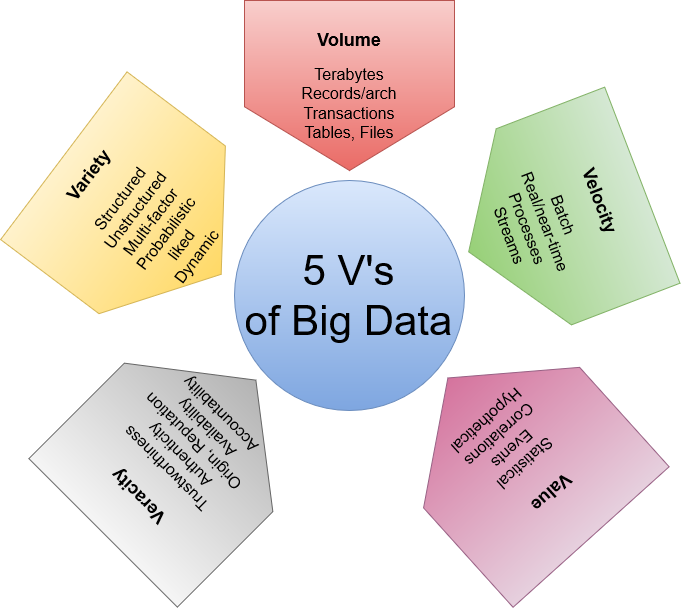
\includegraphics[width=\textwidth]{5v.png}
\caption{Big Data 5 V's}
\label{fig:5v}
\end{figure}
\end{center}

Every second a large quantity of data are produced and shared through Internet and Web-pages.
Data are collected by social networks, messages, video streaming and images.
Everyone, in fact, can easily create new data sources and share or put them in Internet pages.
The growth of this data is not limited to multimedia data but it involves many different fields.
This is one of the most important feature of the contemporary time, the so-called Big Data era: this huge volume of data has created a new field in data processing which is called Big Data Analytics that nowadays positioned among top ten strategic technologies (Gartner Research, 2012).

It is still difficult to provide a definition of what exactly are the Big Data and we can find many slight different nomenclatures and categories which aim to formulate it.
Moreover, Big Data does not define a particular data type but more than we normally think sources can be labeled as it.
The \emph{International Journal of Computer Applications} defined them as \quotes{$[\cdots]$ a collection of large and complex datasets that cannot be processed and analyzed using traditional computing techniques. It is not a single technique or a tool, rather it involves many areas of business and technology}.
This definition certainly involves many aspects of Big Data processing but it does not provide any definition about their nature.
Moreover, it is easy to identify them as \quotes{big} and thus difficult to analyze, but they are all around us every day and just using the Internet connection every smart-phone or laptop can extract and visualize our web queries so could be not properly correct to define them in this way.
However it is certainly sure that the standard computing techniques have to be reviewed to face on this vast amount of data and a even more important attention has to be payed on the algorithm implementations.

While a global definition of them is evidently difficult we can however describe them using some of their \quotes{essential} features.
One of the most common and used set of labels is given by the so called 5 V's of Big Data: volume, velocity, variety, veracity and value.
Despite the first twos are quite obvious (the Big Data are certainly \emph{big} in volume and they are produced very \emph{fast}), the remaining three need a particular attention.
Moreover, we have already treated problems about the volume of data (ref. Chapter\ref{chapter1:featsel}) and the need of very fast processing and algorithm optimizations (ref. Chapter\ref{chapter2:neural}).
Now in this chapter we want to focus on the remaining three characteristics of Big Data Analytics.

As pre-announced there many different sources able to provide data and this feature describes the extreme heterogeneity and variety of them.
We can however broadly classify this variety into three global classes: \emph{structured data}, \emph{semi-structured data} and \emph{unstructured}.
A dataset is \emph{structured} if we can easily manage the informations in it or, in other words, if it is described using the standard formats of data and thus can it can be \quotes{quearable}.
On the other side we have the completely \emph{unstructured} dataset in which the data are disorganized and we need one or multiple pre-processing steps before use them or we have to develop different techniques to handle them.
The intermediate step is given by the \emph{semi-structured} data in which only a part of them could be handle with standard techniques or can be easily brought to their structured version.
The data organization has been a crucial task on this work of thesis and we will return on this topic in the next sections.

The fourth essential characteristic of Big Data is the \emph{veracity} of them due to data inconsistency and incompleteness.
The data are shared very fast using Internet and there could be found some ambiguities and/or deceptions between different data sources.
If we want to merge and aggregate different kind of informations we have also to face on this kind of problems.
The final task of every Big Data Analytic application is, in fact, to process these large quantities of data and obtain a unique answer which can not vary in relation to the portion of data or dataset used.

The last and probably most important feature is certainly their \emph{value}: it is certainly good to have access to large amount of data but unless we can turn them into value they are useless.
In this vast amount of data only a small part of them can be considered as informative and it is always harder to extract this core of informations from them.
Moreover, we have to take into account also the difficulties about the management of these data and their more or less complex structure.
However, also in this case, it is hard to generalize this property on all the amount of data contained in Internet: every day we see a large quantity of useless information on the web and it is hard to figure out that some of them can be useful for research applications.
A key role is played by the \emph{questions} which we ask: for every data source there is always an appropriated question which can be answer using it and vice versa.
In this way also the seemingly useless datasets can acquire importance for an appropriated research project.

In this chapter we will discuss about one of the latest project developed during my PhD and which is still in work in progress: the CHIMera (\emph{Complex Human Interactions in MEdical Records and Atlases}) project.
The project is founded on Big Data applications and it is accidentally born as separated branch of the INFN FiloBlu project (ref. next sections and Appendix E for further informations about the project) which financed my last PhD year.
CHIMeRA aims to create a unified database of bio-medical records using Natural Language processing techniques.
The final purpose is to merge multiple data sources available on-line into a single network structure which highlights the relevant interactions between bio-medical informations, i.e starting from diseases to the biological agents involved into their causes and consequences.
The realization of the first version of CHIMeRA required a lot of time and the development of novel pipelines of data processing.
The project does not still achieve its conclusions but in this chapter we will cross through the main key points which allowed its construction.

%talk about data structured and unstructured
%Many public datasets available.
%Description of the database used in chimera.
%Problems about the intersections and partial informations (single db).


\end{document}
 % Neural Network introduction

\documentclass{standalone}

\begin{document}

\section[CHIMeRA]{The CHIMeRA project}\label{chimera:chimera}

The increasing availability of large-scale biomedical literature under the form of public on-line databases, has opened the door to a whole new understanding of multi-level associations between genomics, protein interactions and metabolic pathways for human diseases via network approaches.
Many structures and resources aiming at such type of analyses have been built, with the purpose of disentangling the complex relationships between various aspects of the human system relating to diseases~\cite{SymtomsNet, HumanPhenotype}.

%What is CHIMeRA project and which is its potentiality.
%Description of the database created and of the query implemented to obtain the results %TODO: better query


\end{document}

\documentclass{standalone}

\begin{document}

\section[CHIMeRA query]{CHIMeRA query}\label{query:query}

%Some query examples like leukemia subnetwork and PRNP subnetwork.
%Description of the information extracted by these subnetworks. % TODO

\end{document}

\documentclass{standalone}

\begin{document}

\section[Web Scraping]{Data extraction - Web scraping}\label{scraping:scraping}

%Description of the web scraping techinques used to obtain the "no-public" datasets.
%Reference to the github project.


\end{document}

\end{document}

% Many public datasets available. Description of the database used in chimera
% Description of the web scraping techinques used to obtain the "no-public" datasets. Reference to the github project
% What is CHIMeRA project and which potentiality it has. Description of the database created and of the query implemented to obtain the results (TODO: better query)
% Some query examples like leukemia subnetwork and PRNP subnetwork. Description of the information extracted by these subnetworks


%% Chapter 4 - cardiological data

% \input{./tex/Chapter4/AppitechData.tex}
% % Description of the pulsoximmetry and of the cardiological data analyzed

% \input{./tex/Chapter4/CardioFeature.tex}
% % Description of the features extracted on the cardiological dataset

% \input{./tex/Chapter4/AgePrediction.tex}
% % Pipeline of the feature selection with age prediction obtained on cardio data

%% Conclusion

\documentclass{standalone}

\begin{document}

\chapter*{Conclusions}\label{conclusions}\addcontentsline{toc}{chapter}{Conclusions}
\markboth{Conclusions}{Conclusions}

We have concluded our discussion about the applications of Big Data Analytic algorithms to Biomedical data.
In this work we have touched several and different topics related to this theme.

In the first chapter we have focused on the difficulties about information extraction, analyzing high-throughput datasets.
The so-called \emph{omics} datasets are becoming a very interesting research field in biology and medicine since, using modern data acquisition techniques, they are capable to give a wide range of useful data for the analysis of multiple diseases.
A crucial role on this topic is given by tumors and, using \emph{omic} data, we can design novel methods to identify the agents responsible for these diseases.
Biomedical Big Data pose new challenges to the scientific research, since we have to convert them into useful information or, in other words, we have to be able to identify their informative cores.
To this purpose we have designed the new \textsf{DNetPRO} algorithm as a novel feature selection method.

We have tried to show all the pros and cons about the proposed algorithm.
Only knowing its limits we could be able to provide a reasonable interpretation about its results and for this reason we firstly tested our method on synthetic data.
The proposed \textsf{DNetPRO} pipeline was tailored on gene expression applications and we have shown its application on real data, comparing its efficiency against other state-of-art models in which it is able to outperform them in the major part of the analyzed cases.
Some these results are already published in international papers or they are in press.
We would remark that \textsf{DNetPRO} could be used also as standalone feature selection algorithm, but, for sake of brevity, we have discussed its application on non-biological data only in the Appendices of this work.

In the second chapter we have moved to numerical applications in the deep learning research field.
We have paid particular attention to the description and optimization of some state-of-art deep learning models.
In this chapter we have also introduced three new custom libraries about this topic, which have been developed with different purposes: the \textsf{NumPyNet} is essentially an educational framework for the development of neural network models, while the \textsf{Byron} library is focused on the numerical performances; the \textsf{rFBP} library was designed for very particular applications and in this work we have just briefly shown one of them.
Starting from the bases of neural network models, we have discussed about different kinds of functions (more or less straightforward) which are commonly involved in the construction of a deep learning neural network architecture.
For each function, we have only summarily described its mathematical background, focusing instead on the critical points related to its algorithmic implementation.

We have used the two developed libraries (\textsf{NumPyNet} and \textsf{Byron}) to highlight possible ways to overcome these numerical issues.
For sake of brevity, it has not been possible to go in deeper details about the numerical improvements performed, but all the developed codes have been shared and they are publicly available on the author's Github page.
The modern scientific research, in fact, is not made only by papers and publications but it is acquiring even more importance the code development and, thus, its public availability.
By sharing our code on the Internet, we want to encourage the research community to take in consideration also our promising results about these topics.
We have touched different state-of-art models and implementations of them along our discussion and in all the analyzed cases our results overcome them with not negligible results.

The results obtained using Super Resolution and Segmentation models are very promising for the analysis of biomedical images.
Moreover, we have shown that deep learning models are capable of a very efficient generalization due to their vast amount of parameters and a well-programmed training section.
In particular, our Super Resolution models were trained on general-purpose (natural) images, but they are, however, able to reconstruct biomedical NMR images better than standard methods.
This, already discussed, result is due to the ability of the model in the identification of analogous textures and patterns between the training and validation images, without need of a tailored retrain.
We have also seen how we can improve object detection efficiency using a pre - Super Resolution - processing: we could not show biomedical results on this topic due to lack of data and privacy reasons, but we have shown how a people-counting problem (Complex System task) is improved by this.

We would remark that our work was focused on the optimization of those codes only for CPU usages and, thus, we can not compare them to the wide world of GPU deep learning models.
We would, however, stress that we have intentionally chosen to focus only on these computational environments, aiming to increase the usage of this kind of models also in research fields which do not need GPUs in their everyday works.
There are, in fact, a lot of scientific applications which are tailored on CPUs architectures and which are pushed out to the deep learning researches, or which do not even try to use deep learning models afraid by their intensive computational demand.
We developed the \textsf{Byron} library to overcome these issues and to highlight how a well-thought-out algorithmic implementation can overcome also the more computational expensive applications.

All the developed algorithms were intensively profiled against other state-of-art implementations and their pros and cons have been examined in order to find the best solution for a given problem.
Code testing has been performed also on different operative systems, since how well an algorithm is made, it is useless if it works only on a well-defined machine.
A continuous integration of our codes has been at the basis of all the proposed libraries, as much as a reliable and user-friendly code documentation.

We have concluded our discussion introducing the \textsf{CHIMeRA} project which, even though the analysis of its results is still in work in progress, gives us multiple points of discussion about Biomedical Big Data.
There is an increasing interest about database harmonization in the last years and its need is given by the growing amount of publicly available data.
The research community is still trying to keep up with the new demand of data analysis and an increasingly important role is played by the development of new computational strategies and techniques.
Many European projects financed by the Horizon 2020 Research and Innovation program are focused on this topic and a particular attention is paid on the health-care research.

The \textsf{CHIMeRA} project could not be compared to such big research programs, but it is driven by the same kind of ideas.
Its final purpose, in fact, is to use the wide range of available information and results, obtained by independent research studies, and combine them into a unique framework of analysis.
Observational databases differ in both purposes and designs: they have been collected for different purposes and the logical organizations as much the medical terminologies can vary from source to source.
A \emph{Common Data model} (CDM) is designed to overcome these issues and to offer a unique solution for the information storage in the same way as our \textsf{CHIMeRA} project merges together information provided by multiple on-line databases.
Unfortunately, the research community is developing a wide range of CDMs and as long as a single solution is not taken as standard, the problem can not be solved.
Also in this case, we have not developed \textsf{CHIMeRA} as putative alternative to this purpose, but it is simply a temporary solution which allows us to perform a panoramic overview of biomedical agents.

We have highlighted multiple possible usages of the developed \textsf{CHIMeRA} network-of-networks structure and we hope it can be useful as an integrative tool also for the biggest projects like the HARMONY one.
In this work we have focused on the key steps which lead us to the ideas behind the \textsf{CHIMeRA} project and, moreover, we have described difficulties and their relative proposed solutions about the creation of a such network-of-networks database.
Despite the work has been intense up to now, the more interesting part from a scientific point-of-view is just began.
The \textsf{CHIMeRA} database is the only \quotes{code} discussed in this work which is not yet publicly available, due to its embryonic stage, but hopefully we can provide its first release as soon as possible.


\end{document}


%% Acknowledgment

\pagenumbering{gobble}% Remove page numbers (and reset to 1)
\documentclass{standalone}

\begin{document}

\chapter*{Acknowledgment}

\end{document}


%% Appendix

\documentclass{standalone}

\begin{document}

\documentclass{standalone}

\begin{document}

\chapter*{Appendix A - Discriminant Analysis}\addcontentsline{toc}{chapter}{Appendix A - Discriminant Analysis}
\markboth{Appendix A}{Discriminant Analysis}

The classification problems aim to associate a set of \emph{pattern} to one or more \emph{classes}.
With a \emph{pattern} we identify a multidimensional array of data labeled by a pre-determined tag.
In this case we talk about \emph{supervised learning}, i.e the full set of data is already annotated and we have prior knowledge about the association between data and classes.

In machine learning a key rule is played by Bayesian methods, i.e methods which use a Bayesian statistical approach to the analysis of data distributions.
It can be proved that, if the underlying distributions are known, i.e a sufficient number of its moments are known with a sufficient precision, the Bayesian approach is the best possible method to face the classification problem (\emph{Bayesian error rate}\cite{Fukunaga:1990:ISP:92131}).

\end{document}

\documentclass{standalone}

\begin{document}


\section*{Mathematical background}\addcontentsline{toc}{section}{Mathematical background}
\markboth{Appendix A}{Mathematical background}

The exact knowledge of prior probabilities and conditional probabilities are generally hard to evaluate thus a parametric approach is often needed.
A parametric approach aim to create reasonable hypothesis about the data distribution and its fundamental parameters (e.g mean, variance, $\cdots$).
In the following discussion, we are going to focus only on normal distributions for mathematical convenience but the results could be easily generalized.

Given the multi-dimensional form of Gauss distribution:

$$
G(\mathbf{x}|\mu, \Sigma) = \frac{1}{(2\pi)^{d/2}\cdot\left|\Sigma\right|^{1/2}}\cdot exp\left[-\frac{1}{2}(\mathbf{x}-\mathbf{\mu})^T\Sigma^{-1}(\mathbf{x}-\mathbf{\mu})\right]
$$
\\
where $\mathbf{x}$ is a $d$-dimensional column vector, $\mathbf{\mu}$ is the mean vector of the distribution, $\Sigma$ is the covariance matrix ($d\times d$) and $|\Sigma|$ and $\Sigma^{-1}$ the determinant and the inverse of $\Sigma$, respectively, we can notice the quadratic dependence of $G$ depends by $\mathbf{x}$,

$$
\Delta^2 = (\mathbf{x}-\mu)^T\Sigma^{-1}(\mathbf{x}-\mu)
$$
\\
where the exponent ($\Delta^2$) is called \emph{Mahalanobis distance} of vector $\mathbf{x}$ from its mean.
This distance can be reduced to the Euclidean one when the covariance matrix is the identity matrix ($\mathbf{I}$).

The covariance matrix is always symmetric and positive semi-definite by definition (useful informations for the next algorithmic strategies) so it is invertible.
If the covariance matrix has only diagonal terms the multidimensional distribution can be expressed as the simple product of $d$ mono-dimensional normal distributions.
In this case the main axes are parallel to the Cartesian axes.

Starting from a multi-variate Gaussian distribution\footnote{
  In Machine Learning it will correspond to the conditional probability density.
}, the Bayesian rule for classification problems can be rewritten as:

$$
g_i(\mathbf{x}) = P(w_i|\mathbf{x}) = \frac{p(\mathbf{x}|w_i)P(w_i)}{p(\mathbf{x})} = \frac{1}{(2\pi)^{d/2}\cdot\left|\Sigma_i\right|^{1/2}}\cdot exp\left[-\frac{1}{2}(\mathbf{x}-\mathbf{\mu_i})^T{\Sigma_i}^{-1}(\mathbf{x}-\mathbf{\mu_i})\right] \frac{P(w_i)}{p(\mathbf{x})}
$$
\\
where, removing constant terms ($\pi$ factors and the absolute probability density $p(\mathbf{x}) = \sum_{i=1}^s p(\mathbf{x}|w_i)\cdot P(w_i)$) and using the monotonicity of the function, we can extract the logarithmic relation:

$$
g_i(\mathbf{x}) = -\frac{1}{2}(\mathbf{x}-\mu_i)^T{\Sigma_i}^{-1}(\mathbf{x}-\mu_i) -\frac{1}{2}\log\left|\Sigma_i\right|+\log P(w_i)
$$
\\
which is called \emph{Quadratic Discriminant function}.

The dependency by the covariance matrix allows 5 different cases:

\begin{itemize}

\item \textbf{$\Sigma_i=\sigma^2I$ - DiagLinear Classifier}

\begin{minipage}{.30\textwidth}
\hspace{-.5cm}
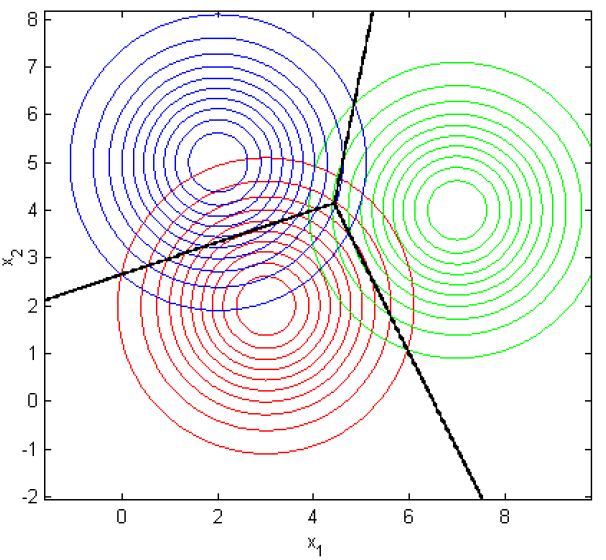
\includegraphics[width=1\textwidth]{case1.png}
\end{minipage}%
\begin{minipage}{.70\textwidth}
This is the case in which features are completely independent, i.e they have equal variances for each class.
This hypothesis allows us to simplify the discriminant function as:
\end{minipage}\\

$$
g_i(\mathbf{x})=-\frac{1}{2\sigma^2}(\mathbf{x^Tx}-2{\mu_i}^T\mathbf{x} + {\mu_i}^T\mu_i) + \log P(w_i)
$$
\\
and removing all the $\mathbf{x^Tx}$ constant terms for each class

$$
g_i(\mathbf{x}) = -\frac{1}{2\sigma^2}(-2{\mu_i}^T\mathbf{x}+{\mu_i}^T\mu_i)+\log P(w_i) = \mathbf{{w_i}^Tx}+\mathbf{w_0}
$$
\\
These simplifications create a linear discriminant function and the separation surfaces between classes are hyper-planes ($g_i(\mathbf{x})=g_j(\mathbf{x})$).

With equal prior probability the function can be rewritten as

$$
g_i(\mathbf{x}) = -\frac{1}{2\sigma^2}(\mathbf{x}-\mu_i)^T(\mathbf{x}-\mu_i)
$$
\\
which is called \emph{nearest mean classifier} and the equal-probability surfaces are hyper-spheres.


\item \textbf{$\Sigma_i = \Sigma$ (diagonal matrix) - Linear Classifier}

\begin{minipage}{.30\textwidth}
\hspace{-.5cm}
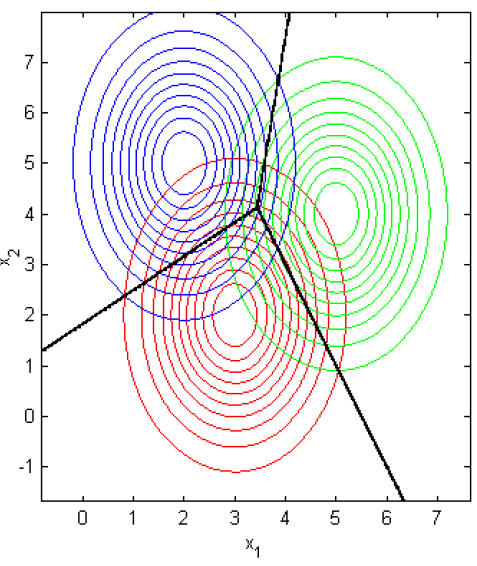
\includegraphics[width=1\textwidth]{case2.png}
\end{minipage}%
\begin{minipage}{.70\textwidth}
In this case the classes have same covariances but each feature has its own different variance.
After the substitution of $\Sigma$ in the equation, we obtain
\end{minipage}\\

$$
g_i(\mathbf{x}) = -\frac{1}{2}\sum_{k=1}^{s}\frac{(\mathbf{x_k}-\mu_{i,k})^2}{{\sigma_k}^2}-\frac{1}{2}\log\prod_{k=1}^{s}{\sigma_k}^2+\log P(w_i)
$$
\\
where we can remove constant $\mathbf{x_k}^2$ terms (equal for each class) and obtain another time a linear discriminant function and discriminant surfaces given by hyper-planes and equal-probability boundaries given by hyper-ellipsoids.
We remark that the only difference from the previous case is the normalization factor of each axis that in this case is given by its variance.


\item \textbf{$\Sigma_i = \Sigma$ (non-diagonal matrix) - Mahalanobis Classifier}

\begin{minipage}{.30\textwidth}
\hspace{-.5cm}
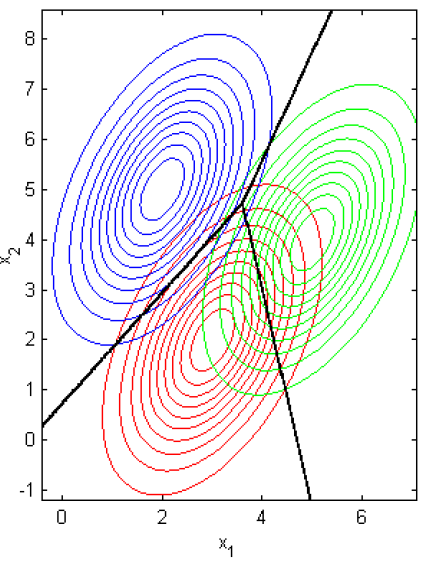
\includegraphics[width=1\textwidth]{case3.png}
\end{minipage}%
\begin{minipage}{.70\textwidth}
In this case we assume that each class has the same covariance matrix but they are non-diagonal ones.
The discriminant function becomes
\end{minipage}\\

$$
g_i(\mathbf{x}) = -\frac{1}{2}(\mathbf{x}-\mu_i)^T{\Sigma}^{-1}(\mathbf{x}-\mu_i) -\frac{1}{2}\log\left|\Sigma\right|+\log P(w_i)
$$
\\
where we can remove the $\log\left|\Sigma\right|$ term because it is constant for all the classes and we can assume equal prior probability.
In this case we obtain

$$
g_i(\mathbf{x}) = -\frac{1}{2}(\mathbf{x}-\mu_i)^T{\Sigma}^{-1}(\mathbf{x}-\mu_i)
$$
\\
where the quadratic term is the above told \emph{Mahalanobis distance}, i.e a normalization of the distance according to the inverse of the covariance matrix.
We can prove that expanding the scalar product and removing the constant $\mathbf{x^T\Sigma^{-1}x}$ term, we still obtain a linear discriminant function with the same properties of the previous case.
In this case the hyper-ellipsoids have axes aligned to the eigenvectors of the $\Sigma$ matrix.


\item \textbf{$\Sigma_i = {\sigma_i}^2I$ - DiagQuadratic Classifier}

\begin{minipage}{.30\textwidth}
\hspace{-.5cm}
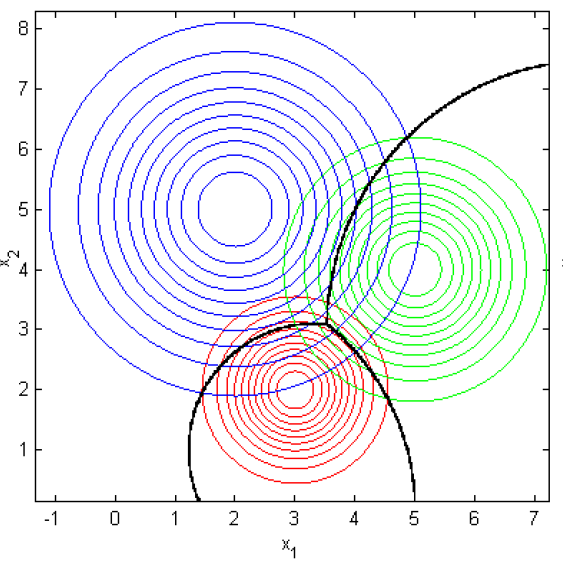
\includegraphics[width=1\textwidth]{case4.png}
\end{minipage}%
\begin{minipage}{.70\textwidth}
In this case we have a different covariance matrix for each class but they are all proportional to the identity matrix, i.e diagonal matrix.
The discriminant function in this case becomes
\end{minipage}\\

$$
g_i(\mathbf{x}) = -\frac{1}{2}(\mathbf{x}-\mu_i)^T{\sigma_i}^{-2}(\mathbf{x}-\mu_i) -\frac{1}{2}s\log\left|{\sigma_i}^2\right|+\log P(w_i)
$$
\\
where this expression can be further reduced obtaining a quadratic discriminant function.
In this case the equal-probability boundaries are hyper-spheres aligned to the feature axes.


\item \textbf{$\Sigma_i \neq\Sigma_j$ (general case) - Quadratic Classifier}

\begin{minipage}{.30\textwidth}
\hspace{-.5cm}
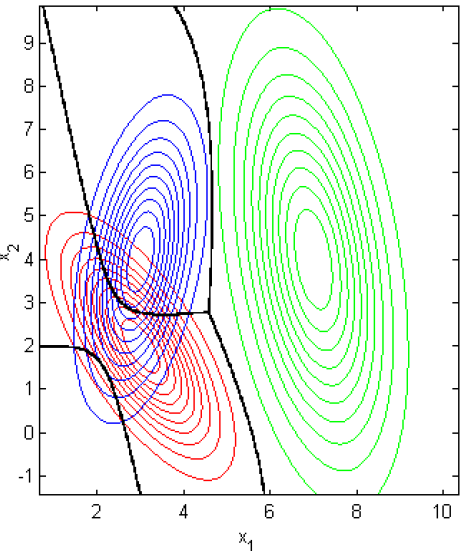
\includegraphics[width=1\textwidth]{case5.png}
\end{minipage}%
\begin{minipage}{.70\textwidth}
Starting from the more general discriminant function we can relabel the variables and highlight its quadratic form as
\end{minipage}\\

$$
g_i(\mathbf{x}) = \mathbf{x^TW_{2,i}x}+\mathbf{w_{1,i}^Tx} + \mathbf{w_{0,i}} \quad \mbox{with}\quad \left\{\begin{array}{l} \mathbf{W_{2,i}}=-\frac{1}{2}{\Sigma_i}^{-1}\\ \mathbf{w_{1,i}}={\Sigma_i}^{-1}\mu_i \\ \mathbf{w_{0,i}}=-\frac{1}{2}{\mu_i}^T{\Sigma_i}^{-1}\mu_i-\frac{1}{2}\log\left|\Sigma_i\right|+\log P(w_i) \\ \end{array}\right.
$$
\\
In this case each class has its own covariance matrix $\Sigma_i$ and the equal-probability boundaries are hyper-ellipsoids oriented to the eigenvectors of the covariance matrix of each class.

\end{itemize}

The Guassian distribution hypothesis of data should be tested before using this classifiers.
It can be evaluated using statistical tests as \href{https://www.jstor.org/stable/2284163?seq=1#page_scan_tab_contents}{\emph{Malkovich-Afifi}} based on \href{https://en.wikipedia.org/wiki/Kolmogorov–Smirnov_test}{\emph{Kolmogorov-Smirnov}} index or using the empirical visualization of the data points.


\end{document}

\documentclass{standalone}

\begin{document}

\section*{Numerical Implementation}\addcontentsline{toc}{section}{Numerical Implementation}
\markboth{Appendix A}{Numerical Implementation}

From a numeric point of view we can exploit each mathematical information and assumption to simplify the computation and improve the numerical stability of our computation.
I would remark that this consideration were taken into account in this work only for the C++ algorithmic implementation since these methods are already implemented in the high-level programming languages as \emph{Python} and \emph{Matlab}\footnote{
  For completeness we have to highlight that for the Matlab case classification functions, i.e \emph{classify}, is already included in the base packages of the software, i.e no external Toolbox are needed, while for the Python case the most common package which implements these techniques are given by the \emph{scikit-learn} library.
  Matlab allows to set the classifier type as input parameter in the function using a simple string which follows the same nomenclature previously proposed.
  Python has a different import for each classifier type: in this case we find correspondence between our nomenclature and the Python one only in \emph{quadratic} and \emph{linear} cases, while the \emph{Mahalanobis} is not considered a putative classifier.
  The \emph{diagquadratic} classifier is called \emph{GaussianNB} (\emph{Naive Bayes Classifier}) instead.
  The last important discrepancy between the two language implementation is in the computation of the variance (and the corresponding covariance matrix): Matlab proposes the variance estimation only in relation to the mean so the normalization coefficient is given by the number of sample except by one ($N-1$), while Python compute the variance with a simple normalization by $N$.
}.

In the previous section we highlight that the covariance matrix is a positive semi-definite and symmetric matrix by definition and this properties allows the matrix inversion.
The computation of the inverse-matrix is a well known complex computation step from a numerical point-of-view and in a general case can be classified as an $O(N^3)$ algorithm.
Moreover the use of a Machine Learning classifier commonly match the use of a cross validation method, i.e multiple subdivision of the dataset in a training and test sets.
This involves the computation of multiple inverse matrix and it could represent the performance bottleneck in many cases (the other computations are quite simple and the algorithm complexity is certainly less than $O(N^3)$).

Using the information about the covariance matrix we can find the best mathematical solution for the inverse matrix computation that in this case is given by the Cholesky decomposition algorithm.
The Cholesky decomposition or Cholesky factorization allows to re-write a positive-definite matrix into the product of two triangular matrix (the first is the conjugate transpose of the second)

$$
\mathbf{A} = \mathbf{LL^T} = \mathbf{U^TU}
$$
\\
The complexity of the algorithm is the same but the inverse estimation is simpler using a triangular matrix and the entire inversion can be performed in-place.
It can also be proved that general inverse matrix algorithms have numerical instability problems compared to the Cholesky decomposition.
In this case the original inverse matrix can be computed by the multiplication of the two inverses as

$$
\mathbf{A^{-1}} = (\mathbf{L^{-1}})^T(\mathbf{L^{-1}}) = (\mathbf{U^{-1}})(\mathbf{U^{-1}})^T
$$
\\
As second bonus, the cross validation methods involve the subdivision of the data in multiple non-independent chunks of the original data.
The extreme case of this algorithm is given by the Leave-One-Out cross validation in which the superposition of the data between folds are $N-1$ (where $N$ is the size of the data).
The statistical influence of the swapped data is quite low and the covariance matrix will be quite similar between one fold to the other (the inverse matrix will be drastically affected from each slight modification of the original matrix instead).
A second step of optimization can be performed computing the original full-covariance matrix of the whole set of data ($O(N^2)$) and at each cross-validation step evaluate the right set of $k$ indexes needed to modify the matrix entrances ($O(N*k)$) that in the Leave-One-Out case are just one.
This second optimization consideration can also be performed in the Diag-Quadratic case substituting the covariance matrix with the simpler variance vector.

% maybe insert some code snippets

Both these two techniques were used in the custom C++ implementation of the Quadratic Discriminant Analysis classifier and in the Diag-Quadratic Discriminant Analysis classifier for the DNetPRO algorithm implementation (see~\ref{dnetpro:DNetPRO}).


\end{document}



\documentclass{standalone}

\begin{document}

\chapter*{Appendix B - Venice Road Network}\addcontentsline{toc}{chapter}{Appendix B - Venice Road Network}
\markboth{Appendix B}{Venice Road Network}

Tourist flows in historical cities are continuously growing in a globalized world and adequate governance processes, politics and tools are necessary in order to reduce impacts on the urban livability and to guarantee the preservation of cultural heritage.
The ICTs offer the possibility of collecting large amount of data that can point out and quantify some statistical and dynamic properties of human mobility emerging from the individual behavior and referring to a whole road network.
In this work we analyze a new dataset that has been collected by the Italian mobile phone company TIM, which contains the GPS positions of a relevant sample of mobile devices when they actively connected to the cell phone network.
Our aim is to propose innovative tools allowing to study properties of pedestrian mobility on the whole road network.
Venice is a paradigmatic example for the impact of tourist flows on the resident life quality and on the preservation of cultural heritage.
The GPS data provide anonymized geo-referenced information on the displacements of the devices.
After a filtering procedure, we develop specific algorithms able to reconstruct the daily mobility paths on the whole Venice road network.
The statistical analysis of the mobility paths suggests the existence of a travel time budget for the mobility and points out the role of the rest times in the empirical relation between the mobility time and the corresponding path length.
We succeed to highlight two connected mobility subnetworks extracted from the whole road network, that are able to explain the majority of the observed mobility.
Our approach shows the existence of characteristic mobility paths in Venice for the tourists and for the residents.
Moreover the data analysis highlights the different mobility features of the considered case studies and it allows to detect the mobility paths associated to different points of interest.
Finally we have disaggregated the Italian and foreigner categories to study their different mobility behaviors.

\end{document}

\documentclass{standalone}

\begin{document}

\section*{The datasets}\addcontentsline{toc}{section}{The datasets}
\markboth{Appendix B}{The datasets}

The dataset used in this study has been provided by the Italian mobile phone company TIM and contains geo-referenced positions of tens of thousands anonymous devices (e.g. mobile phones, tablets, etc. ...), whenever they performed an activity (e.g. a phone call or an Internet access) during eight days from 23/2/2017 up to 02/03/2017 (Carnival of Venice dataset), and from 14/7/2017 up to 16/7/2017 (\emph{Festa del Redentore} dataset).
According to statistical data, 66\% of the whole Italian population has a smart-phone and TIM is one the greatest mobile phone company in Italy whose users are $\sim30\%$ of the whole smart-phone population.
The datasets refer to a geographical region that includes an area of the Venice province, so that it is possible to distinguish commuters from sedentary people and the different transportation means used to reach Venice.
Each valid record gives information about the GPS localization of the device, the recording time, the signal quality and also the roaming status, which in turns allow to distinguish between Italian and
foreigners.
The devices are fully anonymized and not reversible identification numbers (ID) are automatically provided by the system for mobile phones and calls within the scope of the trial; the ID is kept for a period of 24 hours.
During each activity a sequence of GPS data is recorded with a 2 sec. sampling rate and the collection stops when the activity ends.
As matter of fact during an activity most of people reduce their mobility except if they are on a transportation mean, so that the dataset contains a lot of small trajectories that have to be joined to reconstruct the daily mobility.
After a filtering procedure these data provide information on the mobility of a sample containing 3000~–~4000 devices per day.
Since the presences during the considered events were of the order of 105 individuals per day, as reported by the local newspapers, we estimate an overall penetration of our sample of 3~–~4\%.
The filtering procedure and the other statistical information about the sample penetration are discussed in the original paper~\cite{Mizzi2018}.

\end{document}
\documentclass{standalone}

\begin{document}


\section*{Mobility paths reconstruction on the road network}\addcontentsline{toc}{section}{Mobility paths reconstruction on the road network}
\markboth{Appendix B}{Network Paths}

The procedure of mobility path reconstruction considers separately the land mobility and the water mobility since the two mobility networks have different features, so that it is necessary to check carefully the transitions from one network to the other.
To create a mobility path, we connect two successive points left by the same device using a best path algorithm on the road network with a check on the estimated travel speed to avoid unphysical situations and discarding the paths whose velocity is clearly not consistent with
the typical pedestrian velocity (or ferryboat velocity).
To end a land path and to start a water path, we require that at least two successive points of the same device are attributed to a ferryboat line by the localization algorithm.
In the case of a single point on a ferryboat line, we force the localization of this point on the nearest road on the land.

The reconstruction of the mobility paths also allows to study how people perform their mobility on the road network.
We consider the problem of determining the most used subnetwork of the Venice road network.
The existence of mobility subnetworks could be the consequence of the peculiarity of Venice road network, where it is quite easy to get lost
if you do not have a map.
Therefore people with a limited knowledge of the road network move according to paths suggested by Internet sites or following the signs on the roads.
To point out a mobility subnetwork we rank the roads of Venice according to a weight proportional to the number of mobility paths passing through each road.
Thus We define a relevant subnetwork as a connected subnetwork that explains a considerable fraction of the observed mobility.
In this case each road (identified by two nodes in the poly-line format) represents the link of our weighted graph and we can apply the \textsf{DNetPRO} technique shown in~\ref{implementation:network} to identify the network core with only closed paths\footnote{
  Pendant nodes are unphysical solutions in our model since we are interested on the pedestrian mobility paths that bring people from one location to an other.
}.

\begin{center}
\begin{figure}[htbp]
\centering
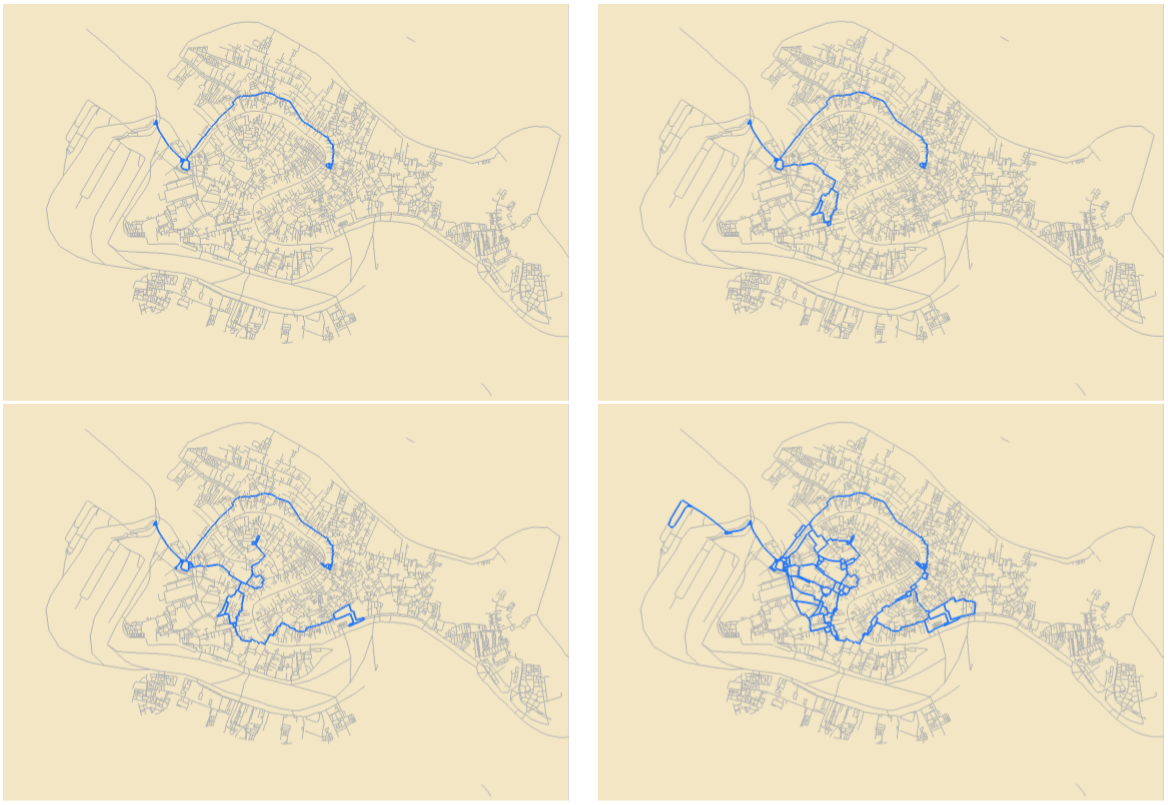
\includegraphics[width=0.85\textwidth]{venice_step.png}
\caption{From top-left to right-bottom, we plot four mobility subnetworks with increasing number of roads, selected by the \textsf{DNetPRO} algorithm using the Carnival dataset.
}
\label{fig:venice_step}
\end{figure}
\end{center}

Starting from the previously evaluated daily flows for each road, we order in a decreasing way the roads according to the observed
flows.
The \textsf{DNetPRO} algorithm scrolls down the list adding the road to a temporary list.
At every step the \quotes{pruning process} starts on the selected roads cutting the isolated roads in order to get a connected subnetwork\footnote{
  Since we are interested on the largest connected component the \emph{merging} parameter is off.
}.
Therefore the number of nodes of the subnetwork increases in a discontinuous way, when the adding of a new road in the list allows to
connect several previously selected roads.
After several parametric scans, we found that the best result for our purposes is achieved by choosing about the 10\% of the nodes in the whole Venice road network.
In Fig~\ref{fig:venice_step} we show four consecutive selected subnetworks in the case of Carnival dataset to illustrate how the algorithm operates.

\begin{center}
\begin{figure}[htbp]
\centering
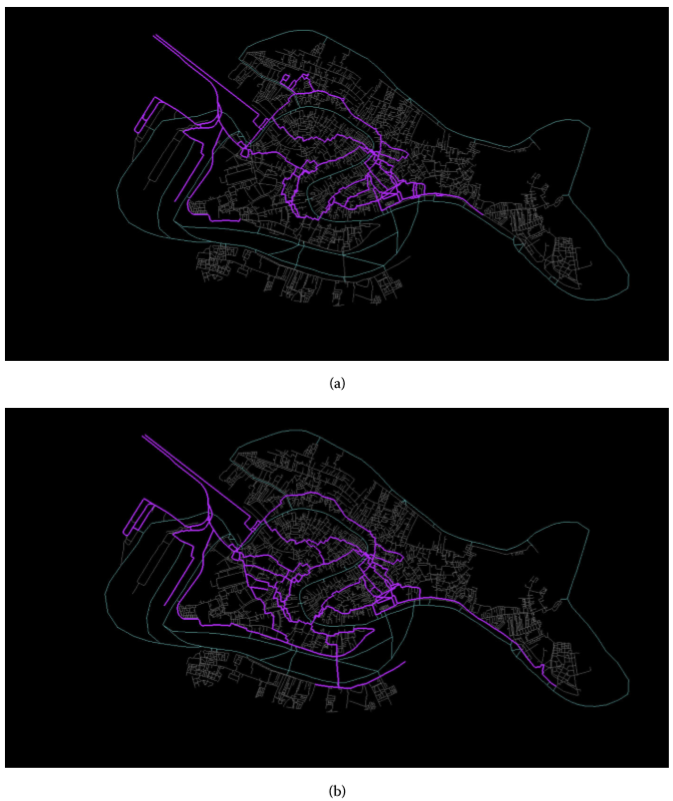
\includegraphics[width=0.85\textwidth]{venice_result.png}
\caption{Picture (a): selected subnetworks (highlighted in purple) from the road network of the Venice historical centre (in the background), that explain 64\% of the recorded mobility in the datasets.
The top picture refers to the Carnival mobility during 26/02/2017 and corresponds to 13\% of the total length of the Venice road network.
The picture (b) refers to the \emph{Festa del Redentore} mobility during 15/07/2017 and corresponds to 15\% of the total length of the Venice road network.
}
\label{fig:venice_result}
\end{figure}
\end{center}

Using the \textsf{DNetPRO} algorithm we are able to extract a subnetwork which explains the 64\% of the observed mobility using 13\% of the total road network length for the case of the Carnival dataset and 15\% of the total length in the case of the \emph{Festa del Redentore} dataset.

The selected road subnetworks are plotted in Fig~\ref{fig:venice_result} for both the datasets.
As a matter of fact, many of the highlighted paths are also suggested by Internet sites.
However, we remark some differences that can be related by the different nature of the considered events.
During the Carnival of Venice the mobility seems to highlight three main directions connecting the railway station and the \emph{Piazzale Roma} (top-left in the map), which are the main access points to the Venice historical centre, with the area around San Marco square, where many activities where planned during 26/02/2017.
In the case of the \emph{Festa del Redentore} the structure is more complex due to the appearance of several paths connecting the station and \emph{Piazzale Roma} with the \emph{Dorsoduro} district in front of the \emph{Giudecca} island.

This geometrical structure could have a double explanation: on one hand the \emph{Festa del Redentore} introduces an attractive area near the \emph{Giudecca} island, where the fireworks take place in the evening; on the other hand the \emph{Festa del Redentore} is a festivity very much felt by the local population, that knows the Venice road network and performs alternative paths.

On these subnetwork we also map the mobility of Italians and foreigns separately.
The results of this application are deeply discussed in the paper.

\end{document}



\documentclass{standalone}

\begin{document}

\chapter*{Appendix C - BlendNet}\addcontentsline{toc}{chapter}{Appendix C - BlendNet}
\markboth{Appendix C}{BlendNet}

\begin{figure}[htbp]
\centering
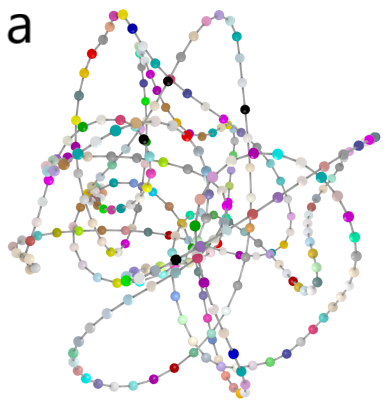
\includegraphics[width=0.4\textwidth]{cycle_graph.png}
\qquad\qquad
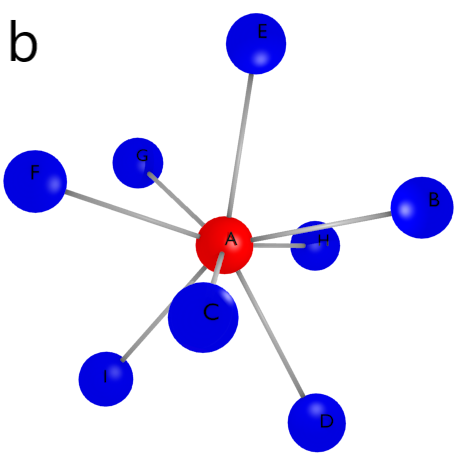
\includegraphics[width=0.4\textwidth]{star_graph_node.png}
\caption{(\textbf{a}) Chain graph example rendered by BlendNet software.
Node colors are random generated by the tool.
(\textbf{b}) Star graph example rendered by BlendNet software.
Node colors and labels are given as extra columns in node-list file.
}
\label{fig:blendnet}
\end{figure}

Graph visualization is still an open problem in many applications.
Commonly the problem is related to large graph visualization in which problems arise from the rendering of a large number of nodes and a greater number of links between them.
An other open problem concern the multi-dimensional visualization of the graphs.
Despite the most common graph tools compute the node coordinates in a any space dimensions (and clearly the maximum number of possible dimension for a visualization is still three) the real visualization is often allowed only a 2D space.
The counterpart of these problems concern the pretty visualization of the graphs that it is often ignored in many tools but it can be guarantee a good result, the so called wow-effect, in a presentation.

In this section we introduce a new custom graph viewer developed for pretty small network visualization in 2D and 3D called \emph{BlendNet}~\cite{BlendNet} (\emph{Blender Network viewer}).
BlendNet is open-source and it is released under GPL license.
All the small-graphs showed in this work are made using this tool and in particular the feature-signature generated by the DNetPRO algorithm.

BlendNet is a custom tool written in Python with the help of Blender API.
Blender is now a standard in the 3D rendering and it is commonly used in a wide range of graphical applications, starting from the simpler 3D dynamics to the video-games applications.
Blender is certainly more than a simple graphical viewer but the easy Python interface and the wide on-line documentation and blogs make it a useful tool for graphical representation of 3D structures.

To use the Blender API we are forced to use the Python version installed inside software and any extra-package required by our application have to be installed with the appropriate \textsf{pip}.
In our case we base our viewer on the \textsf{networkx} library for the computation of the possible node coordinates so we have to update our Python-Blender.
Moreover since the code can be difficult to manage for non-expert users we create an easy user command-line interface to set the whole set of parameters required by the graph visualization that can be piloted by \emph{Makefile} rules.
The list of nodes and edges can be passed via command-line filename in the same format of the concurrent graph viewer (e.g \emph{Gephi} software, the other graph viewer used in this work to generate the largest network structure of the CHIMeRA project).

The software project is a single script file and it includes a full list of possible examples and usages of the software.
Some of this examples are shown in Fig.~\ref{fig:blendnet}.
A full list of installation instructions is also given for any operative system (Unix, MacOS and Windows).
These instructions cover a full installation of Blender, Python and BlendNet package either for admin users either for no-root users~\cite{Shut}.
With slight modifications of the code we can obtain different nodes coordinates and a node shapes.
Nodes color, size and position can also be given in the node-list file as independent columns.

\end{document}


\documentclass{standalone}

\begin{document}

\chapter*{Appendix D - Multi-Class Performances}\addcontentsline{toc}{chapter}{Appendix C - Multi-Class Performances}
\markboth{Appendix D}{Scorer}

\begin{center}
\begin{figure}[htbp]
\centering
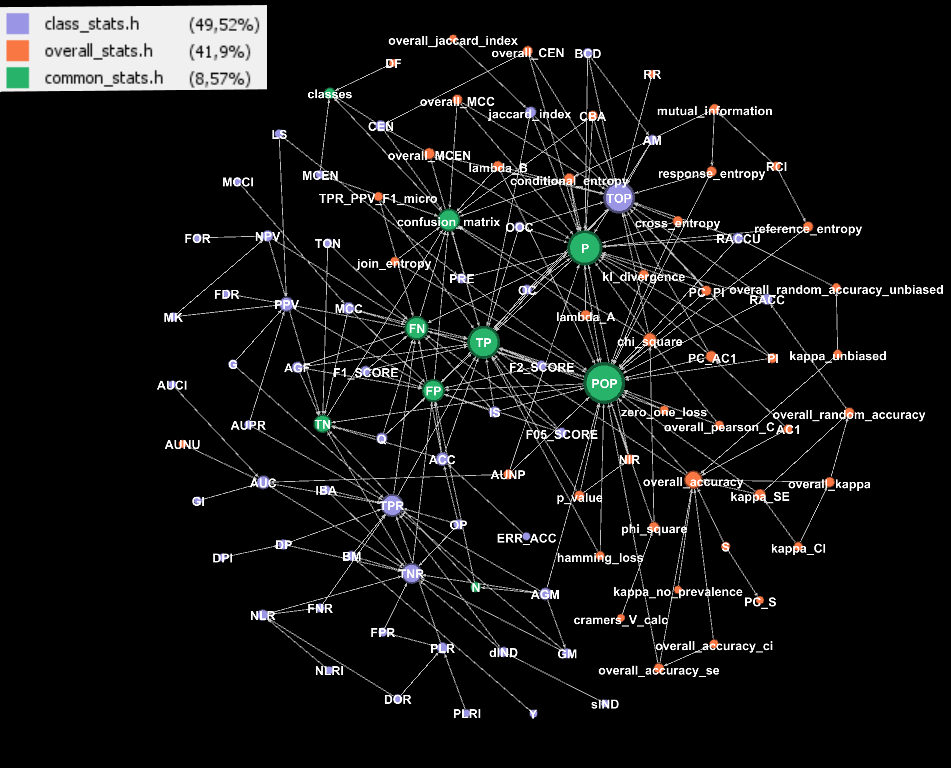
\includegraphics[width=0.6\textwidth]{scorer_net.png}
\caption{Multi class score interaction graph.
Each node identify a different performance evaluator and link are given by the interaction between the mathematical formulation of each quantity.
The graph has more than 100 nodes and more than 200 links.
The node colors are given by the classes identified in the work of Sepand et al.~\cite{PyCM}.
}
\label{fig:scorer_net}
\end{figure}
\end{center}

The evaluation of performances is a crucial task in any Machine Learning application.
Given a set of pattern and its corresponding (true) labels we can evaluate the efficiency of the understudy model with a comparison between them and the output of the model, i.e the predicted labels.
There are a lot of different scores that can be computed and any of them evaluate some aspects of the model efficiency.
Any paper author chose the score that better highlight the advantages of its model and it is difficult to move around this large zoo of indicators.
Moreover (it is quite a constant in scientific research) when a paper is send to a peer-review in many cases the reviewer suggests to the author to check if other performance indicators are good enough for the showed results.
This means that a lot of large simulations should be performed again and the appropriated variables re-computed to obtained the requested score.

At this point the main question is: are these scores totally independent one from each other?
The brief answer is simply no.
In a very interesting work of Sepand et al.~\cite{PyCM} they show how we can compute the wide part of these scores starting from the evaluation of the simple confusion matrix\footnote{
  The confusion matrix is a square matrix of shapes $(N, N)$, with $N$ the total number of classes in the current problem, whose entries are the number of rights and false classification.
  In particular, each entry of the matrix represents the instances predicted in a given class.
  If the class is the right one we call it a true positive item.
  As counterpart we will have a false positive item.
}.
Sepand et al. provide a full mathematical documentation and references about the computation of this wide range of scores starting from the evaluation of the confusion matrix.

Despite the Python code provided by Sepand et al. explain this links between the mathematical quantities they stop their analysis on the scores evaluation without any interest on the optimization of these computations.
Starting from their work we can analyze the inter-connections between these mathematical formulas and extract the dependencies between the involved variables.
In particular, a score quantity can be interpreted as a node and its connections are given by the variables needed to evaluate it.
Graphs of this type are commonly called \href{https://en.wikipedia.org/wiki/Factor_graph}{\emph{factor graphs}}.
In a mathematical formulation of \emph{factor graphs} there are different kinds of nodes (variables and factors, or equations).
The focus of our analysis is not on mathematical formalism of these kind of graphs but on the visualization of the functions interaction and on the results that we can obtain from it.

In the work of Sepand et al. the authors identify three classes of functions: common statistics, class statistics and overall stats, respectively.
In Fig.~\ref{fig:scorer_net} the interaction graph of these three classes is shown.
The figure shows deeper interactions between the three classes of functions and highlights the dependencies of the different quantities.
We can also use this kind of visualization to formulate computational considerations about the order in which compute these quantities.
Since the graph is a direct graph by definition, we can start from the root node (the node without links which bring to it) and cross the network until the leaf nodes (nodes without link which go out from the node) like in a tree-graph.
At each step of the percolation the incoming nodes identify totally independent quantities.
This independences means that the node-quantities can be potentially computed in parallel.
To clarify this considerations we can re-organize the graph visualization minimizing the link lengths and obtain a stratified graph in which each level identifies a potentially parallel section.
A graph with these properties can be obtained using the \textsf{dot} visualization and it is shown in Fig.~\ref{fig:scorer_parallel}.
As can be seen in the figure we can identify 7 levels in the graph and so 7 potentially parallel regions for the computation of the full set of functions.

\begin{center}
\begin{figure}[htbp]
\hspace{-2cm}

\includegraphics[width=1.3\textwidth]{scorer_parallel.pdf}
\caption{Re-organization of the graph in Fig.~\ref{fig:scorer_net}.
The rendering was obtained using the \textsf{dot} visualization, i.e the minimization of the link lengths.
The direct graph identifies the tree of dependencies and each level of the tree represents a set of independent functions that can be potentially computed in parallel.
This graph is used as parallel scheme for the \textsf{Scorer} library.
}
\label{fig:scorer_parallel}
\end{figure}
\end{center}

These considerations allow the creation of the optimized version of the code of Sepand et al., the \textsf{Scorer} library~\cite{Scorer}.
The \textsf{Scorer} library is the \textsf{C++} porting of the \textsf{PyCM} library of Sepand et al. with a \textsf{Cython} wrap for the \textsf{Python} compatibility.
Following the pre-told graph the computation of the score quantities are performed in parallel according to the levels of the tree-graph in Fig.~\ref{fig:scorer_parallel}.
The parallelization strategy chosen uses the \textsf{section} keyword of OpenMP library to perform no-wait task that are computed by each thread of the parallel region.

The graph covers more than 100 different quantities so writing the full set of parallel sections becomes an hard work in \textsf{C++}.
Moreover the updating of the graph with new quantities requires the updating of the full code and also of the parallelization strategy.
Each function was written as an anonymous-struct, i.e a functor, with an appropriate operator overloading.
Moreover each functor has a name given by a pre-determined regex (\textsf{get\_\{function\}}) and the list of argument follows the same nomenclature\footnote{
  If the functor receives in input the variable $A$ and $B$ we have to ensures that two functors named $get\_A$ and $get\_B$ will be provided.
  The only exception is given by the root functor.
}.
With these expedients we created a fully automated creation of the \textsf{C++} script which parses the list of above functors, it computes the dependency graph and the parallelization levels and give back a compilable \textsf{C++} script with the desired characteristics.
In this way we can guarantee an easy way to update the library and moreover we overcome the boring writing of a long code.
The automatic pipeline creation script is provided in the \textsf{Scorer} library and can be used at each pull request or version update.

For a pretty/useful visualization of the computed quantities we render the interaction graph in an HTML framework.
In this way in each node we can insert with a CSS table the computed values that can be discovered passing the mouse over the figure.
An example of this rendering is given in the on-line version of the library~\cite{Scorer}.

In conclusion the developed \textsf{Scorer} library is a very powerful tool for Machine Learning performances evaluation which can be used either in \textsf{C++} either in \textsf{Python} codes through the \textsf{Cython} wrap.
The code is automatically generated at each update and automatically tested using Continuous Integration for any platform\footnote{
  We perform tests for Unix and Windows environments.
  We check more than 15 combinations of environments and compilers.
}.
The code can be compiled using \textsf{CMakefile} or \textsf{Makefile} and a setup is provided for the \textsf{Python} version.
So when you write a new paper on Machine Learning and you do not know what could be the most appropriate indicator to show in your research or you are afraid that a referee could ask you to compute an other one there is only one solution: compute them all using \textsf{Scorer}.


\end{document}


\documentclass{standalone}

\begin{document}

\chapter*{Appendix E - Neural Network as Service}\addcontentsline{toc}{chapter}{Appendix E - Neural Network as Service}
\markboth{Appendix E}{Neural Network as Service}

One of the final goals of Machine Learning is certainly the process automation.
We develop everyday complex models to perform tasks that should be automatically executed by a computer without human supervision.
Neural Networks are classical mathematical tools used for these purposes and we have widely discussed about them in Chapter~\ref{chapter2:neural} of this work.
Beyond Neural Network structures and purposes for which they are made there is still an uncovered topic to discuss: the automation of these kind of algorithms into a computer device.
In this section we are going to discuss an implementation of these algorithms as service in a computer server.
In particular we will talk about the implementation of the \emph{FiloBlu} service which is part of a project developed in collaboration with the Sapienza University (Rome) and the INFN Data Center CNAF of Bologna.
This work is still in progress and its purpose goes beyond the current topic, so we will focus only on the implementation of the service without any reference on the Machine Learning algorithm used.
This is a further proof that the developed techniques are totally independent by the final application purpose.

A service is a software that is executed in background in a machine.
In Unix machines it is often call \textsf{daemon}s, while in Windows machine is called \emph{Windows service}.
A service starts only with administrator privileges and it goes on without any user presence.
An other important requirement is the ability to restart when some troubles occur in the machine functionality and/or at the boot of the machine.

A Machine Learning service could be used for applications in which we have to manage an asynchronous stream of data for long time intervals.
An example could be the case in which the data provider is identified by an App or a video-camera.
These data should be stored inside a central database that can be located in a different device or in the same computer in which the service run.
Since the service runs in background the only communication channel with the user is given by log files.
A log file is a simple readable file in which are saved the base informations about the current status of the service.
Thus, it is crucial to set appropriated check-points into the service script and chose the minimum quantity of informations that the service should write to make user-understandable its status.

\end{document}

\documentclass{standalone}

\begin{document}


\section*{FiloBlu Service}\addcontentsline{toc}{section}{FiloBlu Service}
\markboth{Appendix E}{FiloBlus Service}

In the \emph{FiloBlu} project we have a stream of data provided by an external App that are stored in a central database server.
The Machine Learning service has to read the information in the database, to process them and finally write the results in the same database.
All these operations have to be performed with high frequency since the result of the algorithm are shown in a real-time application.
This frequency will be the clock-time of the process function, i.e at each time interval (as small as we like) the process task will be called and we have the desired results in output.
At the same time we have to be care of the time required by our Machine Learning algorithm: not all the algorithms can process data in real time and the process function frequency has to be less than the time required by the algorithm or we can lose some frequency clock.

The best efficiency by a service can be obtained splitting as much as possible the required functionality in small-and-easy tasks.
Small task can evaluated as independent functions with an associated frequency that in this case can be reduced as much as possible.
The \emph{FiloBlu} required functionality can be reviewed as a sequence of 3 fundamental steps and other 2 optional ones: read the data from the database, process the data with the Machine Learning algorithm and write the obtained results on the database are certainly the fundamental ones; update the Machine Learning model and clear old log files are optional steps.
To further improve the efficiency of the service we can give each independent step to a different thread.
The whole set of tasks will be piloted by a master thread given by the service itself.
In this way the service will be computational efficient and moreover it does not weight on the computer performances.
We have always take in mind that the computer which host the service have to be effected by the daemon process as less as possible either in memory either on computational point-of-view.
Now we only have to synchronize our steps with appropriate clock frequencies.

Let's start from the reading data function.
Since our data are assumed to be stored in a database this function have to perform a simple query and extract the latest data inserted.
Obviously the efficiency of the step is based on the efficiency of the chosen query.
The data extracted will be saved in a common container shared between the list of thread and thus belonging to the master.
The choice of an appropriate shared container is a second point to carefully take in mind.
This container should be light an thread-safe to avoid thread concurrency.
While the second request is implementation dependent the first one can be faced on using a FIFO container\footnote{
  FIFO container, i.e \emph{First-In-First-Out}, is a special data structure in which the first element added will be processed as first and then automatically removed from it.
}.
In this way we can ensure that the application will saved a fixed maximum of data and it will not occupy large portion of memory (RAM).

The second task is identified by the Machine Learning function which process the data.
The algorithm will take from the FIFO container of the previous step (if there is) and it will save the result in a second FIFO container for the next step.
The time frequency of the step is given by the time required by the Machine Learning algorithm.

The third step will keep the data from the FIFO container of results (if there is) and it performs a second query (a writing one in this case) to the database.
Also in this case the frequency is given by the efficiency of the chosen query.

The last two steps can be executed without press time requirements and are useful only on a large time scale.

Each step perform its independent logging on a single shared file.
If an error occurs the service logs the message and save the current log-file in a different location to prevent possible log-cleaning (optional step).
Then the service will be re-started.

% \begin{figure}[htbp]
% \centering
% \def\svgwidth{0.8\textwidth}
% \input{./img/FiloBlu.pdf_tex}
% \caption{
% }
% \label{fig:FiloBlu}
% \end{figure}

%The above computational scheme of the service is shown in Fig.~\ref{fig:FiloBlu}.

We implemented this type of service in pure Python~\cite{FiloBlu}.
The developed service was customize according to the server requirements of the project\footnote{
  The FiloBlu service is a Windows service and it can not run on Unix machines.
  Moreover the database used in the project is a MySQL one so the queries and the libraries used are compatible only with this kind of databases.
}.
We chose the Python language either for its simplicity in the code writing either for its thread native module which ensures a total thread-safety of each variable.
Using simple decorator we are able to run each function in a separate-detached thread as required by the previous instructions.
The project includes a documentation about its use (also in general applications) and it can be easily installed via \textsf{setup}.
In the \emph{FiloBlu} project we use a Neural Network algorithm written in \emph{Tensorflow}.
\emph{Tensorflow} does not allow to run background process directly so the problem was overcame using a direct call to a Python script which perform full list of steps into an infinite loop.
In this way the service can be re-started also if the process-service is killed.
The service can be driven using a simple \emph{Powershell} script provided in the project.

\end{document}

\documentclass{standalone}

\begin{document}

\section*{Data Transmission}\addcontentsline{toc}{section}{Data Transmission}
\markboth{Appendix E}{CryptoSocket}

In the above configuration we focused on the pipeline which process the stream of data ignoring any problem about the communication between the external device and the machine which host the service.
The \emph{FiloBlu} project uses an external APP to send data to the main server, so we have two systems which have to communicate between them automatically via Internet connection.
In general, we could manage sensitive data that could be vulnerable using an Internet communication.
To face this problem we developed a simple TCP/IP client-server package which also supports a RSA cryptography, the \textsf{CryptoSocket} package~\cite{CryptoSocket}.

The communication security could be an important point in many research applications and a valid cryptography procedure is essential.
The RSA cryptography is considered one of the most secure cryptography algorithm for data transmission and it is quite easy to implement.
In the \textsf{CryptoSocket} package we implemented a simple wrap around the \textsf{socket} \textsf{Python} library to perform a serialization of our data which are (optionally) processed by our custom \href{https://en.wikipedia.org/wiki/RSA_(cryptosystem)}{RSA algorithm}.
In this way different kind of data could be sent by the client at the same time.
The \href{https://github.com/Nico-Curti/CryptoSocket/blob/master/CryptoSocket/examples/client.py}{client} script could be adapted with slight modifications for any user need and also complex \textsf{Python} structures could be transmitted between two machines (to the \href{https://github.com/Nico-Curti/CryptoSocket/blob/master/CryptoSocket/examples/server.py}{server}).
The cryptography module was written in pure \textsf{C++} for computational efficiency and a \textsf{Cython} wrap was provided for pure-\textsf{Python} applications.
\textsf{CryptoSocket} has only demonstrative purpose and so it works only for a 1-by-1 data transmission (1 server and 1 client).

Since this second implementation could be used also for other applications it was treated as a separated project and it has its own open-source code.
The \textsf{CryptoSocket} package can be installed via \href{https://github.com/Nico-Curti/CryptoSocket/blob/master/CMakeLists.txt}{\textsf{CMake}} in any platform and operative system and a full list of installation instructions is provided in the project repository.
The continuous integration of the project is guaranteed by testing the package installation across multiple \textsf{C++} compilers and platforms via \href{https://github.com/Nico-Curti/CryptoSocket/blob/master/.travis.yml}{Travis CI} and \href{https://github.com/Nico-Curti/CryptoSocket/blob/master/appveyor.yml}{Appveyor CI}.

\end{document}



\documentclass{standalone}

\begin{document}

\chapter*{Appendix F - Bioinformatics Pipeline Profiling}\addcontentsline{toc}{chapter}{Appendix F - Bioinformatics Pipeline Profiling}
\markboth{Appendix F}{Profiling}

In this work many times we have talked about the performances evaluation of a scripts in terms of time performances and other system statistics.
The importance in the understanding the state of our infrastructure is essential not only for ensuring the reliability and stability of a software but also for a more efficiency use of the available resources.
In particular about what concern the memory, CPUs and diskIO management is useful to know the required amount of each step of our software to perform the better parallelization strategy.
Metrics represent the raw measurements of resource usage that are used by a software or a collection of them.
These might be low-level usage summaries provided by the operating system, or they can be higher-level types of data tied to the specific functionality or work of a component.
These kind of data could be collected and aggregated by a monitoring system like \href{https://github.com/influxdata/telegraf}{\emph{Telegraf}}\footnote{
  An automatic installation guide for Telegraf is provided in the Shut~\cite{Shut} project for any OS and also for no-root users.
}.
In general, the difference between metrics and monitoring mirrors the difference between data and information.
Monitoring takes metrics data, aggregates it, and presents it in various ways that allow humans to extract insights from the collection of individual pieces.

In this section we focused on the importance of software monitoring.
In particular we will talk about a work conducted in collaboration with INFN-CNAF of Bologna about the monitoring and the performance evaluation of a bioinformatics pipeline across various computational environments~\cite{EuroPar2018}.

In this work a previously published bioinformatics pipeline was reimplemented across various computational platforms, and the performances of its steps evaluated.
The tested environments were:
I) dedicated bioinformatics-specific server
II) low-power single node
III) HPC single node
IV) virtual machine.
The pipeline was tested on a use case of the analysis of a single patient to assess single-use performances, using the same configuration of the pipeline to be able to perform meaningful comparison and search the optimal environment/hybrid system configuration for biomedical analysis.
Performances were evaluated in terms of execution wall time, memory usage and energy consumption per patient.

\end{document}

\documentclass{standalone}

\begin{document}


\section*{GATK-LODn pipeline}\addcontentsline{toc}{section}{GATK-LODn pipeline}
\markboth{Appendix F}{GATK-LODn}

\begin{table*}
\centering
\begin{tabular}{lccccc}
\hline \rowcolor{darkgrayrow}
                      & \textbf{Coverage} & \textbf{No. of} & \textbf{Read}   & \textbf{BAM file} & \textbf{NGS}  \\
\rowcolor{darkgrayrow}
                      &                   & \textbf{Reads}  & \textbf{Length} & \textbf{size}     & \textbf{size} \\
\hline
\textbf{Whole genome} & 37.7x             & 975,000,000     & 115             & 82 GB             & 104 GB        \\

\textbf{Whole genome} & 38.4x             & 3,200,000,000   & 36              & 138 GB            & 193 GB        \\

\textbf{Exome}        & 40x               & 110,000,000     & 75              & 5.7 GB            & 7.1 GB        \\
\hline\\
\end{tabular}
\caption{Typical dataset size for a single patient of different types of next generation sequencing.
BAM file size refers to the size of the binary file containing the reads from the machine.}
\label{fig:wes_datasize}
\end{table*}

The pipeline used in this work, GATK-LODn, has been developed in 2016 by Do Valle et al.~\cite{DoValle2016}, and codifies a new approach aimed to Single Nucleotype Polimorphism (SNP) identification in tumors from Whole Exome Sequencing data (WES).
WES is a type of \quotes{next generation sequencing} data~\cite{Zwolak2008, Behjati2013, Shendure2008}, focused on the part of the genome that actually codifies proteins (the exome).
Albeit known that non-transcriptional parts of the genome can affect the dynamic of gene expression, the majority of cancers inducing mutations are known to be on the exome, thus WES data allow to focus the computational effort on the most interesting part of the genome.
Being the exome in human approximately 1\% of the total genome, this approach helps significantly in reducing the number of false positives detected by the pipeline.
The different sizes of next generation sequencing dataset are shown in Tab~\ref{fig:wes_datasize}.

The GATK-LODn pipeline is designed to combine results of two different SNP-calling softwares, GATK~\cite{McKenna2010} and MuTect~\cite{Cibulskis2013}.
These two softwares employ different statistical approaches for the SNP calling: GATK examines the healthy tissue and the cancerous tissue independently, and identifies the suspect SNPs by comparing them; Mutect compares healthy and cancerous tissues at the same time and has a more strict threshold of selection.
In identifying more SNPs, GATK has a higher true positive calling than Mutect, but also an higher number of false positives.
On the other end Mutect has few false positives, but often does not recognize known SNPs.
The two programs also call different set of SNPs, even when the set size is similar.
The pipeline therefore uses a combination of the two sets of chosen SNPs to select a single one, averaging the strictness of Mutect with the recognition of known variants of GATK.

The pipeline work-flow includes a series of common steps in bioinformatics analysis and in the common bioinformatics pipelines.
It includes also a sufficient representative sample of tools for the performances statistical analysis.
In this way the results extracted from the single steps analysis could be easily generalized to other standard bioinformatics pipelines.

With the increasing demand of resources from ever-growing datasets, it is not favorable to focus on single server execution, and is better to distribute the computation over cluster of less powerful nodes.
The computational pipeline also has to manage a high number of subjects, and several steps of the analyses are not trivial to be done in a highly parallel way.
Thus, the importance of system statistics management as the efficiency usage of available resources are crucial to reach a compromise between computational execution time and energy cost.
For these reasons our main focus is on the performance evaluation of a single subject without using all the available resources, as these could be more efficiently allocated to concurrently execute several subjects at the same time.
Due to the nature of the employed algorithms, not all steps can exploit the available cores in a highly efficient way: some scales sub-linearly with the number of cores, some have resource access bottleneck.
Other tools are simply not implemented with parallelism in mind, often because they are the result of the effort of small teams that prefer to focus their attention on the scientific development side rather than the computational one.

Moreover in order to obtain an optimal execution of bioinformatics pipelines, each analysis step might need very different resources.
This means that any suboptimal component of a server could act as a bottleneck, requiring bleeding edge technology if all the steps are to be performed on a single machine.
Hybrid systems could be a possible solution to these issues, but designing them requires detailed information about how to partition the different steps of the pipeline.

\end{document}

\documentclass{standalone}

\begin{document}


\section*{Computational Environments}\addcontentsline{toc}{section}{Computational Environments}
\markboth{Appendix F}{Computational Environments}

\begin{figure*}
\centering
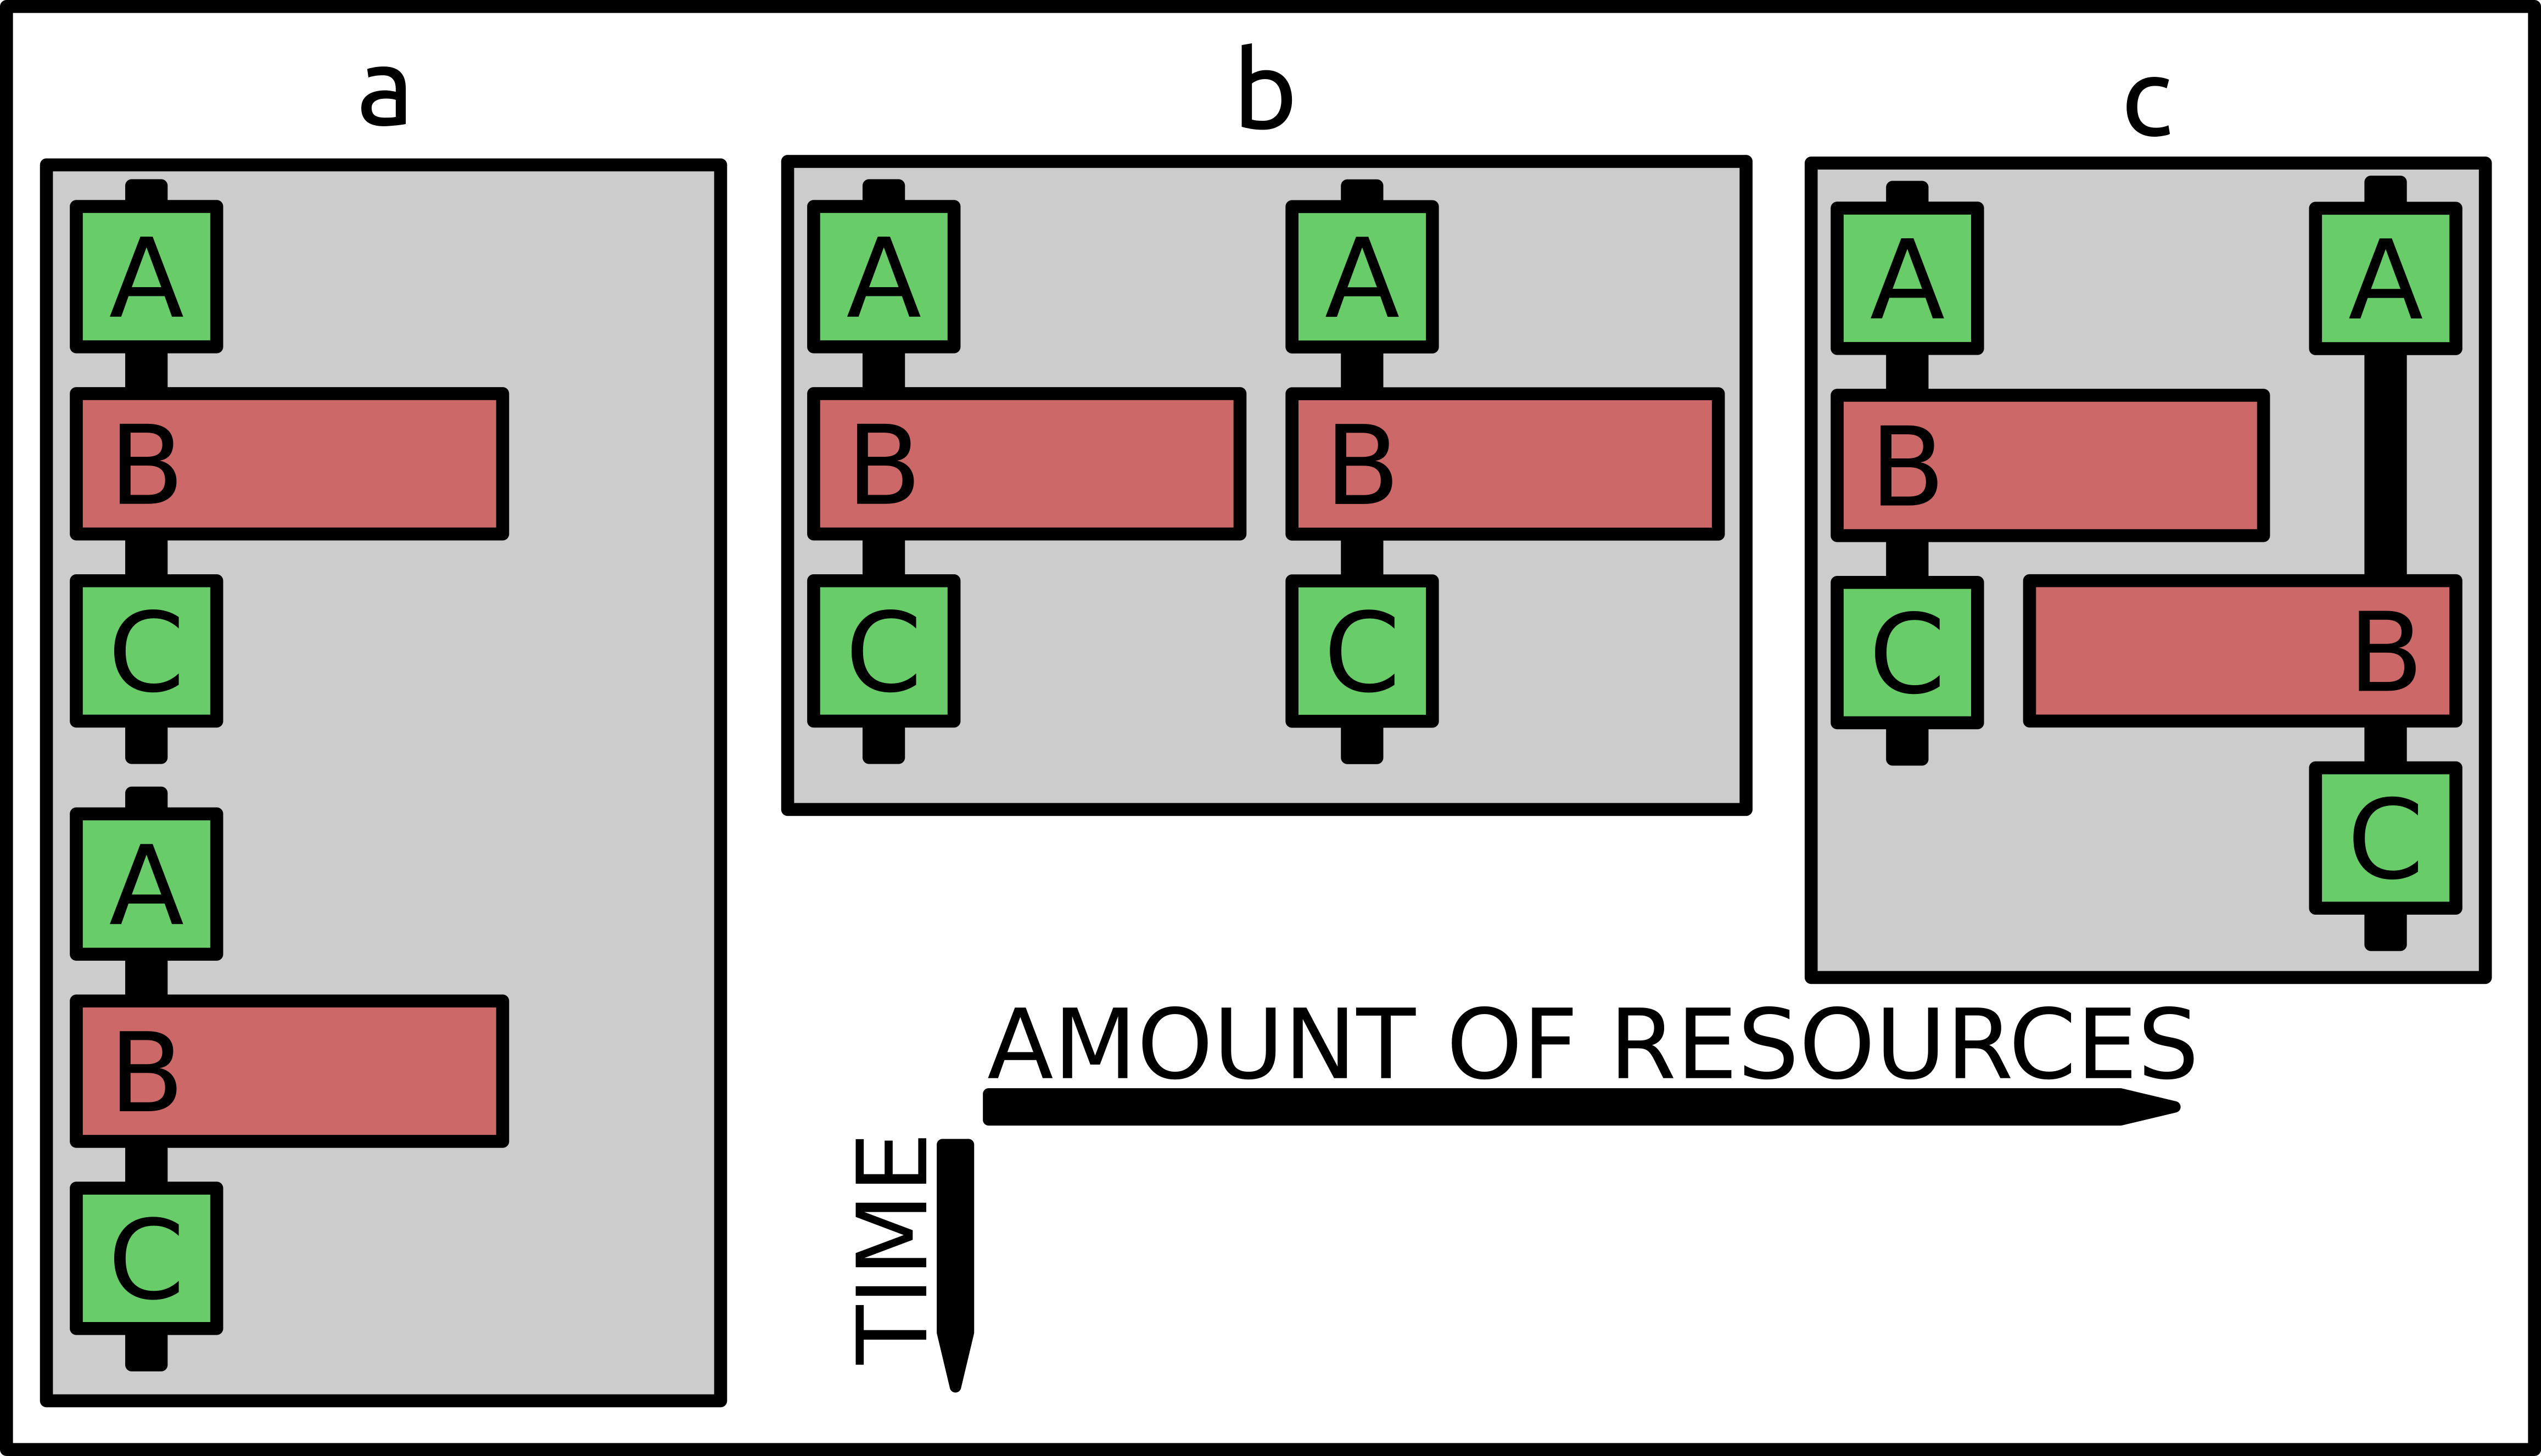
\includegraphics[width=.6\linewidth]{concurrency.png}
\caption{Examples of concurrency work-flow of two processes.
The first case ($a$) represents a simple (naive) sequential work-flow; the second ($b$) highlights a brute force parallelization; the third ($c$) is the case of a perfect match between the available resources and the requested resources.
Often brute force parallelization of pipelines done as in the image $b$ ends up overlapping the most computationally intensive steps.
Measuring the minimum viable requirements for the execution allow to better allocate resources as seen in the image $c$.}
\label{fig:wes_concurrency}
\end{figure*}

There are two main optimization strategies: the first is to improve the efficiency of a single run on a single patient and the second is to employ massive parallelization on various samples.
In both cases we have to know the necessary resources of the pipeline (and in a fine grain the resources of each step) and the optimal concurrency strategy to be applied to our work-flow (see Fig.~\ref{fig:wes_concurrency}).
In the analyses we want to highlight limits and efficiencies of the most common computational environments used in big data analytics, without any optimization strategy of the codes or systems.

We also focused on a single patient analysis, the base case study to design a possible parallelization strategy.
This is especially relevant for the multi-sample parallelization, that is the most promising of the two optimization strategies, as it does not rely on specific implementations of the softwares employed in the pipeline.

The pipeline was implemented on 5 computational environments: 1 server grade machine (Xeon E52640), 1 HPC node (Xeon E52683), 2 low power machines (Xeon D and Pentium J) and one virtual machine built on an AMD Opteron hypervisor.
The characteristics of each node are presented in Tab.~\ref{tab:node-characteristic}.

The server~-~grade node is a typical node used for bioinformatics computation, and as such features hundreds of GB of memory with multiple cores per motherboard: for these reasons we chose it as reference machine and the following results are expressed in relation to it.

The two low~-~power machines are designed to have a good cost~-~to~-~performance ratio, especially for the running cost\footnote{
  Running cost is evaluated as the energy consumption that the node requires per subject, assuming that the consumption scales linearly with the number of cores used in the individual step.
}.
These machines have been proven to be a viable solution for high performance computations~\cite{Cesini2017}.
Their low starting and running cost mean that a cluster of these machines would be more accessible for research groups looking forward to increase their computational power.

The last node is a virtual machine, designed to be operated in a cloud environment.

The monitoring tool used is \emph{Telegraf}, which is an agent written in Go for collecting, processing, aggregating, and writing metrics.
Each section of the pipeline sends messages to the \emph{Telegraf} daemon independently.

Regardless of the number of cores of each machine we restrict the number of cores used to only two to compare the statistics: this restriction certainly penalize the environment with multiple cores but with a view of maximizing the parallelizations and minimize the energy cost it is the playground to compare all the available environments.
Another restriction is applied to the chosen architectures: since available low~-~power machines provides only x86~-~architectures also the other environments are forced to work in x86 to allow the statistics comparison.

\begin{table*}
\hspace{-.75cm}
\begin{tabular}{llllll}
\hline \rowcolor{darkgrayrow}
\textbf{CLASS} & \multicolumn{2}{c}{\textbf{server grade machines}} & \multicolumn{2}{c}{\textbf{low power machines}} & \textbf{virtual machine}\\
\hline
\textbf{CPU}      & Intel Xeon  & Intel Xeon  & Intel Pentium & Intel Xeon  & AMD Opteron \\
\textbf{version}    & E5-2683v3   & E5-2640v2   & J4205   & D-1540  & 6386 SE   \\
\textbf{Microarchitecture}  & Haswell   & Ivy Bridge EP & Apollo Lake   & Broadwell   & Piledriver  \\
\textbf{Launch Date}    & Q3'14   & Q3'13   & Q4'16   & Q1'15   & Q3'12   \\
\textbf{Lithography}    & 22 nm   & 22 nm   & 14 nm   & 14 nm   & 32 nm   \\
\textbf{Cores/threads}    & 14/28   & 8/16    & 4/4     & 8/16    & 16    \\
\textbf{Base/Max Freq}    & 2.00/3.00   & 2.00/2.50   & 1.50/2.60   & 2.00/2.60   & 2.80/3.50 \\
\textbf{L2 Cache}     & 35 MB   & 20 MB   & 2 MB    & 12 MB   & 16 MB   \\
\textbf{TDP}      & 120 W   & 95 W    & 10 W    & 45 W    & 115 W   \\
\textbf{Total CPUs}     & 2     & 2     & 1     & 1     & 1   \\
\textbf{total cores/threads}  & 28/56   & 16/32   & 4/4     & 8/16    & 16    \\
\textbf{Total Memory}     & 256 GB  & 252 GB  & 8 GB    & 32 GB   & 60 GB   \\
\textbf{System power}     & 240 + 60 W  & 190 + 60 W  & 10 + 2 W  & 45 + 10 W   & 115 + 10 W  \\
\textbf{Electrical costs}   & 650 €/year  & 550 €/year  & 26 €/year   & 120 €/year  & 273€ /year  \\
\textbf{System price}   & 4000-6000 €   & 3000-5000 €   & 100-130 €   & 900-1200 €  & 2000-3000€  \\
\hline\\
\end{tabular}
\caption{Characteristics of the tested computational environments.
Electrical costs are estimated as 0.25~€/kWh; CPU frequencies are reported in GHz; TDP: Thermal Design Power, an estimation indicator of maximum amount of heat generated by a computer chip when a \quotes{real application} runs.}
\label{tab:node-characteristic}
\end{table*}

\end{document}

\documentclass{standalone}

\begin{document}

\section*{Pipeline steps}\addcontentsline{toc}{section}{Pipeline steps}
\markboth{Appendix F}{Pipeline steps}

The pipeline steps that have been examined are a subset of all the possible steps: we only focus on those whose computational requirements are higher and thus require the most computational power.
These steps are:

\begin{enumerate}

\item\textbf{mapping:} takes all the reads of the subjects and maps them on the reference genome;

\item\textbf{sort:} sorts the sequences based on the alignment, to improve the reconstruction steps;

\item\textbf{markduplicates:} checks for read duplicates (that could be imperfections in the experimental procedures and would skew the results);

\item\textbf{buildbamindex:} indexes the dataset for faster sorting;

\item\textbf{indexrealigner:} realigns the created data index to the reference genome;

\item\textbf{BQSR:} base quality score recalibration of the reads, to improve SNPs detection;

\item\textbf{haplotypecaller:} determines the SNPs of the subject;

\item\textbf{hardfilter:} removes the least significant SNPs.

\end{enumerate}

The following statistics were evaluated:

\begin{enumerate}

\item\textbf{memory per function:} estimate percentage of the total memory available to the node used for each individual step of the pipeline;

\item\textbf{energy consumption:} estimated as the time taken by the step, multiplied by the number of cores used in the step and the power consumption per core (TDP divided by the available cores). As mentioned before this normalization unavoidably penalize the multi-core machines but give us a term of comparison between the different environment;

\item\textbf{elapsed time:} wall time of each step.

\end{enumerate}

The pipeline was tested on the patient data from the 1000 genome project with access code NA12878, sample SRR1611178.
It is referred as a Gold Standard reference dataset~\cite{Zook2014}.
It is generated with an Illumina HiSeq2000 platform, SeqCap EZ Human Exome Lib v3.0 library and have a 80x coverage.
As Gold Standard reference it is commonly used as benchmark of new algorithm and for our purpose can be used as valid prototype of genome.

\end{document}

\documentclass{standalone}

\begin{document}


\section*{Results}\addcontentsline{toc}{section}{Results}
\markboth{Appendix F}{Results}

Memory occupation is one of the major drawbacks of the bioinformatics pipelines, and one of the greater limits to the possibility of parallel computation of multiple subjects at the same time.
As it can be seen in Fig.~\ref{fig:memory-per-step}, the memory occupation is comprised between 10\% and 30\% on all the nodes.
This is due to the default behavior of the GATK libraries to reserve a fixed percentage of the total memory of the node.
The authors could not find any solution to prevent this behavior from happening.
As it can be noticed, in the node with the greatest amount of total memory (both Xeon E5 and the virtual machine) the requested memory is approximately stable, as is always sufficient for the required task.
The memory allocation is less stable in the nodes with a limited memory (Xeon D and Pentium J), as GATK might requires more memory than what initially allocated to perform the calculation.
The exception to this behavior is the \emph{mapping} step, that uses a fixed amount of memory independently from the available one (between 5 and 7 GB).
This is due to the necessity of loading the whole human reference genome (version hg19GRCh37) to align each individual read to it.
All the other steps do not require the human reference genome but can work on the individual reads, allowing greater flexibility in memory allocation.

As can be seen in Fig.~\ref{fig:performance-per-step} and Fig.~\ref{fig:energy-per-step}, this increase of memory consumption does not correspond to a proportional improvement of the time elapsed in the computation.

The elapsed time for each step and for the whole pipeline can be seen in Fig.~\ref{fig:performance-per-step}.
It can be seen that there is a non consistent trend in the behavior of the different environments.
Aside from the most extreme low power machine, the pentium J, the elapsed times are on average higher for the low power and slightly higher for the cloud node, but the time for the individual rule can vary.
In the sorting step, Pentium J is 20 times slower than the reference.
This is probably due to the limited cache and memory size of the pentium J, that are both important factors determining the execution time of a sorting algorithm and are both at least four to six times smaller than the other machines.
The HPC machine, the Xeon E52683, is consistently faster than the reference node.

The energy consumption per step can be seen in Fig.~\ref{fig:energy-per-step}.
The low power machines are consistently less than half the baseline consumption.
Even considering the peak of consumption due to the long time required to perform the sorting, the most efficient low power machine, the pentium J, consumes 40\% of the reference, and the Xeon D consumes 60\% of the reference.
The HPC machine, the Xeon E52683, have consumption close to the low power nodes, balancing out the higher energy consumption with a faster execution speed.
The virtual machine has the highest consumption despite the fact that the execution time of the whole pipeline is comparable to the reference due to the high TDP compared to its execution time.

\begin{figure*}[t!]
\centering
\def\svgwidth{\textwidth}
\input{./img/memory_per_function.pdf_tex}
\caption{Memory used for each step of the pipeline. Due to the GATK memory allocation strategy, all steps use a baseline amount of memory proportional to the available memory. Smaller nodes, like the low power ones, require more memory as the baseline allocated memory is not sufficient to perform the calculation.}
\label{fig:memory-per-step}
\end{figure*}

\begin{figure*}[t!]
\centering
\def\svgwidth{\textwidth}
\input{./img/time_performances.pdf_tex}
\caption{Time elapsed per step of the pipeline, and total elapsed time. In the sorting step, Pentium J is 20 times slower than the reference, probably due to the limited cache size.}
\label{fig:performance-per-step}
\end{figure*}

\begin{figure*}[t!]
\centering
\def\svgwidth{\textwidth}
\input{./img/energy_and_cost.pdf_tex}
\caption{Energy consumption per pipeline step and on the whole pipeline.
Energy consumption is estimated as the time taken by the step, multiplied by the number of cores used in the step and the power consumption per core (TDP divided by the available cores).
}
\label{fig:energy-per-step}
\end{figure*}


\end{document}

\documentclass{standalone}

\begin{document}


\section*{Conclusions}\addcontentsline{toc}{section}{Conclusions}
\markboth{Appendix F}{Conclusions}

Bioinformatics pipelines are one of the most important uses of biomedical big data and, at the same time, one of the hardest to optimize, both for their extreme requisites and the constant change of the specification, both in input-output data format and program API.

This makes the task of pipeline optimization a daunting one, especially for the final target of the results; physicians and biologists could lack the technical expertise (and time) required to optimize each new version of the various softwares of the pipelines.
Moreover, in a verified pipeline updating the software included without a long and detailed cross-validation with the previous one is often considered a bad practice: this means that often these pipelines are running with under-performing versions of each software.

Clinical use of these pipelines is growing, in particular with the rise of the concept of \quotes{personalized medicine}, where the therapy plan is designed on the specific genotype and phenotype of the individual patient rather than on the characteristic of the overall population.
This would increase the precision of the therapy and thus increase its efficacy, while cutting considerably the trial and error process required to identify promising target of therapy.
This requires the pipelines to be evaluated in real time, for multiple subjects at the same time (and potentially with multiple samples per subject).
To perform this task no single node is powerful enough, and thus it is necessary to use clusters.
This brings the need to evaluate which is the most cost and time efficient node that can be employed.

In the cost assessment there are several factors that need to be considered aside of the initial setup cost, namely cost for running the server and opportunity cost for obsolescence.
Scaled on medium sized facilities, such the one that could be required for a hospital, this cost could quickly overcome the setup cost.
This cost does also include not only the direct power consumption of the nodes, but also the required power for air conditioning to maintain them in the working temperature range.
Opportunity costs are more complex, but do represent the loss of possibility of using the most advanced technologies due to the cost of the individual node of the cluster.
Higher end nodes require a significant investment, and thus can not be replaced often.

With this perspective in mind, we surmise that energy efficient nodes present an interesting opportunity for the implementation of these pipelines.
As shown in this work, these nodes have a low cost per subject, paired with a low setup cost.
This makes them an interesting alternative to traditional nodes as a workhorse node for a cluster, as a greater number of cores can be bought and maintained for the same cost.

Given the high variability of the performances in the various steps, in particular with the sorting and mapping steps, it might be more efficient to employ a hybrid environment, where few high power nodes are used for specific tasks, while the bulk of the computation is done by the energy efficient nodes.
This is true even for those steps that can be massively parallelized, such as the mapping, as they benefit mainly from a high number of processors rather than few powerful ones.
In this work we focused only on CPUs computation, but another possibility could be an hybrid-parallelization approach in which the use of a single GPU accelerator can improve the parallelization of the slower steps.
Each pipeline work-flow requires its own analyses and tuning to reach the best performances and the right parallelization strategy based on the use which it is intended but a low energy node approach is emerging as a good alternative to the more expensive and common solutions.


\end{document}


\end{document}

% reference to the studies about performances of the developed algorithms.

%%%%%%%%%%%%%%%%%%%%%%%%%%%%%%%%%%%%%%%%%%%%%%%%%%%%%%%%
%\clearpage

%\documentclass{standalone}

\begin{document}

\chapter*{Relazione attività di ricerca}
\markboth{Relazione}{Relazione}

La prima parte del mio dottorato di ricerca si è svolto all'interno del gruppo di sistemi complessi (PhySyCom) dell'Università di Bologna, guidato dal prof. Bazzani.
Con il gruppo PhySyCom ho potuto approfondire le mie competenze algoritmiche e ho studiato approfonditamente le potenzialità dei linguaggi di programmazione a basso livello come il C e il C++.
Le mie competenze di programmazione sono state formate anche grazie alla partecipazione a \emph{Eighth I.N.F.N. International School on architectures, tools and methodologies for developing efficient large scale scientific computing applications} ed al workshop \emph{Intel-Code Modernization Workshop Rome}, durante i quali ho potuto studiare le tecniche di calcolo parallelo e distribuito.

Inizialmente mi sono occupato principalmente di analisi su dati di traffico automobilistico, forniti dalla regione Emilia Romagna, e su modelli a network, per l'ottimizzazione della rete peritale italiana di Unipol Assicurazioni, la quale ha finanziato il mio primo anno di dottorato.
Per quanto riguarda i dati di traffico, l'obiettivo del lavoro era quello di riuscire a predire, con sufficiente anticipo, l'insorgenza di ingorghi stradali e quindi procedere a dare "l'allarme" agli automobilisti.
Con questo progetto ho iniziato ad utilizzare e sviluppare i primi algoritmi di deep learning per l'analisi dati, i quali sono stati applicati fornendo buoni risultati, sui quali stiamo scrivendo un articolo.
Questi risultati sono stati presentati alla conferenza \emph{Problems in discrete dynamics: from biochemical systems to rare events, networks, clustering and related topics - II Edition} del 2017.
Il lavoro svolto con Unipol Assicurazioni, invece, pur avendo portato a buoni risultati non si è potuto concretizzare in una pubblicazione, vista la sensibilità dei dati coinvolti.
Nel mentre, in collaborazione con il centro INFN-CNAF, ho lavorato sull'ottimizzazione di una pipeline di bioinformatica, studiandone le performance di calcolo in termini di occupazione di memoria, tempistiche e consumi energetici.
Questo lavoro mi ha permesso di partecipare alla conferenza \emph{EuroPar2018} in cui ho presentato il mio lavoro e relativo articolo (\emph{Cross-Environment comparison of a bioinformatics pipeline: perspectives for hybrid computations}~\cite{EuroPar2018}.

A cavallo tra il primo e il secondo anno di dottorato ho iniziato a spostare la mia attività di ricerca su argomenti più attinenti al campo della biofisica e teoria dei network, lavorando con il gruppo Biophys dell'Università di Bologna, guidato dal prof. Castellani e dal prof. Remondini.
In particolare, ho iniziato a lavorare sulla ricostruzione della struttura 3D delle proteine a partire dalla relativa mappa di contatto.
Questo problema è stato da me affrontato mediante lo studio della matrice laplaciana associata al network e la relativa analisi spettrale.
Utilizzando gli autovettori della matrice laplaciana come coordinate degli amminoacidi, ho potuto ottenere buoni risultati, i quali però sono ancora in fase di revisione e non si sono ancora concretizzati in una pubblicazione.

Durante il secondo anno la mia attività di ricerca è stata finanziata dal progetto \emph{Venice}, svolto in collaborazione con il comune di Venezia, Canon Inc., Telecom Italia e Fabbrica Digitale.
Il progetto si proponeva di studiare il flusso pedonale all'interno della città di Venezia.
A questo scopo ho potuto ulteriormente approfondire le mie conoscenze sui modelli a rete neurale per l'object detection e studiare ulteriori tecniche di programmazione parallela.
In particolare, ho studiato e sviluppato reti feed forward a grande dimensionalità (es. Yolo, ImageNet, ResNet152, ...) e modelli a spin glass applicati a reti neurali (rFBP e rSGD).
Oltre alle basi teoriche di questi algoritmi, buona parte del mio lavoro è stato speso nell'implementare ed ottimizzare questi metodi mediante tecniche di calcolo parallelo multi-threading (OMP) e distribuito (MPI).
Per alcune applicazioni si è resa necessaria l'implementazione di kernel in CUDA e OpenCL per sfruttare acceleratori GPU.

Utilizzando una di queste reti a deep learning, implementata su schede Jetson TX2 con annesse telecamere, siamo riusciti a monitorare in tempo reale il flusso pedonale della città di Venezia, andando a contare (con anche informazioni direzionali sul moto) le persone all'interno di sequenze video.
In questo progetto mi sono occupato anche della gestione delle telecamere e della manutenzione del software da remoto, implementando pipeline che fossero in grado di eseguire questi compiti autonomamente.
Questo progetto è tuttora in corso, ma il mio contributo si è fermato all'analisi dei flussi pedonali ottenuti attraverso i dati di telefonia mobile.
In questo lavoro ho applicato una versione modificata dell'algoritmo per l'analisi di livelli di espressione genica (DNetPRO), sviluppato durante il mio lavoro di tesi magistrale, per la ricostruzione dei percorsi pedonali all'interno della città, ottenendo ottimi risultati.
Le analisi svolte si sono concretizzate nell'articolo \emph{Unraveling pedestrian mobility on a road network using ICTs data during great tourist events}~\cite{Mizzi2018}.

Ho applicato l'algoritmo DNetPRO anche ad altre serie di dati biologici forniti da collaborazioni esterne (prof.ssa Minozzi con dati di RNASeq e prof.ssa Boccardi con profili di citochine di pazienti affetti da Alzheimer).
Entrambi i lavori hanno dimostrato l'efficienza dell'algoritmo per l'estrazione di signature biologiche efficienti sia da un punto di vista statistico che biologico e si sono concretizzati in due pubblicazioni (\emph{Combinatorial Discriminant Analysis applied to RNAseq data reveals a set of 10 transcripts as signatures of infection of cattle with Mycobacterium avium subsp. paratuberculosis}~\cite{Malvisi2019} e \emph{Cognitive decline and Alzheimer’s disease in the old age: sex influence on a \quotes{cytokinome signature}}~\cite{Boccardi2019}).

Ho applicato anche i modelli a spin glass utilizzati per le analisi sui dati di traffico (Replicated Focusing Belief Propagation) a dati di mutazioni del genoma (SNPs) forniti dal progetto COMPARE.
Il lavoro ha fornito validi risultati che sono stati presentati alla conferenza CCS 2019 nel lavoro \emph{Classification of Genome Wide Association data by Belief Propagation Neural network}~\cite{DallOlioCCS19}.
Stiamo ancora lavorando alla loro pubblicazione e alla stesura del relativo articolo.

Alla stessa conferenza è stato presentato anche un mio secondo lavoro (CHIMeRA) (\emph{Introducing the Complex Human Interactions in MEdical Records and Atlases Network - CHIMERA}) che ha coinvolto parte del mio terzo anno di dottorato.
Una versione aggiornata del medesimo lavoro è stata presentata alla conferenza BioPhys \& PlexNet 2019.

La mia attività di ricerca di questo ultimo anno è stata finanziata dal progetto INFN FiloBlu, svolto in collaborazione con l'Università Sapienza di Roma, l'ospedale Sant'Andrea di Roma e altri partner esterni.
Il progetto si proponeva l'analisi di dialoghi medico-paziente ottenuti da chat mediche.
Le conversazioni vengono raccolte attraverso un'APP e i messaggi testuali sono quindi raccolti in un database centrale.
Mediante tecniche di natural language processing ed algoritmi di Machine Learning è possibile attribuire uno score a ciascun messaggio (mediante tecniche di \quotes{Sentiment Analysis}).
Lo scopo è fornire un ranking ai messaggi dei pazienti, in modo da garantire al medico un'immediata visualizzazione di quelli più urgenti.
Il mio contributo al progetto ha riguardato sia la realizzazione di un'ontologia dei termini medici relativi alle malattie in lingua italiana (che ha portato alla realizzazione di SymptomsNet, discusso nella tesi), che alla creazione di una pipeline che gestisse automaticamente la comunicazione tra le APP e il database centrale in cui vengono salvati e processati i messaggi.
Nel dettaglio, ho realizzato un servizio che permettesse la lettura dei dati da un database centrale e fosse in grado di processarli in real-time al fine di fornire un responso immediato all'APP che regola la chat.
Le tecniche di natural language processing studiate e sviluppate nel progetto FiloBlu sono state poi sfruttate per la creazione del (sopra citato) multi-network CHIMeRA (Complex Human Interaction of Medical Records and Atlases).

Il progetto CHIMeRA si propone di unire in un'unica struttura a network diverse sorgenti di dati bio-medici (es. DisGeNet, i.e interazione tra geni e malattie, DrugBank, i.e interazione tra malattie e farmaci, HMDB, i.e interazione tra malattie e metaboliti, RxList, i.e interazione tra sintomi e malattie, etc.).
I dati sono stati reperiti da sorgenti open-source online ed estratti mediante tecniche di web-scraping da siti pubblici.
Gran parte del lavoro ha coinvolto l'organizzazione e la gestione di questi dati, uniformando le varie sorgenti di dati testuali per massimizzarne l'overlap.
Il grafo ottenuto coinvolge più di $3.6\times10^5$ nodi (composti da $7$ tipologie di nodo) e $3.8\times10^7$ links ed è quindi indispensabile utilizzare metodi ottimizzati per la sua elaborazione ed analisi.
A tal fine l'intera struttura è stata convertita in un graph database utilizzando ArangoDB ed è stata predisposta una web-page per la realizzazione di query che permettano l'estrazione di porzioni di interesse.
Le prime analisi svolte sul database CHIMeRA hanno riguardato la Acute Myeloid Leukemia in collaborazione con il progetto europeo HARMONY.
Le analisi sono ancora in fase di sviluppo e questo progetto verrà portato avanti da me anche al seguito del dottorato.

La gran parte del terzo anno l'ho spesa sull'implementazione di diverse librerie di calcolo parallelo per lo sviluppo e la prototipizzazione di reti neurali.
In particolare ho sviluppato la libreria Byron, interamente scritta in linguaggio C++, e NumPyNet, in Python.
Queste librerie sono state utilizzate in diversi progetti di tesi magistrale da studenti che ho seguito e sono state da me applicate per l'analisi di immagini mediche.
In particolare mi sono concentrato sulla realizzazione di reti per Super Resolution, Object Detection (seguendo quanto fatto sul progetto \emph{Venice}) e Image Segmentation.

Nel dettaglio, ho ottimizzato due reti per la super risoluzione e le ho applicate ad immagini di risonanza magnetica (MRI) cerebrale.
Non è stato possibile effettuare un addestramento dedicato per questa tipologia di immagini per motivi di tempo e reperibilità dei dati e per questo è stata utilizzato un addestramento su immagini non di tipo biomedico: ciò nonostante la qualità delle immagini ottenute (quantificata dai parametri standard della super risoluzione come PSNR e SSIM) è risultata più che soddisfacente ed è tuttora oggetto di studio.
Inoltre, è stato possibile testare l'efficienza della rete YOLO per l'object detection (ottimizzata all'interno della libreria Byron): è stato dimostrato un aumento di oltre il 70\% nell'individuazione di piccoli oggetti e soprattutto di persone all'interno di folle.
Un primo prototipo di rete basato sull'architettura U-Net è stato sviluppato per la segmentazione di immagini TAC del femore.
Le immagini sono state pre-processate ed annotate mediante una pipeline semi-automatica di image processing ed i risultati preliminari hanno dimostrato l'efficienza di questo modello per la segmentazione di immagini mediche.
I risultati ottenuti da queste applicazioni sono ampiamente descritte all'interno del mio progetto di tesi e saranno argomento delle mie prossime pubblicazioni.

Durante tutti e tre gli anni ho portato avanti il mio progetto di tesi magistrale basato sull'algoritmo DNetPRO (il quale mi ha anche permesso di vincere il premio INFN Giulia Vita Finzi).
Tale algoritmo è stato argomento anche di un terzo articolo (oltre a quelli sopra citati) che al momento è stato caricato su BioRxiv~\cite{Curti2019} e costituisce la base della prima parte del mio progetto di tesi.

Oltre a questi progetti, durante questi anni, ho collaborato a diversi altri lavori e soprattutto ho sviluppato ed ottimizzato diversi algoritmi.
Non tutti hanno già trovato un'applicazione nei progetti in cui il gruppo è stato coinvolto, ma sono tutti pubblicati sulla mia pagina Github.
Ogni codice è provvisto di una documentazione sull'installazione e di una pipeline di continuous integration che ne garantisca l'utilizzo su diversi sistemi operativi e versioni del software (\url{https://github.com/Nico-Curti/}).

\end{document}

%%%%%%%%%%%%%%%%%%%%%%%%%%%%%%%%%%%%%%%%%%%%%%%%%%%%%%%%

\clearpage


\bibliographystyle{abbrv}
\bibliography{biblio}



\end{document}
